%%

%\section*{\MakeUppercase{Загальна характеристика роботи}}
%\section*{\MakeUppercase{
%\textcolor{white}{[1--25]}
%Загальна характеристика роботи
%\textcolor{white}
%{\cite{Olikh2018JAP,Olikh2018SM,Olikh:Ultras2016,Olikh2016JSem,
%Olikh:Rev,OlikhJAP,Olikh:Ultras,Olikh:UPJ2014,
%Olikh:2013IEEE,Olikh:SEMT2013,Olikh:FTP2013,Olikh:UPJ2013,
%Olikh:FTP2011,Olikh:SEMT2011,Olikh:UPJ2010,Gorb2010,Olikh:FTP2009,
%Olikh:SEMT2007,Olikh:MRS2007a,Olikh:PZTF2006,
%Olikh:PhChOM2005,Olikh:PJE2004,Olikh:SEMT2004,Olikh:SPQEO2003,
%Olikh:Visn2003,
%1UNCPS,3Tomsk,1SEMST,50IUFFC,9APTTE,2005IUS,ICU2007SC,ICU2007GA,2007MRS,3UNCPS,6DrogGorb,6Drog,
%4UNCPS,4Kremen,7Drog,5UNCPS,2012Ternop,14Plivk,8Drog,2013Buk,6UNCPS,2014IUSOl,2014IUS,6SEMST,
%2015ICU,6CPFCS,7UNCPS,2017MEICS}}}}
%\end{center}%

\begin{center}
\section*{
\textcolor{white}{[1--25]}
\MakeUppercase{Загальна характеристика роботи}
\textcolor{white}
{\cite{Olikh2018JAP,Olikh2018SM,Olikh:Ultras2016,Olikh2016JSem,
Olikh:Rev,OlikhJAP,Olikh:Ultras,Olikh:UPJ2014,
Olikh:2013IEEE,Olikh:SEMT2013,Olikh:FTP2013,Olikh:UPJ2013,
Olikh:FTP2011,Olikh:SEMT2011,Olikh:UPJ2010,Gorb2010,Olikh:FTP2009,
Olikh:SEMT2007,Olikh:MRS2007a,Olikh:PZTF2006,
Olikh:PhChOM2005,Olikh:PJE2004,Olikh:SEMT2004,Olikh:SPQEO2003,
Olikh:Visn2003,
1UNCPS,3Tomsk,1SEMST,50IUFFC,9APTTE,2005IUS,ICU2007SC,ICU2007GA,2007MRS,3UNCPS,6DrogGorb,6Drog,
4UNCPS,2009DRIP13,4Kremen,7Drog,5UNCPS,2012Ternop,14Plivk,8Drog,2013Buk,6UNCPS,2014IUSOl,2014IUS,6SEMST,
2015ICU,6CPFCS,7UNCPS,2017MEICS}}
}
\end{center}




%{\actuality} Обзор, введение в тему, обозначение места данной работы в
%мировых исследованиях и~т.\:п., можно использовать ссылки на~другие
%работы\ifnumequal{\value{bibliosel}}{1}{~\autocite{Gosele1999161}}{}
%(если их~нет, то~в~автореферате
%автоматически пропадёт раздел <<Список литературы>>). Внимание! Ссылки
%на~другие работы в разделе общей характеристики работы можно
%использовать только при использовании \verb!biblatex! (из-за технических
%ограничений \verb!bibtex8!. Это связано с тем, что одна
%и~та~же~характеристика используются и~в~тексте диссертации, и в
%автореферате. В~последнем, согласно ГОСТ, должен присутствовать список
%работ автора по~теме диссертации, а~\verb!bibtex8! не~умеет выводить в одном
%файле два списка литературы).
%При использовании \verb!biblatex! возможно использование исключительно
%в~автореферате подстрочных ссылок
%для других работ командой \verb!\autocite!, а~также цитирование
%собственных работ командой \verb!\cite!. Для этого в~файле
%\verb!Synopsis/setup.tex! необходимо присвоить положительное значение
%счётчику \verb!\setcounter{usefootcite}{1}!.
%
%Для генерации содержимого титульного листа автореферата, диссертации
%и~презентации используются данные из файла \verb!common/data.tex!. Если,
%например, вы меняете название диссертации, то оно автоматически
%появится в~итоговых файлах после очередного запуска \LaTeX. Согласно
%ГОСТ 7.0.11-2011 <<5.1.1 Титульный лист является первой страницей
%диссертации, служит источником информации, необходимой для обработки и
%поиска документа>>. Наличие логотипа организации на титульном листе
%упрощает обработку и поиск, для этого разметите логотип вашей
%организации в папке images в формате PDF (лучше найти его в векторном
%варианте, чтобы он хорошо смотрелся при печати) под именем
%\verb!logo.pdf!. Настроить размер изображения с логотипом можно
%в~соответствующих местах файлов \verb!title.tex!  отдельно для
%диссертации и автореферата. Если вам логотип не~нужен, то просто
%удалите файл с логотипом.
%
%\ifsynopsis
%Этот абзац появляется только в~автореферате.
%Для формирования блоков, которые будут обрабатываться только в~автореферате,
%заведена проверка условия \verb!\!\verb!ifsynopsis!.
%Значение условия задаётся в~основном файле документа (\verb!synopsis.tex! для
%автореферата).
%\else
%Этот абзац появляется только в~диссертации.
%Через проверку условия \verb!\!\verb!ifsynopsis!, задаваемого в~основном файле
%документа (\verb!dissertation.tex! для диссертации), можно сделать новую
%команду, обеспечивающую появление цитаты в~диссертации, но~не~в~автореферате.
%\fi
%
%% {\progress}
%% Этот раздел должен быть отдельным структурным элементом по
%% ГОСТ, но он, как правило, включается в описание актуальности
%% темы. Нужен он отдельным структурынм элемементом или нет ---
%% смотрите другие диссертации вашего совета, скорее всего не нужен.
%
%{\aim} данной работы является \ldots
%
%Для~достижения поставленной цели необходимо было решить следующие {\tasks}:
%\begin{enumerate}
%  \item Исследовать, разработать, вычислить и~т.\:д. и~т.\:п.
%  \item Исследовать, разработать, вычислить и~т.\:д. и~т.\:п.
%  \item Исследовать, разработать, вычислить и~т.\:д. и~т.\:п.
%  \item Исследовать, разработать, вычислить и~т.\:д. и~т.\:п.
%\end{enumerate}
%
%
%{\novelty}
%\begin{enumerate}
%  \item Впервые \ldots
%  \item Впервые \ldots
%  \item Было выполнено оригинальное исследование \ldots
%\end{enumerate}
%
%{\influence} \ldots
%
%{\methods} \ldots
%
%{\defpositions}
%\begin{enumerate}
%  \item Первое положение
%  \item Второе положение
%  \item Третье положение
%  \item Четвертое положение
%\end{enumerate}
%В папке Documents можно ознакомиться в решением совета из Томского ГУ
%в~файле \verb+Def_positions.pdf+, где обоснованно даются рекомендации
%по~формулировкам защищаемых положений.
%
%{\reliability} полученных результатов обеспечивается \ldots \ Результаты находятся в соответствии с результатами, полученными другими авторами.
%
%

{\actualityTXT}
Напівпровідникові поверхнево--бар'єрні структури --- основа мікроелектроніки та сонячної енергетики, галузей, розвиток яких на сучасному етапі визначає загальний прогрес людства.
Незважаючи на все різноманіття наявних типів фотовольтаїчних перетворювачів, на ринку промислового використання переважають моно-- та полікристалічні кремнієві сонячні елементи.
Загалом, серед всіх напівпровідникових систем кремнієві структури використовують найширше.
Це зумовлено величезними запасами даного елементу, його нетоксичністю та високою технологічністю як вирощування самих кристалів, так і створення різноманітних структур.
Зокрема кремнієві структури з контактом Шотткі  застосовують при виготовленні високошвидкісних логічних та інтегральних елементів.
У цьому ж сегменті високочастотних мікроелектронних пристроїв широко представлені системи на основі арсеніду ґалію --- матеріалу, який характеризується високою рухливістю носіїв заряду.
У дисертаційній роботі наводяться результати дослідження кремнієвих сонячних елементів та структур метал---напівпровідник на основі Si та GaAs, що визначає її актуальність з прикладної точки зору.

Загальною задачею матеріалознавства є створення матеріалів та структур із заданими властивостями.
Для її реалізації необхідне чітке розуміння фізичних процесів, які відбуваються в матеріалах за різних умов.
Зокрема, умови функціонування напівпровідникових приладів нерідко передбачають наявність різноманітного радіаційного впливу.
Вивченню радіаційно--індукованих процесів у напівпровідниках присвячена значна кількість робіт, що також свідчить про актуальність подібних досліджень,
проте окремі аспекти, наприклад немонотонність зміни характеристик діодів Шотткі при дії $\gamma$--квантів чи механізми модифікації приповерхневого шару при мікрохвильовому опроміненні, досі залишалися поза увагою.
У виконаній роботі показано взаємозв'язок між ступенем неоднорідності контакту Шотткі та характером дозової немонотонності зміни висоти бар'єру, а також з'ясовано, що перетворення у дефектній структурі приповерхневого шару зумовлені збільшенням концентрації міжвузлових атомів.
Іншим зовнішнім чинником, який може впливати на параметри напівпровідникових структур, є знакозмінні пружні деформації, зумовлені, наприклад, поширенням акустичних хвиль.
У роботі вперше проведено дослідження перенесення заряду в кремнієвих бар'єрних структурах за умов ультразвукового навантаження.
Перераховані напрямки проведених досліджень свідчать про актуальність виконаної роботи в області матеріалознавства.

%Загальною задачею напівпровідникового матерiалознавства є створення матерiалiв та структур iз заданими властивостями. Фундаментальні дослідження дефектів у напівпровідниках, поглиблення розуміння їхньої поведінки мають важливе значення для розширення функціональних можливостей пристроїв та ідентифікації і усунення небажаних дефектів. Сфера інтересів фізики дефектів, як це відзначається в матеріалах останнього світового форуму по дефектах у напівпровідниках (Defects in Semiconductors Journal of Applied Physics 123, 161301 (2018); https://doi.org/10.1063/1.5036660)  зараз також охоплює і методи  зовнішньої активації технологічно функціональних дефектів та домішок для управління електричними, оптичними, тепловими та магнітними властивостями напівпровідників, що дозволяє інженерам додавати нові функції до напівпровідникових пристроїв. Одним з таких чинників є знакозмiннi високочастотнi пружнi деформацiї, зумовленi, наприклад, поширенням акустичних хвиль


Поглиблення розуміння поведінки дефектів у напівпровідниках мають фундаментальне значення для розширення можливостей відповідних пристроїв.
Як видно з матеріалів останніх світових форумів, сфера інтересів фізики дефектів охоплює методи  зовнішньої активації технологічно функціональних дефектів для управління властивостями напівпровідників.
Загальновизнаними подібними способами є опромінення та термообробка, які, проте, суттєво впливають і на стан кристала загалом.
%
%Вирішення матеріалознавчих задач потребує розробки методів керування параметрами матеріалів та структур.
%Відомо, що дефекти структури є визначальними для фізичних властивостей кристалів і мають фундаментальне значення у фізиці твердого тіла.
%Найпоширенішими способами впливу на дефектну підсистему напівпровідників є опромінення швидкими частинками та термообробка, які суттєво впливають на стан кристала в цілому.
Представлені результати свідчать про здатність ультразвукового навантаження навіть допорогової інтенсивності модифікувати дефекти у кремнієвих кристалах, причому до переваг такого підходу варто віднести вибірковість впливу саме на області з порушеннями періодичності та оборотність змін при кімнатних температурах.
Тому виконана робота актуальна з погляду розробки нових методів керування параметрами бар'єрних структур.

Вважається, що причинами змін стану точкових дефектів у напівпровідникових кристалах під дією акустичних хвиль є вимушені коливання дислокацій, акусто--стимульована дифузія домішок та генерація дефектів при надпороговій інтенсивності пружних коливань.
Проте для оборотних акусто--індукованих ефектів у малодислокаційних матеріалах
%при допороговій інтенсивності ультразвука
подібні механізми  не є визначальними.
Проведене дослідження особливостей перенесення заряду при ультразвуковому навантаженні кремнієвих структур та ідентифікація <<акустоактивних>>, тобто здатних до ефективної взаємодії з пружними коливаннями, дефектів технологічного та радіаційного походження
%, у тому числі і радіаційних,
є актуальним з погляду встановлення фізичних причин акусто--дефектної взаємодії у подібних матеріалах.

Відтак,  дослідження фізичних  закономірностей  та встановлення механізмів акусто-- та радіаційно--індукованих
ефектів у поверхнево--бар'єрних напівпровідникових структурах  є  важливим  для  вирішення  перелічених  проблем  і визначає наукову та практичну актуальність дисертаційної роботи.


{\InterconnectionTXT}
Дисертаційна робота  пов’язана із планами науково--дослідних робіт, які проводились у рамках
держбюджетних тем та міжнародних проектів на кафедрі загальної фізики фізичного факультету \thesisOfOrganization.
А саме:
\textnumero01БФ051--09 <<Теоретичне та експериментальне дослідження фізичних властивостей неоднорідних систем на основі матеріалів акусто--опто--електроніки та мікроелектроніки>>
(\textnumero~держ. реєстрації 01БФ051--09, 2001--2005рр.);
\textnumero06БФ051--04 <<Експериментальне та теоретичне дослідження структури та фізичних властивостей низькорозмірних систем на основі напівпровідникових структур, різних модифікацій вуглецю та композитів>>
(\textnumero~держ. реєстрації 0106U006390, 2006--2010рр.);
\textnumero11БФ051--01 <<Фундаментальні дослідження в галузі фізики конденсованого стану і елементарних частинок, астрономії і матеріалознавства для створення основ новітніх технологій>>
(\textnumero~держ. реєстрації 0111U004954, 2011--2015рр.);
\textnumero16БФ051--01 <<Формування та фізичні властивості наноструктурованих композитних матеріалів та функціональних поверхневих шарів на основі карбону, напівпровідникових та діелектричних складових>>
(\textnumero~держ. реєстрації  0116U004781, 2016--2018рр.) та
проект УНТЦ №3555 <<Дослідження та створення методів опто-- акустичного контролю матеріалів>> (2006--2008рр.).

{\AimAndTasksTXT}
Метою дисертаційної роботи є
встановлення основних закономірностей акусто--індукованих динамічних ефектів у кремнієвих структурах із $p$---$n$--переходом та контактом Шотткі,
вияснення фізичних механізмів впливу опромінення та ультразвукового навантаження на проходження струму в напівпровідникових поверхнево--бар'єрних структурах.
% розробка нових способів модифікації дефектної підсистеми кристалів з використанням ультразвуку.

Для досягнення поставленої мети вирішувалися \textbf{наступні задачі}:
\begin{itemize}[leftmargin=0em,itemindent=1.5em]
\renewcommand{\labelitemi}{$\bullet$}
  \item Підбір бар'єрних структур для досліджень та обрання потрібних режимів опромінення (тип частинок, доза) та ультразвукового навантаження (тип акустичних хвиль, їхня інтенсивність і частота);
%  їх обробки нейтронами, $\gamma$--квантами та мікрохвильовим опроміненнням.

  \item З'ясування механізмів перенесення заряду в широкому температурному діапазоні як у вихідних структурах, так і в радіаційно--модифікованих, визначення характерних параметрів (висота бар'єру, фактор неідеальності, час життя неосновних носіїв заряду тощо);

\item Встановлення закономірностей впливу ультразвукового навантаження на процеси проходження струму та фотоелектричного перетворення у поверхнево-бар'єрних структурах до та після опромінення;

%  , у тому числі і за умов ультразвукового навантаження з використанням акустичних хвиль різного типу, інтенсивності та частоти.

 \item Проведення порівняльного аналізу та оптимізації методів визначення параметрів напівпровідникових бар'єрних структур;
%
%  \item Встановлення механізмів перенесення заряду як у вихідних структурах, так і в радіаційно--модифікованих; визначення характерних параметрів (висота бар'єру, фактор неідеальності, час життя неосновних носіїв заряду тощо).

%  \item З'ясування закономірностей впливу акустичного навантаження на процеси фотоелектричного перетворення в кристалічних кремнієвих сонячних елементах до та після нейтронного опромінення.

  \item Вияснення фізичних механізмів і розробка та обґрунтування фізичних моделей акусто-- та радіаційно--індукованих ефектів;

  \item З'ясування механізмів впливу мікрохвильового опромінення та акустичного навантаження на параметри глибоких рівнів, пов'язаних із порушеннями кристалічної структури,
  визначення природи основних акусто--активних дефектів.

\end{itemize}


{\ObjectTXT} --
процес проходження струму в напівпровідникових структурах.

{\PredmetTXT} --
ефекти впливу ультразвукового навантаження та опромінення на
процеси проходження струму та фотоелектричного перетворення у поверхнево--бар'єрних кремнієвих та арсенід--ґалієвих структурах.


{\MethodTXT}
З метою вирішення поставлених задач використано комплекс експериментальних та розрахункових методів, який включає:
аналіз вольт--амперних і
вольт--фарадних характеристик;
акустоелектричну релаксаційну спектроскопію та метод диференційних коефіцієнтів ВАХ для визначення параметрів глибоких рівнів;
метод стаціонарного струму короткого замикання для визначення довжини дифузії неосновних носіїв;
аналітичні та числові методи визначення параметрів діодів Шотткі;
еволюційні алгоритми мінімізації функцій;
імпульсний метод вимірювання поглинання акустичної хвилі;
резонансний метод вимірювання імпедансу навантаженого акустичного перетворювача;
профілометрію;
рентгенівські дифрактометрію поверхні та топографію;
контрольоване радіаційне та мікрохвильове опромінення для зміни дефектного стану зразків;
метод ультразвукового навантаження.



{\noveltyTXT}
У результаті виконання дисертаційної роботи отримано ряд нових науково--обґрунтованих
результатів, які
сприяють розв'язку актуальної проблеми фізики твердого тіла ---
встановлення механізмів впливу опромінення та акустичного навантаження на процеси перенесення заряду в поверхнево--бар'єрних напівпровідникових структурах.
%мають важливе значення для розуміння процесів процесів перенесення заряду в поверхнево--бар'єрних структурах, у тому числі радіаційно опромінених, за умов акустичного навантаження.
Наукова новизна зумовлена застосуванням нових ультразвукових методів динамічного керування станом дефектів у напівпровідникових структурах, а також вперше проведеними комплексними дослідженнями низки фундаментальних процесів електроперенесення та рекомбінації нерівноважних носіїв заряду в кремнієвих та арсенід--ґалієвих  поверхнево--бар'єрних структурах за умов керованих змін у системі дефектів кристалу як за допомогою опромінення, так і акустичного навантаження.
Зіставлення отриманих експериментальних результатів із даними теоретичного аналізу та окремими результатами інших авторів, дозволили повністю якісно та, у більшості випадків, кількісно описати всі виявлені ефекти.
Досягнутий рівень розуміння деталей проходження струму в поверхнево--бар'єрних структурах дозволяє надійно оцінювати ефективність роботи відповідних  напівпровідникових пристроїв при дії зовнішніх чинників.
\begin{itemize}[leftmargin=0em,itemindent=1.5em]
\renewcommand{\labelitemi}{$\bullet$}
  \item Вперше виявлено оборотні ефекти впливу ультразвукового навантаження на електрофізичні
   властивості кремнієвих структур із $p$---$n$--переходом і контактом метал---напівпровідник
   та встановлено їхні закономірності.
%   ;
%   показано, що застосування ультразвукового навантаження розширює можливості вивчення фундаментальних характеристик і параметрів подібних структур.

  \item Вперше встановлено відмінності впливу акустичного навантаження на параметри неопромінених та радіаційно--опромінених кремнієвих поверхнево--бар'єрних структур,
  які зумовлені різницею складу дефектів;
      вперше визначено природу основних акустоактивних радіаційних дефектів.

  \item Запропоновано фізичну модель акустоактивного комплексного дефекту для пояснення особливостей виявлених акусто--індукованих ефектів.

  \item Проведено порівняльний аналіз аналітичних, числових та еволюційних методів розрахунку параметрів діодів Шотткі з вольт--амперних характеристик та визначено найоптимальніші з них з погляду точності та швидкодії.

  \item Використовуючи модель поглинання ультразвуку Брейсфорда встановлено, що акусто--індукована зміна висоти бар'єру Шотткі у кремнієвих структурах метал---напівпровідник  зумовлена рухом дислокаційних перегинів.

%  \item Вперше показано доцільність застосування моделі поглинання ультразвуку Брейсфорда до пояснення динамічних  акустоіндукованих ефектів в кремнієвих структурах метал--напівпровідник.

  \item Вперше виявлено  взаємозв'язок характеру немонотонності дозової залежності зміни висоти бар'єру Шотткі при $\gamma$--опроміненні зі ступенем неоднорідності контакту та встановлено його фізичні причини.

  \item Встановлено, що  вплив мікрохвильового опромінення на параметри дефектів, розташованих у приповерхневих шарах кристалів GaAs, 6$H$--SiC та на внутрішніх межах арсенід--ґалієвих епітаксійних структур, зумовлений збільшення кількості міжвузлових атомів.

\end{itemize}



{\influenceTXT}
Отримані в роботі результати сприяють глибшому розумінню фізичних процесів у поверхнево--бар'єрних структурах при
знакозмінних механічних навантаженнях та опроміненні нейтронами і високоенергетичними фотонами, що
дозволяє підвищити точність прогнозування реальних робочих характеристик подібних систем залежно від умов функціонування.
Використовуючи результати дослідження частотних, амплітудних та температурних залежностей акусто--індукованих ефектів у бар'єрних структурах,
запропоновано новий метод динамічного акустичного керування струмом напівпровідникових діодів з $p$---$n$--переходом та контактом Шотткі.
%Дослідження частотних, амплітудних та температурних залежностей акусто--індукованих ефектів у бар'єрних структурах дозволяє
%ефективно контролювати процеси перенесення заряду.
Проведене тестування та порівняльне дослідження методів визначення параметрів діодів Шотткі дозволяє вибирати найефективніший з них залежно
від експериментальних умов вимірювання характеристик, типу структур, вимог до швидкодії.
Запропоновано новий метод оптимізації вибору діапазону експериментальних даних для побудови аналітичних функцій, який підвищує точність визначення параметрів структур метал---напівпровідник.
%Запропоновано новий принцип дії сенсорів
Виявлені зміни амплітудної залежності акусто--індукованого зростання зворотного струму  діодів Шотткі
 після дії $\gamma$--квантів
можуть бути використані для створення нових сенсорів опромінення.
%А саме, амплітудна залежність АІ змін зворотного струму діодів Шотткі дозволяє оцінити поглинуту дозу $\gamma$--квантів, тоді
%як величина та знак впливу ультразвуку на фактор неідельності та рекомбінаційний струм кремнієвих $p-n$ структур дозволяють розрізнити
%нейтронно-- та $\gamma$--опромінені структури.




{\contributionTXT}
Внесок автора в отримання наукових результатів полягає у постановці задач
та визначенні методів їхнього вирішення, виборі об'єктів та формулюванні
основних напрямків досліджень,
розробці методології експериментальних досліджень та програмного забезпечення для обробки експериментальних даних.
Переважна більшість експериментальних та теоретичних досліджень виконані автором особисто.
12 із 25 наукових статей, опублікованих за темою дисертації, є одноосібними роботами здобувача.
У наукових працях, опублікованих зі співавторами, автору належить проведення значної частини досліджень, аналіз і узагальнення отриманих
даних, інтерпретація результатів, участь у написанні наукових статей.
Співавторами робіт \cite{Olikh2018JAP,Olikh:Ultras2016,Olikh2016JSem,OlikhJAP,Olikh:PZTF2006} є студенти \thesisOfOrganization,
які виконували кваліфікаційні роботи під керівництвом здобувача.
У роботах \cite{Olikh2018JAP,Olikh:Ultras2016,Olikh2016JSem,OlikhJAP,Olikh:SEMT2007,Olikh:MRS2007a,Olikh:PZTF2006} автором здійснено підбір структур для досліджень, вибір режимів вимірювань та радіаційного опромінення,
проведено основну частину експериментальних вимірювань та аналіз механізмів перенесення заряду і впливу ультразвукових хвиль на ці процеси,
підготовлено тексти статей.
У роботі \cite{Olikh2018JAP} автором запропоновано модель акустоактивного дефектного комплексу,
в роботі \cite{Olikh:Ultras2016} --- встановлено можливість застосування моделі поглинання ультразвука внаслідок руху дислокаційних перегинів до пояснення акусто--індукованих змін параметрів діодів Шотткі.
Внесок здобувача у роботу \cite{Olikh:UPJ2014} визначався проведенням розрахунків у межах моделей дислокаційного поглинання ультразвука.
В роботі \cite{Olikh:UPJ2013} вимірювання вольт--фарадних характеристик  проведені співробітником фізичного факультету, канд. фіз.--мат. наук Надточієм~А.\:Б.
%Пошук та аналіз літературних даних щодо впливу ультразвуку на параметри напівпровідникових кристалів та структур на їх основі, а також їх узагальненняУ
У роботах \cite{Olikh:SEMT2004,Olikh:SEMT2011} автором проводився пошук, аналіз та узагальнення літературних даних щодо впливу ультразвука на параметри напівпровідникових кристалів та структур.
% на їх основі, а також їхнє узагальнення.
Внесок здобувача у роботу \cite{Gorb2010} визначався постановкою дослідів по вимірюванню вольт--амперних характеристик,
інтерпретацією відповідних результатів,
%(саме ця частина представлена у дисертаційній роботі),
участю в написанні статті.
У роботах \cite{Olikh:PhChOM2005,Olikh:PJE2004} автор провів дослідження параметрів глибоких рівнів,
проаналізував отримані дані, взяв участь у написанні статей.
Постановка наукової задачі в цих роботах, а також загальна інтерпретація результатів виконана сумісно з докт. техн. наук Конаковою~Р.\:В.;
рентгенографічні та профілометричні дослідження проводились канд. фіз.--мат. наук Литвином~П.\:М.  (обидва --- Інститут фізики напівпровідників ім. В.\:Є.~Лашкарьова НАНУ).
Основна частина результатів
представлена автором особисто на вітчизняних і міжнародних конференціях
та наукових семінарах.
% кафедри загальної фізики \thesisOfOrganization.






{\probationTXT}
Основні результати, викладені в роботі, доповідалися на наукових семінарах
кафедри загальної фізики \thesisOfOrganization
%Київського національного університету імені Тараса Шевченка
~та були представлені на наступних наукових конференціях:
І, ІІІ, IV, V, VI та VII Українські наукові конференції з фізики напівпровідників
(Одеса, Україна, 2002; Одеса, Україна, 2007; Запоріжжя, Україна, 2009;
Ужгород, Україна, 2011; Чернівці, Україна, 2013; Дніпро, Україна, 2016);
III международная конференция <<Радиационно-термические эффекты и процессы в неорганических материалах>> (Томск, Россия, 2002);
1--ша та 6-та Міжнародні науково-технічна конференції <<Сенсорна електроніка і мікросистемні технології СЕМСТ>> (Одеса, Україна, 2004; 2014);
2004 IEEE International Ultrasonics, Ferroelectrics and Frequency Control Joint 50th Anniversary Conference (Montreal, Canada, 2004);
Девятая международная научно--техническая конференция <<Актуальные проблемы твердотельной электроники и микроэлектроники>> (Дивноморское, Россия, 2004);
2005 та 2014 IEEE International Ultrasonics Symposium (Rotterdam, Netherlands, 2005; Chicago, USA, 2014);
2007 та 2015 International Congress on Ultrasonics (Vienna, Austria, 2007; Metz, France, 2015);
MRS 2007 Spring Meeting, Symposium F: Semiconductor Defect Engineering -- Materials, Synthetic Structures, and Devices II (San Francisco, USA, 2007);
VІ та VІІ Міжнародні школи--конференції <<Актуальні проблеми фізики напівпровідників>> (Дрогобич, Україна, 2008; 2010);
13th International Conference on Defects – Recognition, Imaging and Physics in Semiconductors (Wheeling, USA, 2009);
ХІІ та ХІV Міжнародні конференції <<Фізика і технологія тонких плівок та наносистем>> (Івано--Франківськ, Україна, 2009; Буковель, Україна, 2013);
Четверта міжнародна науково--практична конференція <<Матеріали електронної техніки та сучасні інформаційні технології>> (Кременчук, Україна, 2010);
Всеукраїнська наукова конференція <<Актуальні проблеми теоретичної, експериментальної та прикладної фізики>> (Тернопіль, Україна, 2012);
International research and practice conference <<Nanotechnology and nanomaterials>> (Bukovel, Ukraine, 2013);
IV міжнародна конференція <<Сучасні проблеми фізики конденсованого стану>> (Київ, Україна, 2015);
ІІ Всеукраїнська науково--практична конференція МЕІСS--2017 (Дніпро, Україна, 2017).

{\publicationsTXT}
%За отриманими результатами опубліковано 25 наукових праць,
%з них 25 статті у фахових журналах.
За результатами дослідження опубліковано 54 наукові праці:
%загальним обсягом 13,9 д. а. (з них 10,4 д. а. належать особисто автору)
 25 наукових статей
 %(11,2 д. а., з них 8,2 д. а. – авторські), з яких 25 –
 у фахових журналах (17 статей у виданнях, які входять до наукометричної бази даних Scopus); 29 тез доповідей на наукових конференціях.


%{\structureTXT}
%Дисертація складається із вступу, шести розділів, загальних висновків та списку використаних джерел.
%Загальних обсяг дисертації складає
%%% на случай ошибок оставляю исходный кусок на месте, закомментированным
%%\ref*{TotPages}~сторінки з~\totalfigures{}~рисунками та~\totaltables{}~таблицями.
%%Список використаних джерел містить \total{citenum}~найменувань.
%%
%\formbytotal{TotPages}{сторінк}{у}{и}{ок}, включаючи
%\formbytotal{totalcount@figure}{рисун}{ок}{ки}{ків} та
%\formbytotal{totalcount@table}{таблиц}{ю}{і}{ь}.
%%Список використаних джерел містить
%%\formbytotal{citenum}{найменуван}{ня}{ь}{ь}.



%
%%\publications\ Основные результаты по теме диссертации изложены в ХХ печатных изданиях~\cite{Sokolov,Gaidaenko,Lermontov,Management},
%%Х из которых изданы в журналах, рекомендованных ВАК~\cite{Sokolov,Gaidaenko},
%%ХХ --- в тезисах докладов~\cite{Lermontov,Management}.
%
%\ifnumequal{\value{bibliosel}}{0}{% Встроенная реализация с загрузкой файла через движок bibtex8
%    \publications\ Основные результаты по теме диссертации изложены в XX печатных изданиях,
%    X из которых изданы в журналах, рекомендованных ВАК,
%    X "--- в тезисах докладов.%
%}{% Реализация пакетом biblatex через движок biber
%%Сделана отдельная секция, чтобы не отображались в списке цитированных материалов
%    \begin{refsection}[vak,papers,conf]% Подсчет и нумерация авторских работ. Засчитываются только те, которые были прописаны внутри \nocite{}.
%        %Чтобы сменить порядок разделов в сгрупированном списке литературы необходимо перетасовать следующие три строчки, а также команды в разделе \newcommand*{\insertbiblioauthorgrouped} в файле biblio/biblatex.tex
%        \printbibliography[heading=countauthorvak, env=countauthorvak, keyword=biblioauthorvak, section=1]%
%        \printbibliography[heading=countauthorconf, env=countauthorconf, keyword=biblioauthorconf, section=1]%
%        \printbibliography[heading=countauthornotvak, env=countauthornotvak, keyword=biblioauthornotvak, section=1]%
%        \printbibliography[heading=countauthor, env=countauthor, keyword=biblioauthor, section=1]%
%        \nocite{%Порядок перечисления в этом блоке определяет порядок вывода в списке публикаций автора
%                vakbib1,vakbib2,%
%                confbib1,confbib2,%
%                bib1,bib2,%
%        }%
%        \publications\ Основные результаты по теме диссертации изложены в~\arabic{citeauthor}~печатных изданиях,
%        \arabic{citeauthorvak} из которых изданы в журналах, рекомендованных ВАК,
%        \arabic{citeauthorconf} "--- в~тезисах докладов.
%    \end{refsection}
%    \begin{refsection}[vak,papers,conf]%Блок, позволяющий отобрать из всех работ автора наиболее значимые, и только их вывести в автореферате, но считать в блоке выше общее число работ
%        \printbibliography[heading=countauthorvak, env=countauthorvak, keyword=biblioauthorvak, section=2]%
%        \printbibliography[heading=countauthornotvak, env=countauthornotvak, keyword=biblioauthornotvak, section=2]%
%        \printbibliography[heading=countauthorconf, env=countauthorconf, keyword=biblioauthorconf, section=2]%
%        \printbibliography[heading=countauthor, env=countauthor, keyword=biblioauthor, section=2]%
%        \nocite{vakbib2}%vak
%        \nocite{bib1}%notvak
%        \nocite{confbib1}%conf
%    \end{refsection}
%}
%При использовании пакета \verb!biblatex! для автоматического подсчёта
%количества публикаций автора по теме диссертации, необходимо
%их~здесь перечислить с использованием команды \verb!\nocite!.
 % Характеристика работы по структуре во введении и в автореферате не отличается (ГОСТ Р 7.0.11, пункты 5.3.1 и 9.2.1), потому её загружаем из одного и того же внешнего файла, предварительно задав форму выделения некоторым параметрам

{\structureTXT}
Дисертація складається із вступу, шести розділів, загальних висновків та списку використаних джерел.
Загальних обсяг дисертації становить
367 сторiнок, включаючи 124 рисунки та 31 таблицю.
Список використаних джерел містить 657 найменувань.

%Диссертационная работа была выполнена при поддержке грантов ...

%\underline{\textbf{Объем и структура работы.}} Диссертация состоит из~введения, четырех глав, заключения и~приложения. Полный объем диссертации \textbf{ХХХ}~страниц текста с~\textbf{ХХ}~рисунками и~5~таблицами. Список литературы содержит \textbf{ХХX}~наименование.

%\newpage
\begin{center}
\section*{\MakeUppercase{ОСНОВНИЙ ЗМІСТ РОБОТИ}}
\end{center}

У  \underline{\textbf{вступі}}  обґрунтовано актуальність  вибраної  теми, сформульовано  мету  і
завдання  дослідження, показано  наукову  новизну  та практичну  значимість
отриманих результатів, а також надано інформацію щодо зв’язку роботи з науковими темами, апробації результатів та
особистого внеску здобувача.

%\begin{center}
%{\textbf{\MakeUppercase{ОСНОВНИЙ ЗМІСТ РОБОТИ}} }
%\end{center}

У  \underline{\textbf{першому розділі}}   стисло проаналізовані основні роботи, присвячені
дослідженням взаємодії пружних хвиль з дефектами у напівпровідникових кристалах.
Зокрема,
вказано, що
а)~високоінтенсивні акустичні хвилі здатні стимулювати дифузію, перебудову та генерацію точкових дефектів у бінарних та однокомпонентних напівпровідникових кристалах, гетеросистемах та бар'єрних пристроях на їх основі,
що, в свою чергу, є причиною залишкових змін електричних, механічних, оптичних та  люмінесцентних властивостей;
б)~ультразвукова обробка (УЗО) радіаційномодифікованих кристалів та структур може викликати часткове відновлення деградованих властивостей внаслідок низькотемпературного акустовідпалу;
в)~дослідження особливостей поширення акустичних хвиль та акустоелектронної взаємодії дозволяють характеризувати як власні, так і домішкові дефекти;
г)~ультразвук може використовуватися як додатковий позитивний фактор впливу під час різноманітних технологічних  операціях, зокрема при іонній імплантації;
д)~під час поширення пружних хвиль в напівпровідникових кристалах та приладах на їх основі виникає чимало різноманітних оптичних та електрофізичних ефектів, причиною яких вважається коливальний рух дислокацій чи дія п'єзоелектричного поля.
Водночас підкреслено,
що дані про вплив опромінення на акусто--дефектну взаємодію в літературі відсутні,
а динамічні акустоіндуковані ефекти в бар'єрних структурах на основі неп'єзоелектричних малодислокаційних напівпровідників фактично не досліджувалися.

У  \underline{\textbf{другому розділі}} представлені результати експериментальних досліджень вперше виявлених оборотних акустоіндукованих ефектів у опромінених та вихідних кремнієвих структурах з  $p$--$n$ переходом (сонячних елементах).

На початку представлені методики дослідження параметрів бар'єрних структур за умов ультразвукового навантаження (УЗН),
зокрема зосереджено увагу на схемі експерименту, яка унеможливлювала проникненню п'єзоелектричного поля у зразок (рис.~\ref{USL_SC}), методах визначення параметрів акустичних хвиль та використаних режимах УЗН.


\begin{figure}[b]
\center
%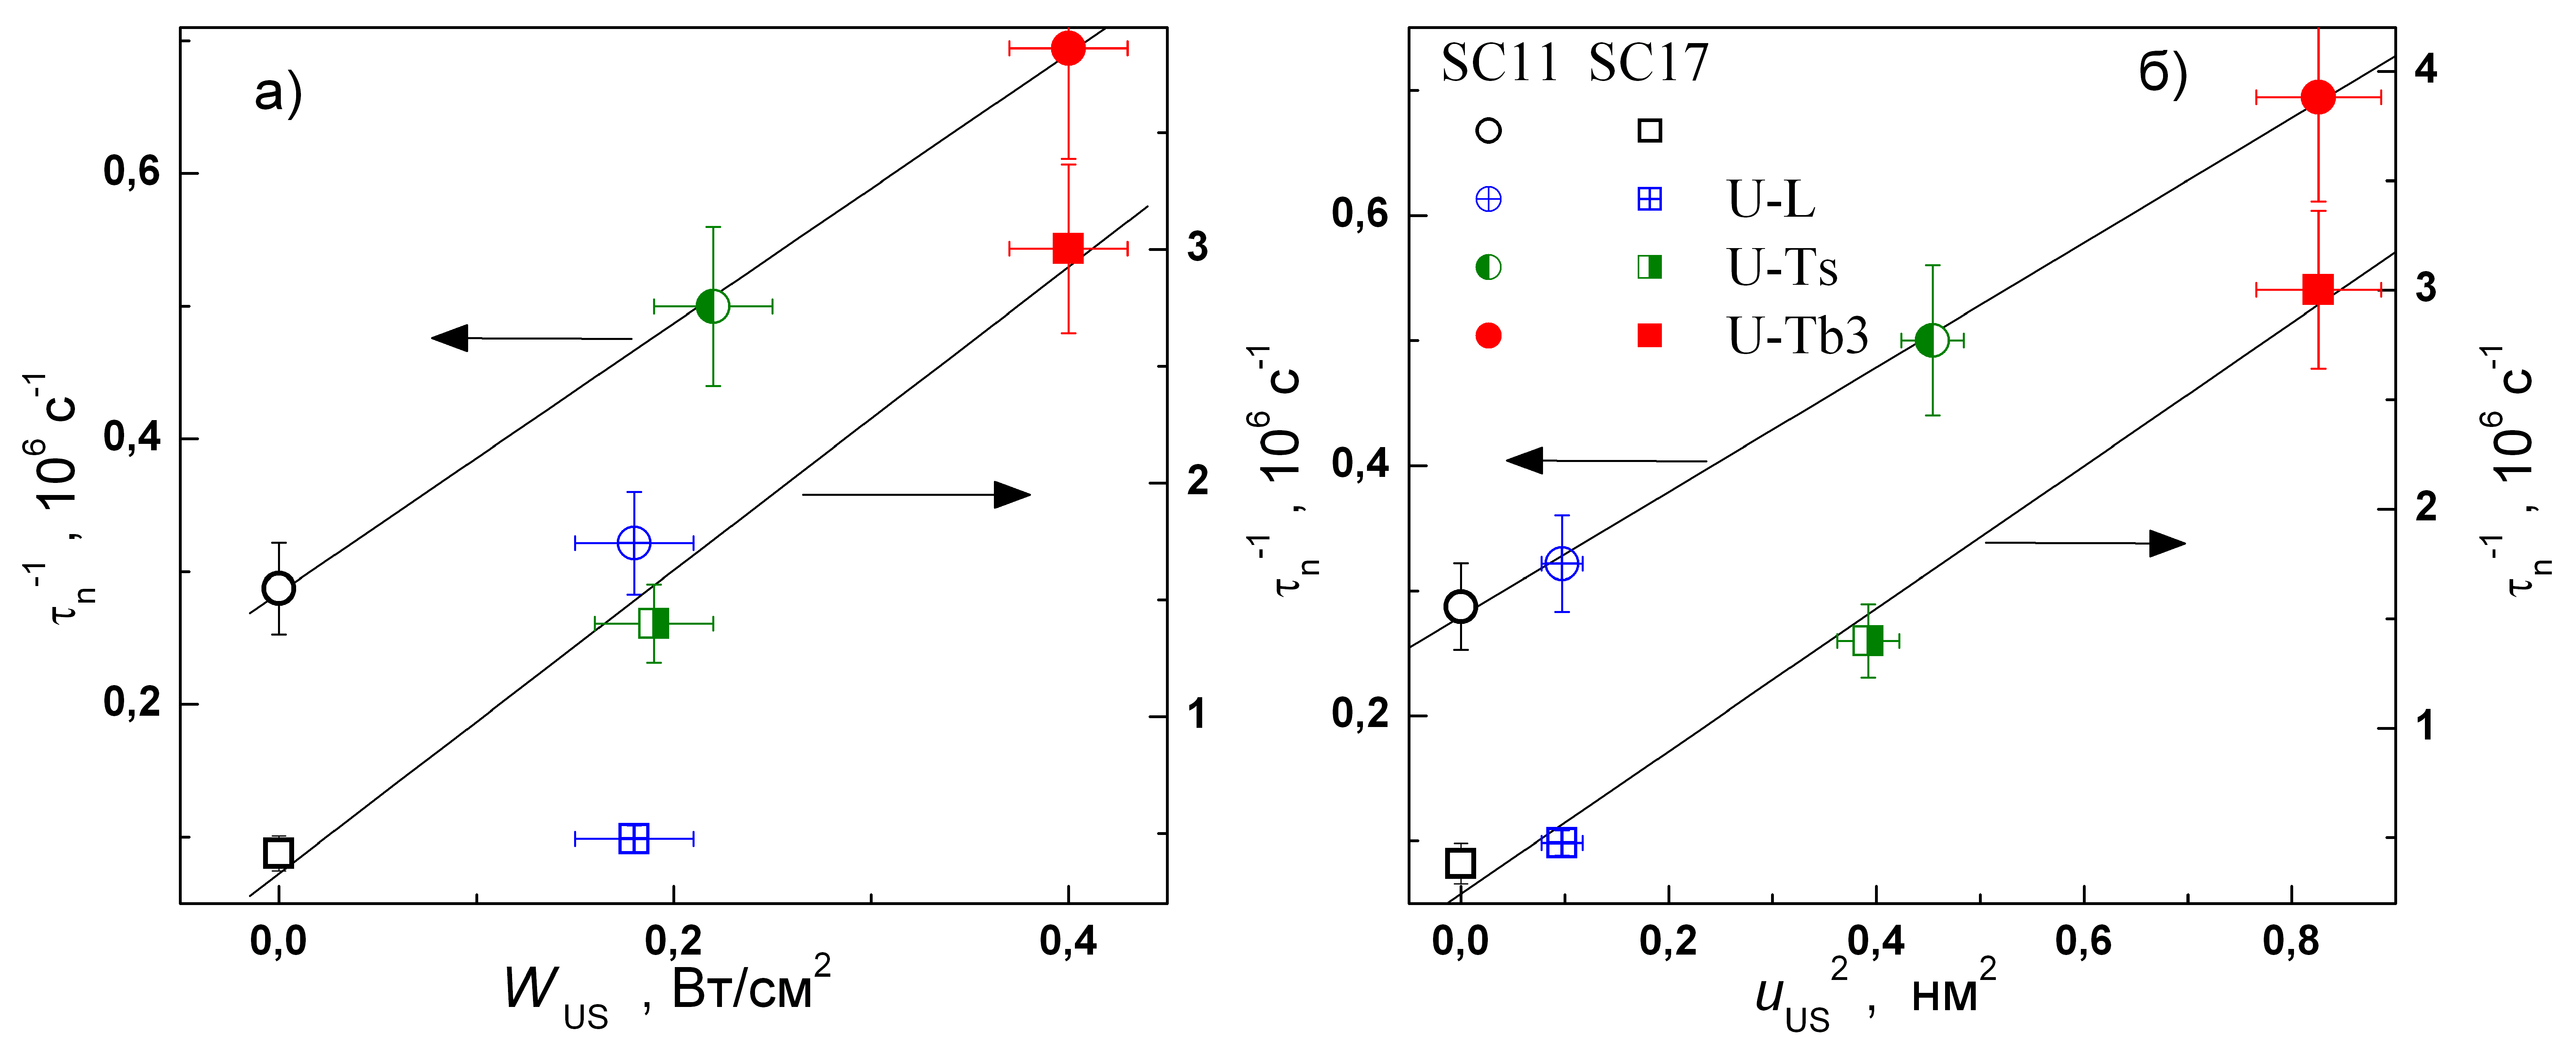
\includegraphics[width=1\textwidth]{figKus}%
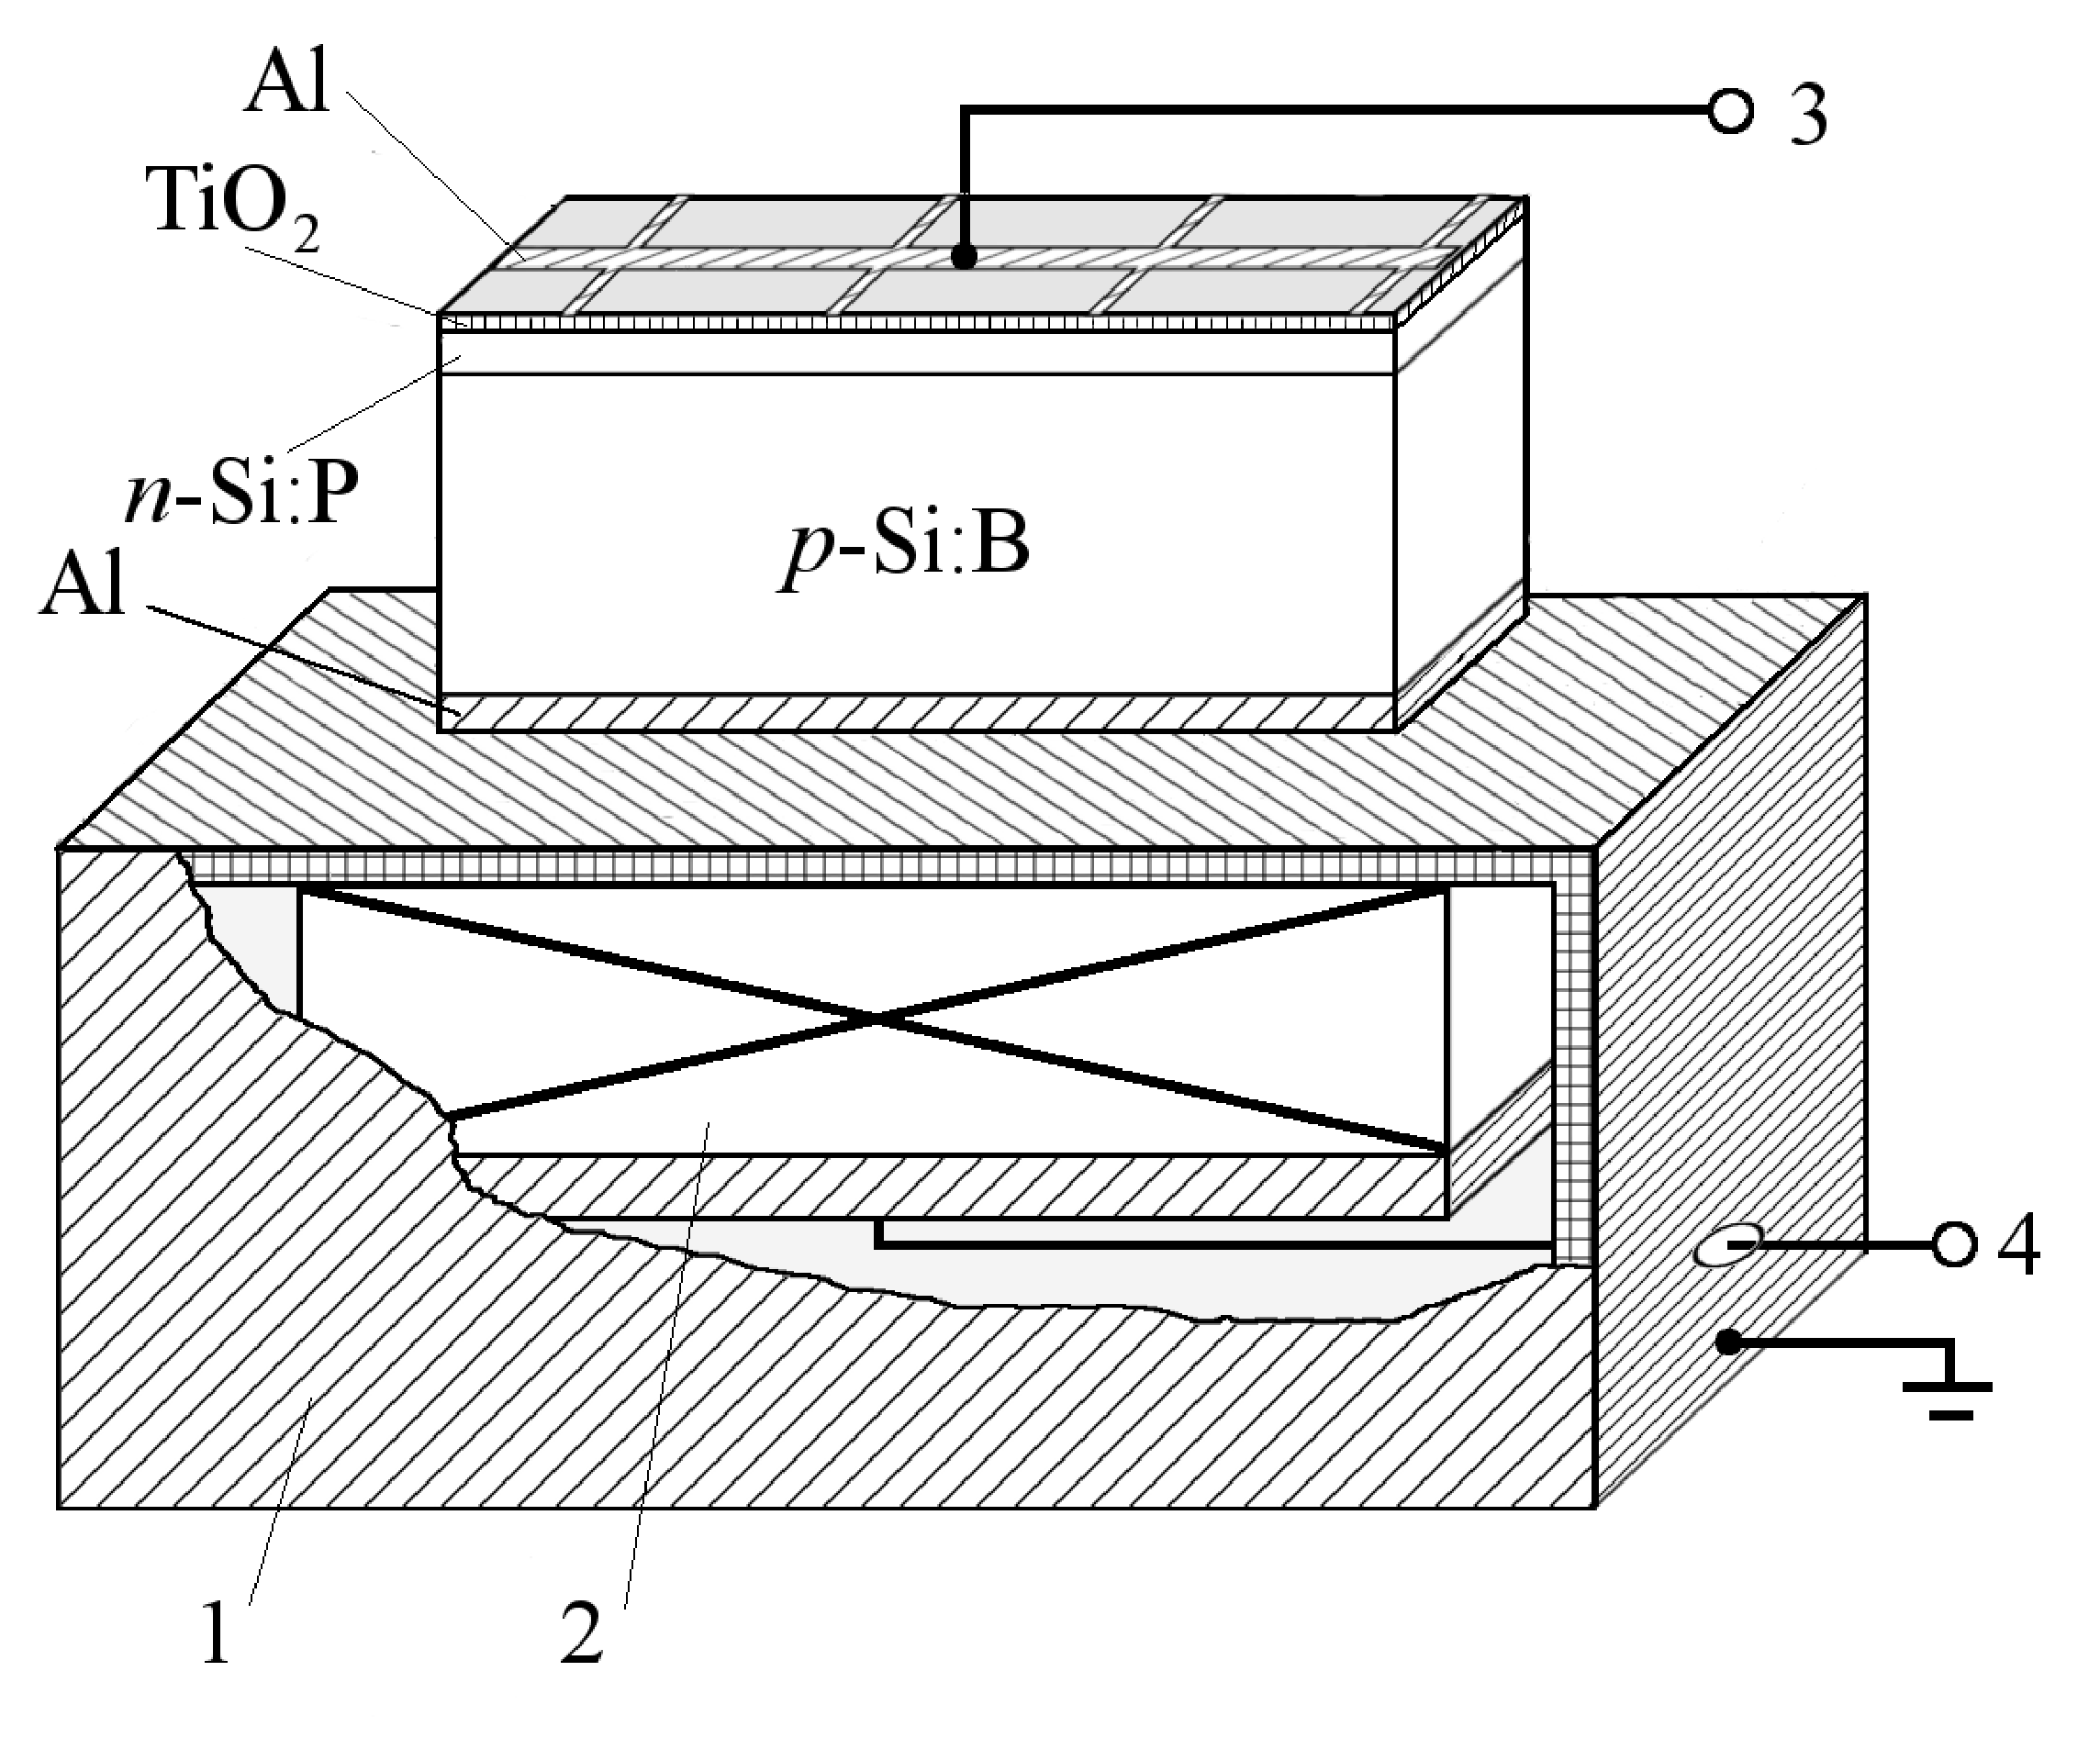
\includegraphics[width=0.4\textwidth]{USL_SC} \hfill
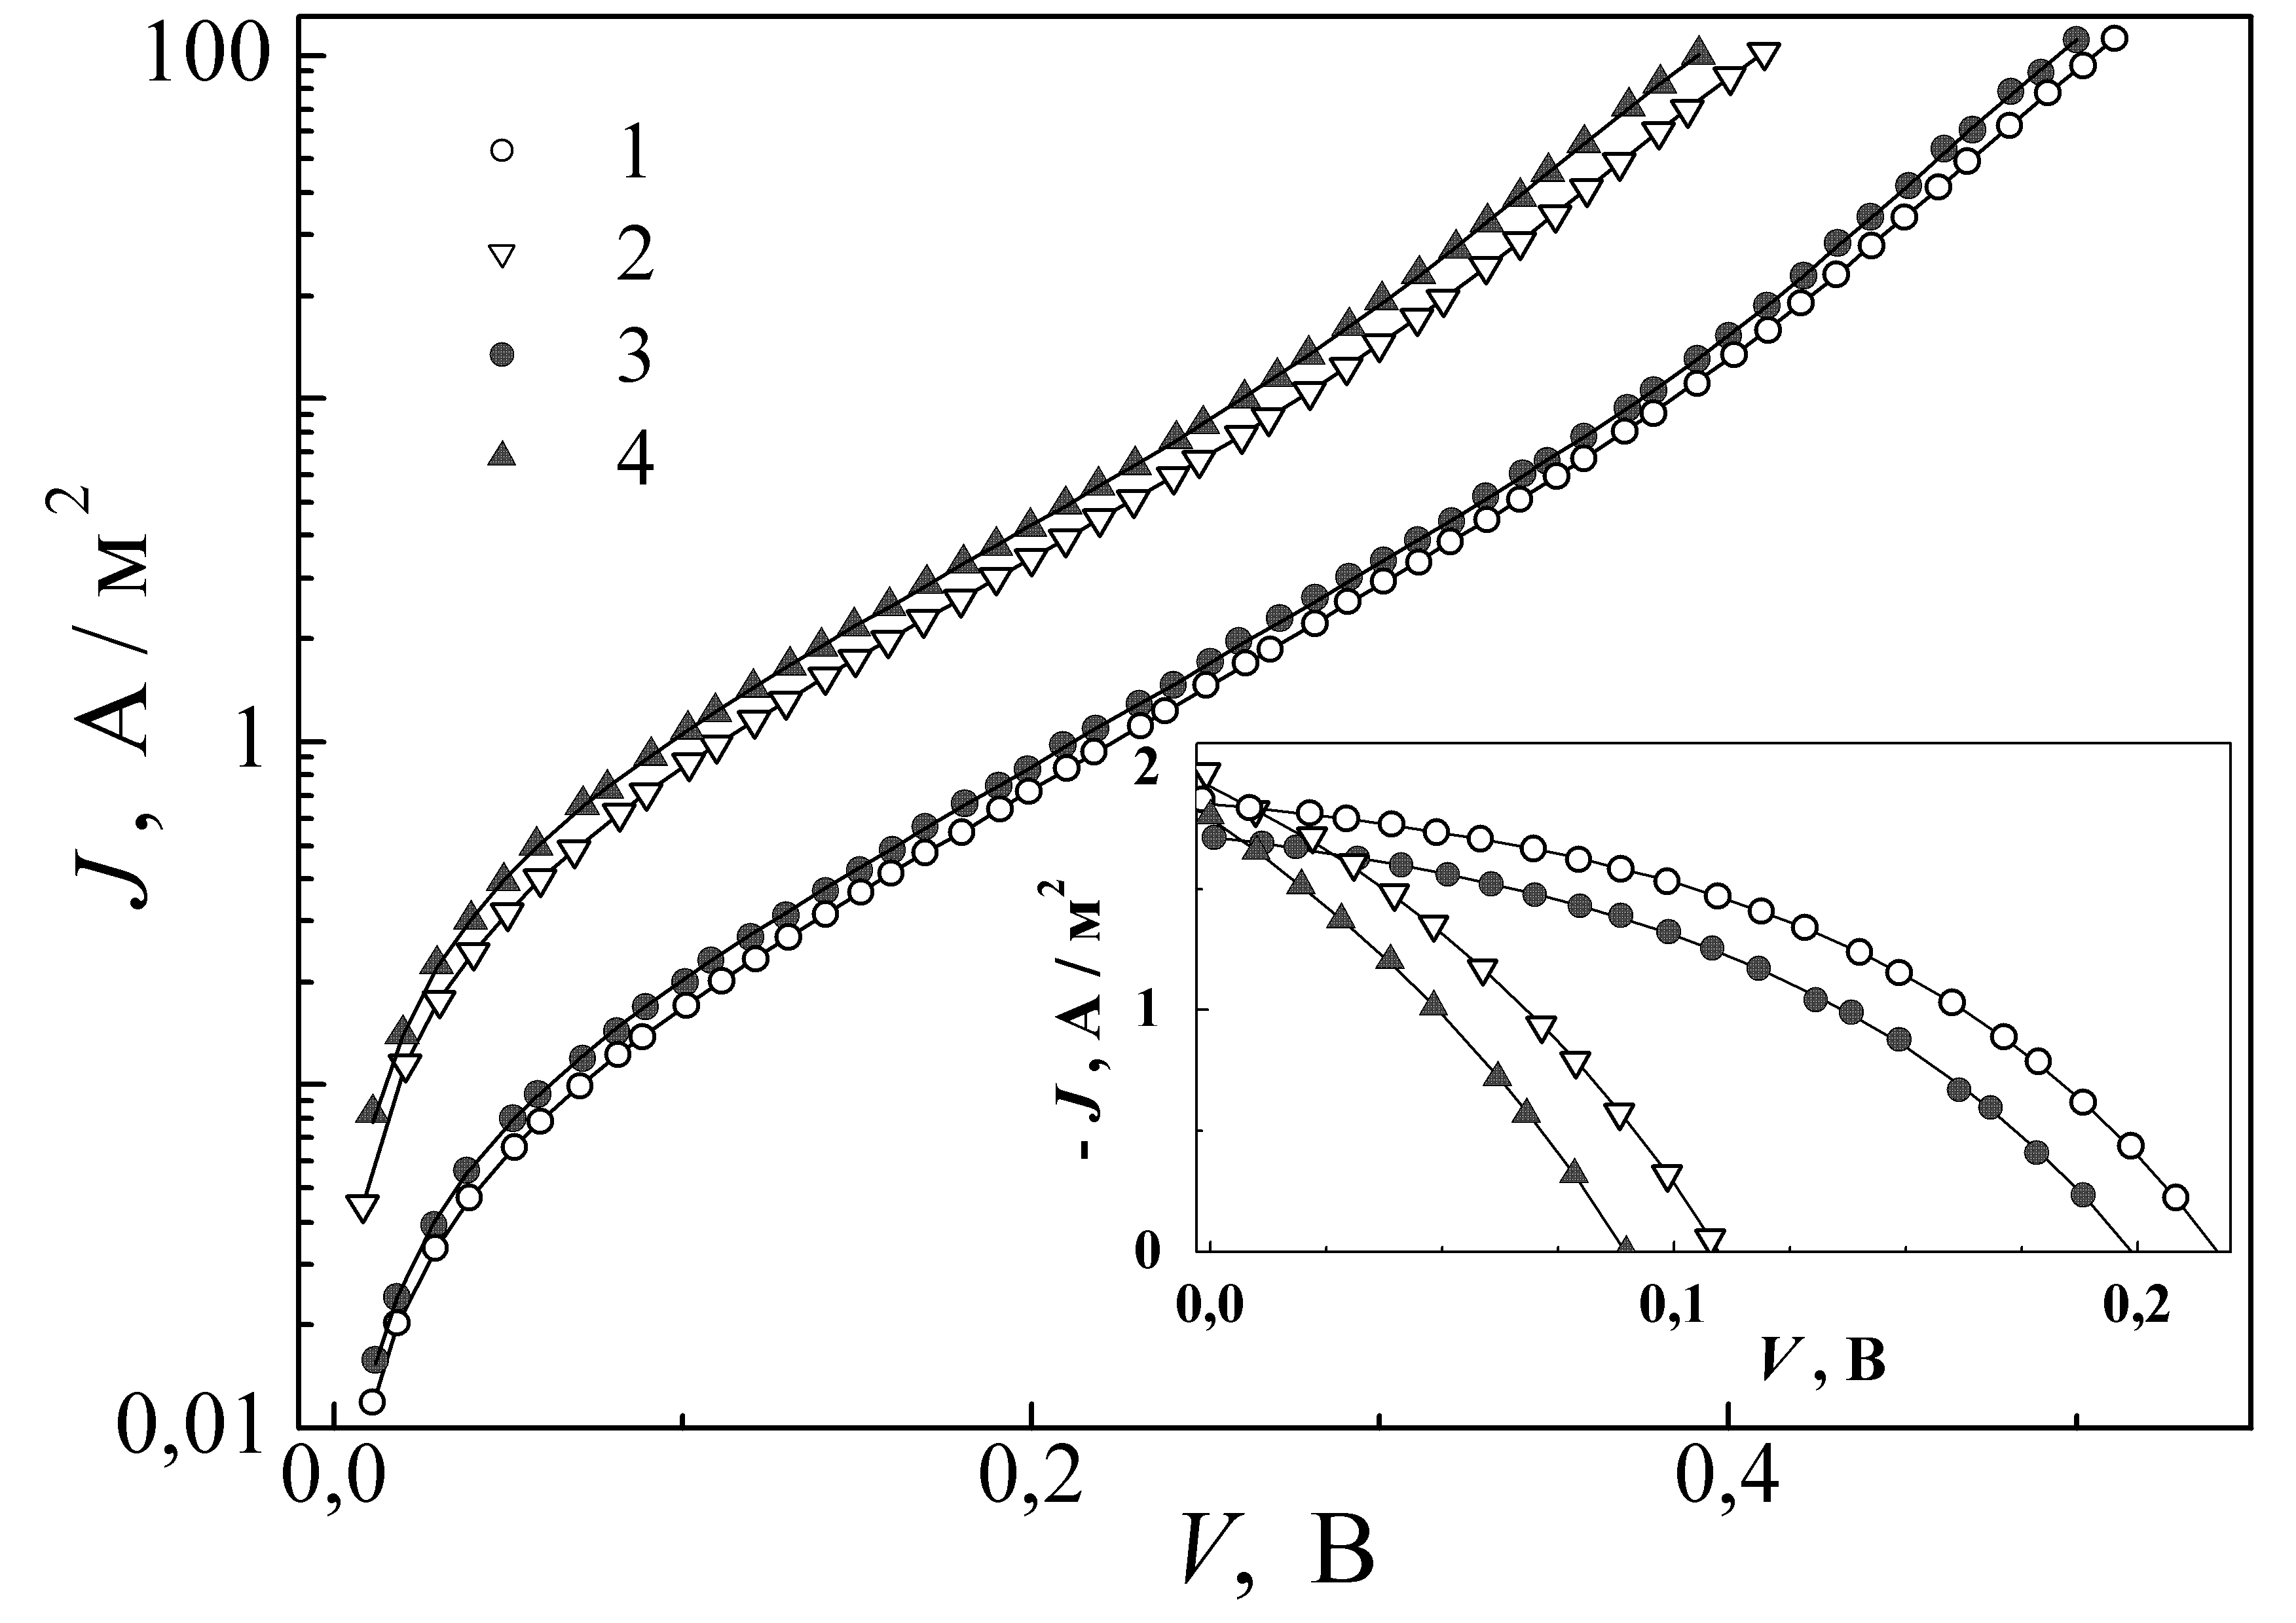
\includegraphics[width=0.5\textwidth]{figSSCIV}
\caption{\label{USL_SC}
Зліва --- схема УЗН.
1 --  екран;
2 --- п'єзоелектричний перетворювач;
3 --- контакти для вимірювання ВАХ;
4 --- контакти для збудження ультразвуку.
Справа --- типові ВАХ, виміряні при температурах 301~K (криві 1 та 2) та 341~K (2 та 4)
за умов УЗН (2, 4) та для акустично ненавантаженого зразка (1 та 3)
Точки --- експеримент, лінії --- апроксимація згідно з (\ref{eqSSCIV})
}%
\end{figure}

 Дослідження показали, що
   в діапазоні $290\div340$~К при УЗН (частота ультразвуку $f_\mathtt{US}=4\div8$~МГц, інтенсивність $W_\mathtt{US}\leq0,4$~Вт/см$^2$) у вихідних кремнієвих сонячних елементах  відбувається деградація
фотоелектричних властивостей, а саме
спостерігається зменшення густини струму короткого замикання $J_{sc}$ (до 10\%), напруги холостого ходу $V_{oc}$ (до 15\%) та фактору форми вольт--амперних характеристик (ВАХ) $F\!F$ (до 5\%).
Зміни оборотні, значення параметрів  після припинення УЗН  та витримки зразків при кімнатній температурі протягом декількох десятків хвилин повертаються до своїх вихідних значень.
Величини акустоіндукованих змін слабко залежать від температури, водночас при використанні поперечних хвиль зменшення параметрів більш суттєві, ніж у випадку повздовжніх хвиль з тією ж інтенсивністю.
Останнє свідчить про те, що ефективність впливу УЗ визначається насамперед зміщеннями атомів.

З метою встановлення фізичного механізму виявлених ефектів проведено дослідження впливу УЗН на такі електрофізичні параметри як
ефективний час життя носіїв заряду в області просторового заряду $\tau_{g}$,
фактор неідеальності $n_\mathrm{id}$,
час життя неосновних носіїв у базі діода $\tau_n$
та шунтуючий опір $R_{sh}$.
Визначення параметрів проводилось шляхом апроксимації ВАХ згідно з моделлю подвійного діода:
\begin{eqnarray}
\label{eqSSCIV}
\nonumber J(V,\,T)&=&-J_{ph}+\frac{qn_id}{2\tau_{g}}\left\{\exp \left[\frac{q(V-JR_s)}{n_\mathrm{id}kT}\right]-1\right\}+\\
&&+\frac{qn_i^2}{p_p}\sqrt{\frac{\mu_nkT}{\tau_n}}\left\{\exp \left[\frac{q(V-JR_s)}{kT}\right]-1\right\}+\frac{V-JR_s}{R_{sh}}\,,
\end{eqnarray}
де
$J$ --- густина струму,
$V$ --- прикладена напруга,
$J_{ph}$ --- густина фотогенерованого струму,
$n_i$ --- концентрація власних носіїв заряду,
$d$ --- товщина області просторового заряду,
$p_p$ --- концентрація основних носіїв заряду в $p$--області,
%$E_g$ --- ширина забороненої зони напівпровідника,
%$N_c$ та $N_v$ --- ефективна густина станів поблизу дна зони провідності та вершини валентної зони, відповідно;
%$n_\mathrm{id}$ --- фактор неідеальності
$R_s$ --- послідовний опір,
$\mu_n$ --- рухливість неосновних носіїв у базі діода.
При апроксимації (рис.~\ref{USL_SC}) використовувався метод диференційної еволюції та враховувались температурні та польові залежності $n_i$, $d$, $\mu_n$.
 %величини  $\tau_g$, $\tau_n$, $n_{\mathrm{id}}$, $R_{sh}$, $R_s$ та  $J_{ph}$ розглядалися як невідомі (шукані).
Крім того, оцінка $\tau_n$ проводилася за температурною залежністю струму короткого замикання.

Виявлені температурні залежності величин $n_\mathrm{id}$ та $\tau_g$
($n_{\mathrm{id}}(T) \sim T_{\mathrm{id}}/T$,
$\tau_{g}(T)\sim\exp\left(-E_{\tau g}/kT\right)$,
де $T_{\mathrm{id}}$ та $E_{\tau g}$ певні характерні величини),
а також їх абсолютні значення ($n_{\mathrm{id}}>2$, $\tau_{g}\approx(10^{-8}\div10^{-7})$~c),
свідчать, що рекомбінація в області просторового заряду досліджених структур
відбувається відповідно до
моделі рекомбінації в системі спарених рівнів двох окремих дефектів
%(CDLR, coupled defect level recombination)
%\cite{CDLR:JAP}
[1$^*$].
УЗН викликає оборотне зростання $n_\mathrm{id}$  (до 0,04) та зменшення $\tau_g$ (до 30\%).
Оборотність акустоіндукованих змін та незмінність $T_{\mathrm{id}}$ і $E_{\tau g}$
вказують на
сталість концентрації рекомбінаційних центрів та відсутність їх перебудова при УЗН.
Дослідження також показали, що
а)~рекомбінація у квазі--нейтральній області може бути описана в рамках моделі Шоклі--Ріда--Хола,
%(SRH), при цьому $\tau_n^{-1}=\sum_i N_{d,i}\,\,\sigma_{n,i}\,\upsilon_{\mathrm{th},n}$
%(де
%кількість доданків в сумі визначається загальним числом різних РЦ,
%кожний з яких характеризуються концентрацією $N_{d,i}$ та поперечним перерізом захоплення (ППЗ) електронів $\sigma_{n,i}$;
%$\upsilon_{\mathrm{th},n}$ --- теплова швидкість електронів).
б)~величина $\tau_n$, яка безпосередньо пов'язана з цими процесами,
при УЗН суттєво (до 90\%) зменшується,
причому
$\tau_{n}^{-1}\sim u_\mathtt{US}^2$ (де $u_\mathtt{US}$ --- амплітуда зміщень атомів при поширенні ультразвуку).

З метою визначення типів основних рекомбінаційних центрів
було проведено дослідження впливів інтенсивного ($2$~кВт/м$^2$) довготривалого (до  $15$~год) освітлення
та відпалу (при 200~$^\circ$C) на параметри сонячних елементів.
Аналіз залишкових змін та перехідних процесів після припинення освітлення засвідчив, що дефектами, які приймають участь як у рекомбінаційних процесах, так і у акусто--дефектнiй взаємодiї є кисневмiснi преципiтати (переважно) та
пари Fe$_i$B$_s$ (частково).
Цей висновок також підтверджено за допомогою методу диференційним коефіцієнтів ВАХ
%\cite{Bulyar}
[4$^*$],
застосування якого дозволило з'ясувати, що основними дефектами в області просторового заряду вихідних сонячних елементів є кисневмiснi преципiтати  (яким відповідають рівні у забороненій зоні з розташуванням  $E_c-(0,46\div0,48)$~еВ та $E_c-0,40$~еВ), дислокації ($E_c-0,36$~еВ) та комплекси Fe$_i$O$_i$ ($E_c-0,43$~еВ).
Додатково показано, що
при УЗН відбувається незначне (близько 10~меВ) зменшення енергії активації та збільшується внесок
у рекомбінацію більш мілких рівнів, зокрема пов'язаних з преципiтатами, причому зміни відносних внесків різних центрів лінійно залежать від $u_\mathtt{US}$.

Виявлено оборотне зменшення величини шунтуючого опору (до 30\%) при УЗН.
Спираючись на температурну залежність $R_{sh}$ показано, що його поява може бути описана в рамках моделі дислокаційно--індукованого імпедансу
%\cite{Rsh:Gopal2004}
[2$^*$], а акустоіндуковані зміни викликані зростанням ефективності захоплення електронів лінійними дефектами, розташованими в області $p$--$n$ переходу.

Проведені в рамках дводіодної моделі числові розрахунки показали, що акустоіндуковані зміни $J_{sc}$ пов'язані зі зменшенням $\tau_{n}$,
тоді як зменшення $\tau_{g}$ викликає деградацію як $V_{oc}$, так i $F\!F$.
Ефект деградації підсилюється внаслідок акустоіндукованого зменшення $R_{sh}$ та частково компенсується зростанням $n_\mathrm{id}$.

Для пояснення виявлених ефектів запропонована модель акустоактивного комплексного рекомбінаційного центру, який складається з нееквівалентних компонент.
При поширенні акустичної хвилі на точковий дефект дії періодична сила, амплітуда якої залежить від зміни об'єму кристалу, що припадає на один дефект $\Delta\Omega_d$
%\cite{MirzadeJAP2011}
[3$^*$] ($\Delta\Omega_d<0$ для дефектів вакансійного типу).
В рамках запропонованої моделі за умов УЗН компоненти (якими у випадку рекомбінації в системі спарених рівнів є  дефекти донорного та акцепторного типу, а при рекомбінації Шоклі--Ріда--Хола --- частини комплексного точкового рекомбінаційного центру) здійснюють гармонічні коливання, частота та вісь яких
визначаються акустичною хвилею, тоді як амплітуди та фази залежить також і від  $\Delta\Omega_d^\mathtt{D}$ та
$\Delta\Omega_d^\mathtt{A}$ кожної з них --- рис.~\ref{fig_Model}.
При цьому відстань між компонентами при УЗН $r_\mathtt{US}$ залежить від часу

\begin{figure}[b]
\center
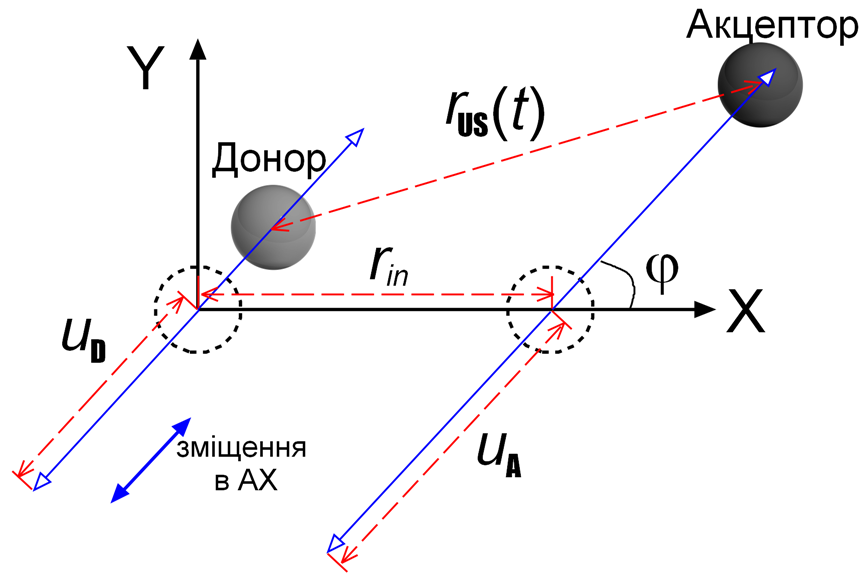
\includegraphics[width=0.5\textwidth]{fig_Model}
\caption{\label{fig_Model}
Модель поведінки дефектного комплексу за умов УЗН
}%
\end{figure}


\begin{multline}
\label{eqrUS}
r_\mathtt{US}(t)=\left\{[r_{in}+u_\mathtt{A}\cos(2\pi f_\mathtt{US}t+\delta)-u_\mathtt{D}\cos(2\pi f_\mathtt{US}t)]^2\cos^2\varphi \right.\\
    \left.+ [u_\mathtt{A}\cos(2\pi f_\mathtt{US}t+\delta)-u_\mathtt{D}\cos(2\pi f_\mathtt{US}t)]^2\sin^2\varphi\right\}^{0.5}\,,
\end{multline}
де
$r_{in}$ --- вихідна відстань,
$u_\mathtt{D}$ та $u_\mathtt{A}$ --- амплітуди коливань компонент, $u_\mathtt{D},\,u_\mathtt{A}\sim u_\mathtt{US}$,
%$\omega_\mathtt{US}$ --- циклічна частота УЗ,
$\delta$ --- зсув фаз між коливаннями компонент,
$\varphi$ --- кут між віссю комплексу та напрямом зміщень в акустичній хвилі.
В рамках запропонованої моделі проведено розрахунки очікуваних акустоіндукованих змін поперечного перерізу захоплення $\sigma_{n}$ та параметра зв'язку,
які визначають темп зникнення нерівноважних носіїв
у вищеназваних рекомбінаційних моделях.
Зокрема
а)~розглянуто ефективність впливу УЗН при збудженні поперечних та повздовжніх хвиль із врахуванням наявності просторово орієнтованих дислокацій та показано, що найбільші зміни очікуються у випадку, коли комплекс складається з компонент міжвузольного та вакансійного типу $(\Delta\Omega_d^\mathtt{D}\cdot\Delta\Omega_d^\mathtt{A}<0)$
 в умовах поперечних коливань;
б)~показано, що збільшення $\sigma_{n}$ та зменшення параметра зв'язку має викликати зменшення $\tau_g$ та зростання $n_\mathrm{id}$, що спостерігається на експерименті;
в)~при УЗН має бути справедливим співвідношення
\begin{equation}
\label{eqEpsSigUSA}
\tau_{n,\mathtt{US}}^{-1}=
\tau_{n,in}^{-1}+u_{\mathtt{US}}^2\,\sum_j\,N_{d,j}\,\sigma_{n,j}^{in}\,K_\mathtt{US,j}\,\upsilon_{\mathrm{th},n}\,,
\end{equation}
де
кількість доданків у сумі визначається загальним числом різних акустоактивних рекомбінаційних центрів,
кожний з яких характеризуються концентрацією $N_{d,j}$,
$\upsilon_{\mathrm{th},n}$ --- теплова швидкість електронів
$K_\mathtt{US,j}$ описує взаємодію ультразвуку з дефектом $j$--го типу.

%(SRH), при цьому $\tau_n^{-1}=\sum_i N_{d,i}\,\,\sigma_{n,i}\,\upsilon_{\mathrm{th},n}$
%(де
%кількість доданків в сумі визначається загальним числом різних РЦ,
%кожний з яких характеризуються концентрацією $N_{d,i}$ та поперечним перерізом захоплення (ППЗ) електронів $\sigma_{n,i}$;
%$\upsilon_{\mathrm{th},n}$ --- теплова швидкість електронів).



В розділі також представлені результати досліджень впливу УЗН на властивості кремнієвих сонячних елементів,
опромінених $\gamma$--квантами $^{60}$Co (дози $10^6$ і $10^7$~рад) та реакторними нейтронами (флюєнс $4\cdot10^{11}$~см$^{-2}$).
Використовуючи літературні дані показано, що при нейтронному опроміненні виникають пари C$_i$O$_i$,
вакансійні кластери V$_n$ та пари VO$_i$, тоді як $\gamma$--промені викликають появу лише C$_i$O$_i$ та VO$_i$;
проведено оцінку концентрацій радіаційних дефектів та їх впливу на $\tau_n$.

\begin{figure}[ht]
\center
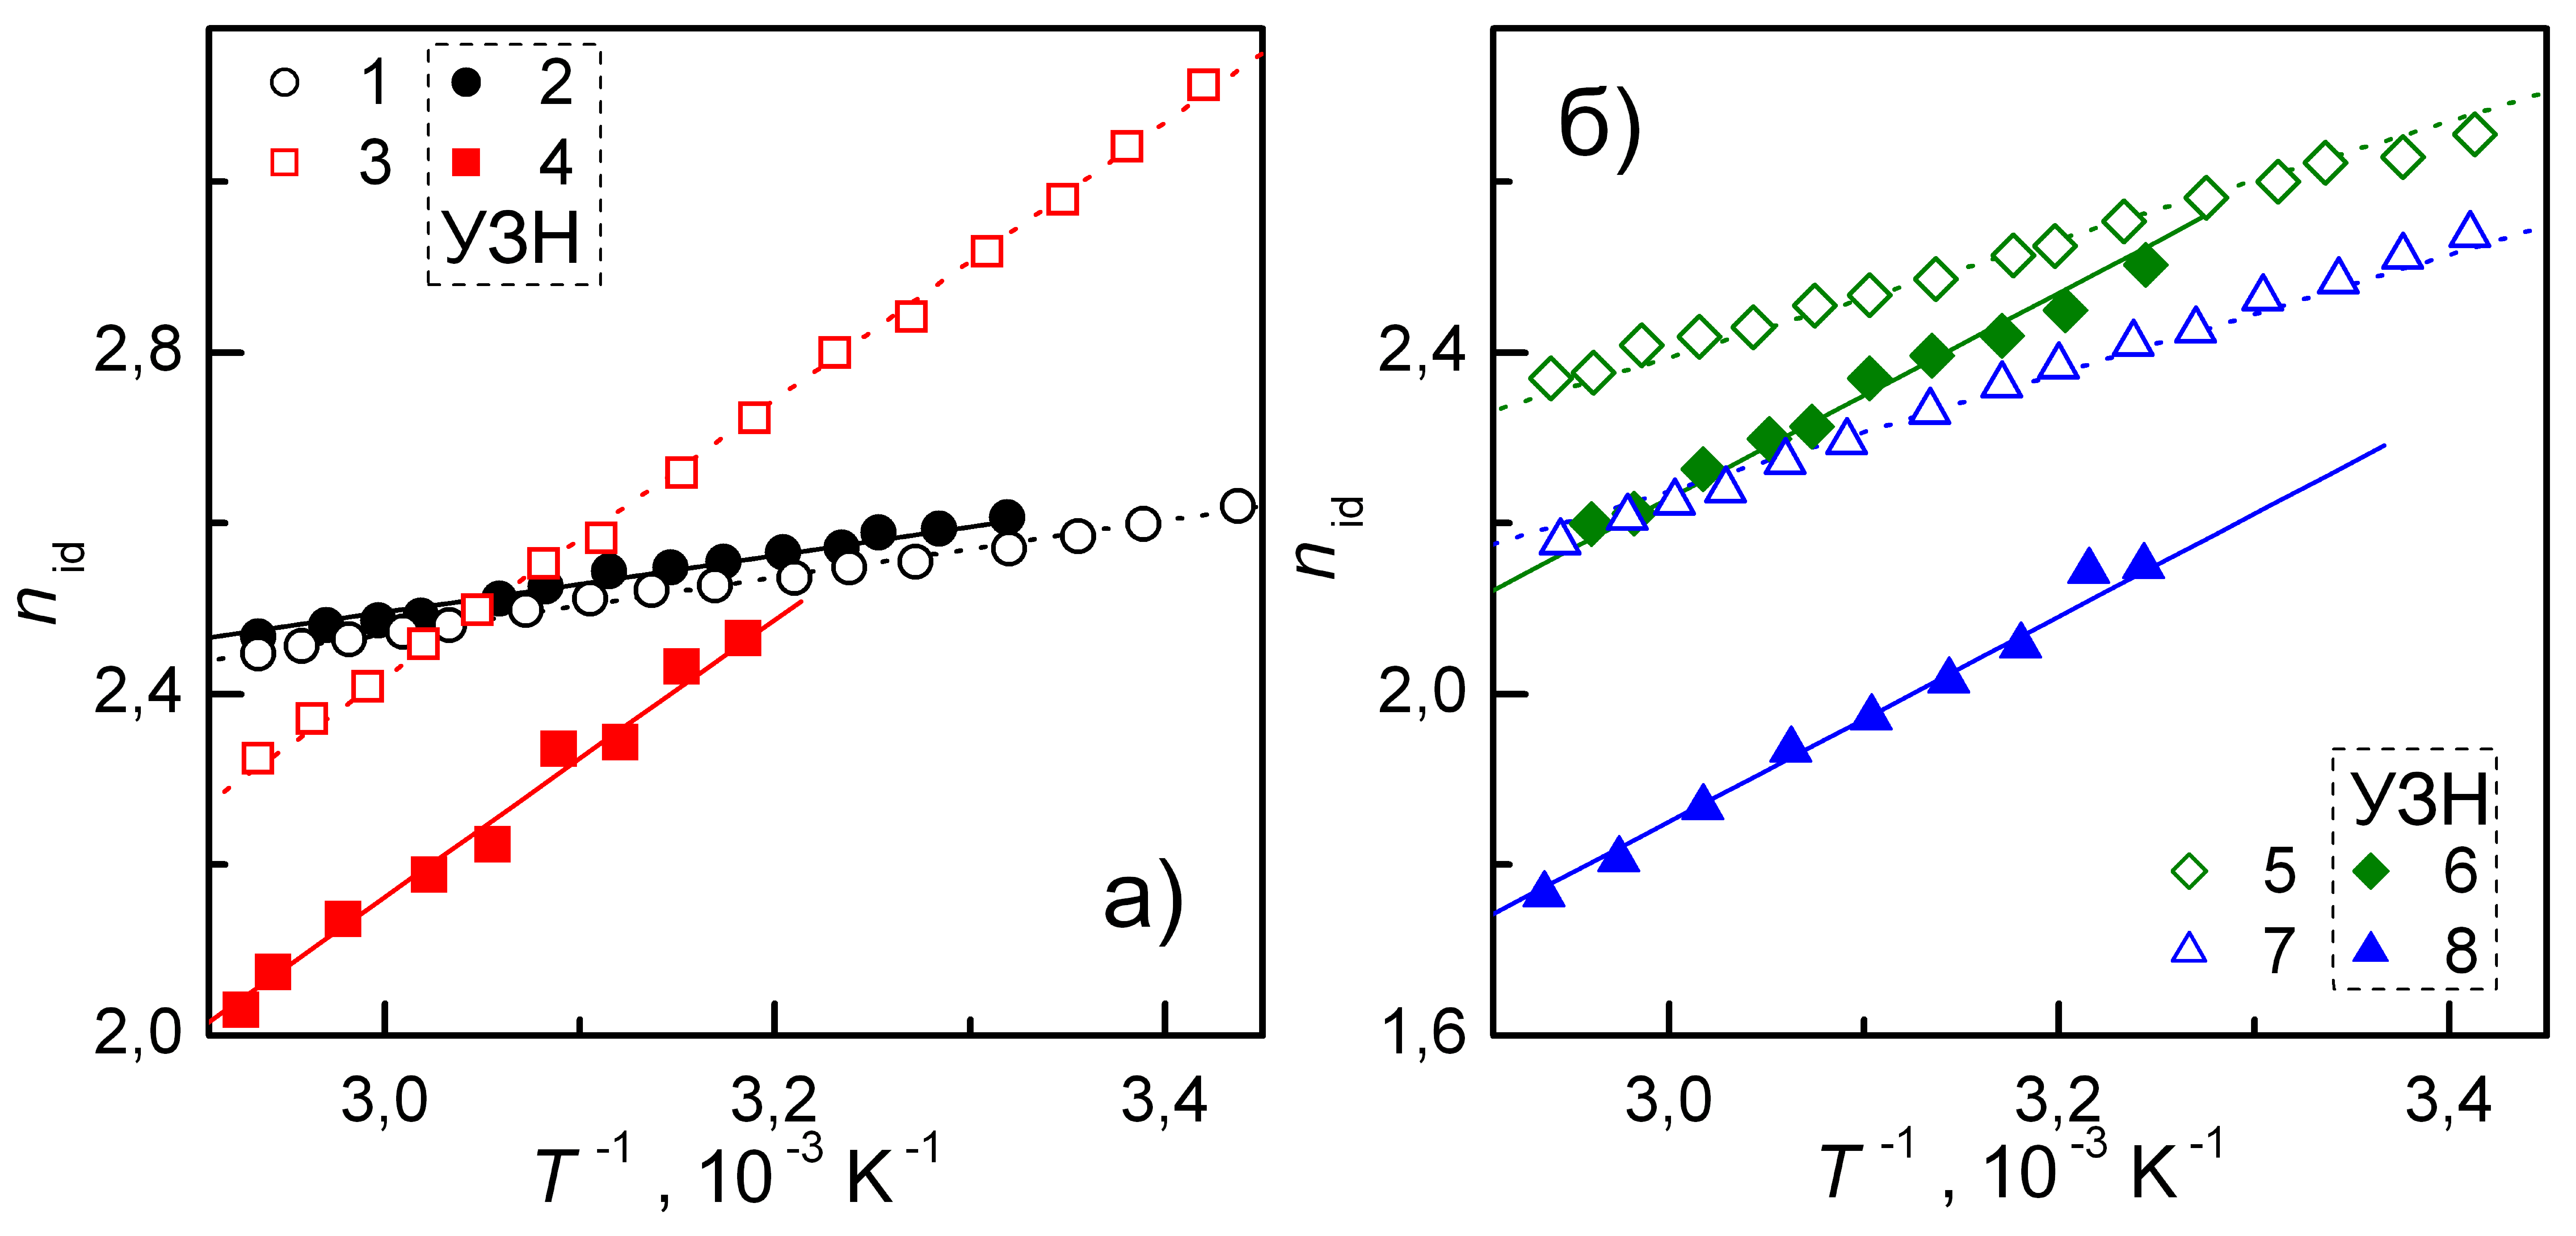
\includegraphics[width=0.9\textwidth]{fignRD}%
\caption{\label{fignRD}
Температурні залежності фактора неідеальності
для неопроміненого (криві 1, 2),
нейтронно--опроміненого (3, 4) та
$\gamma$--опромінених (5, 6 та 7, 8 для доз $10^6$ та $10^7$~рад, відповідно)
зразків.
Криві 1, 3, 5 та 6 отримані без УЗН,
криві 2, 4, 9 та 8 відповідають УЗН (поперечні хвилі; 4,2~МГц; 0,4~Вт/см$^2$)
}%
\end{figure}


\begin{figure}[t]
\center
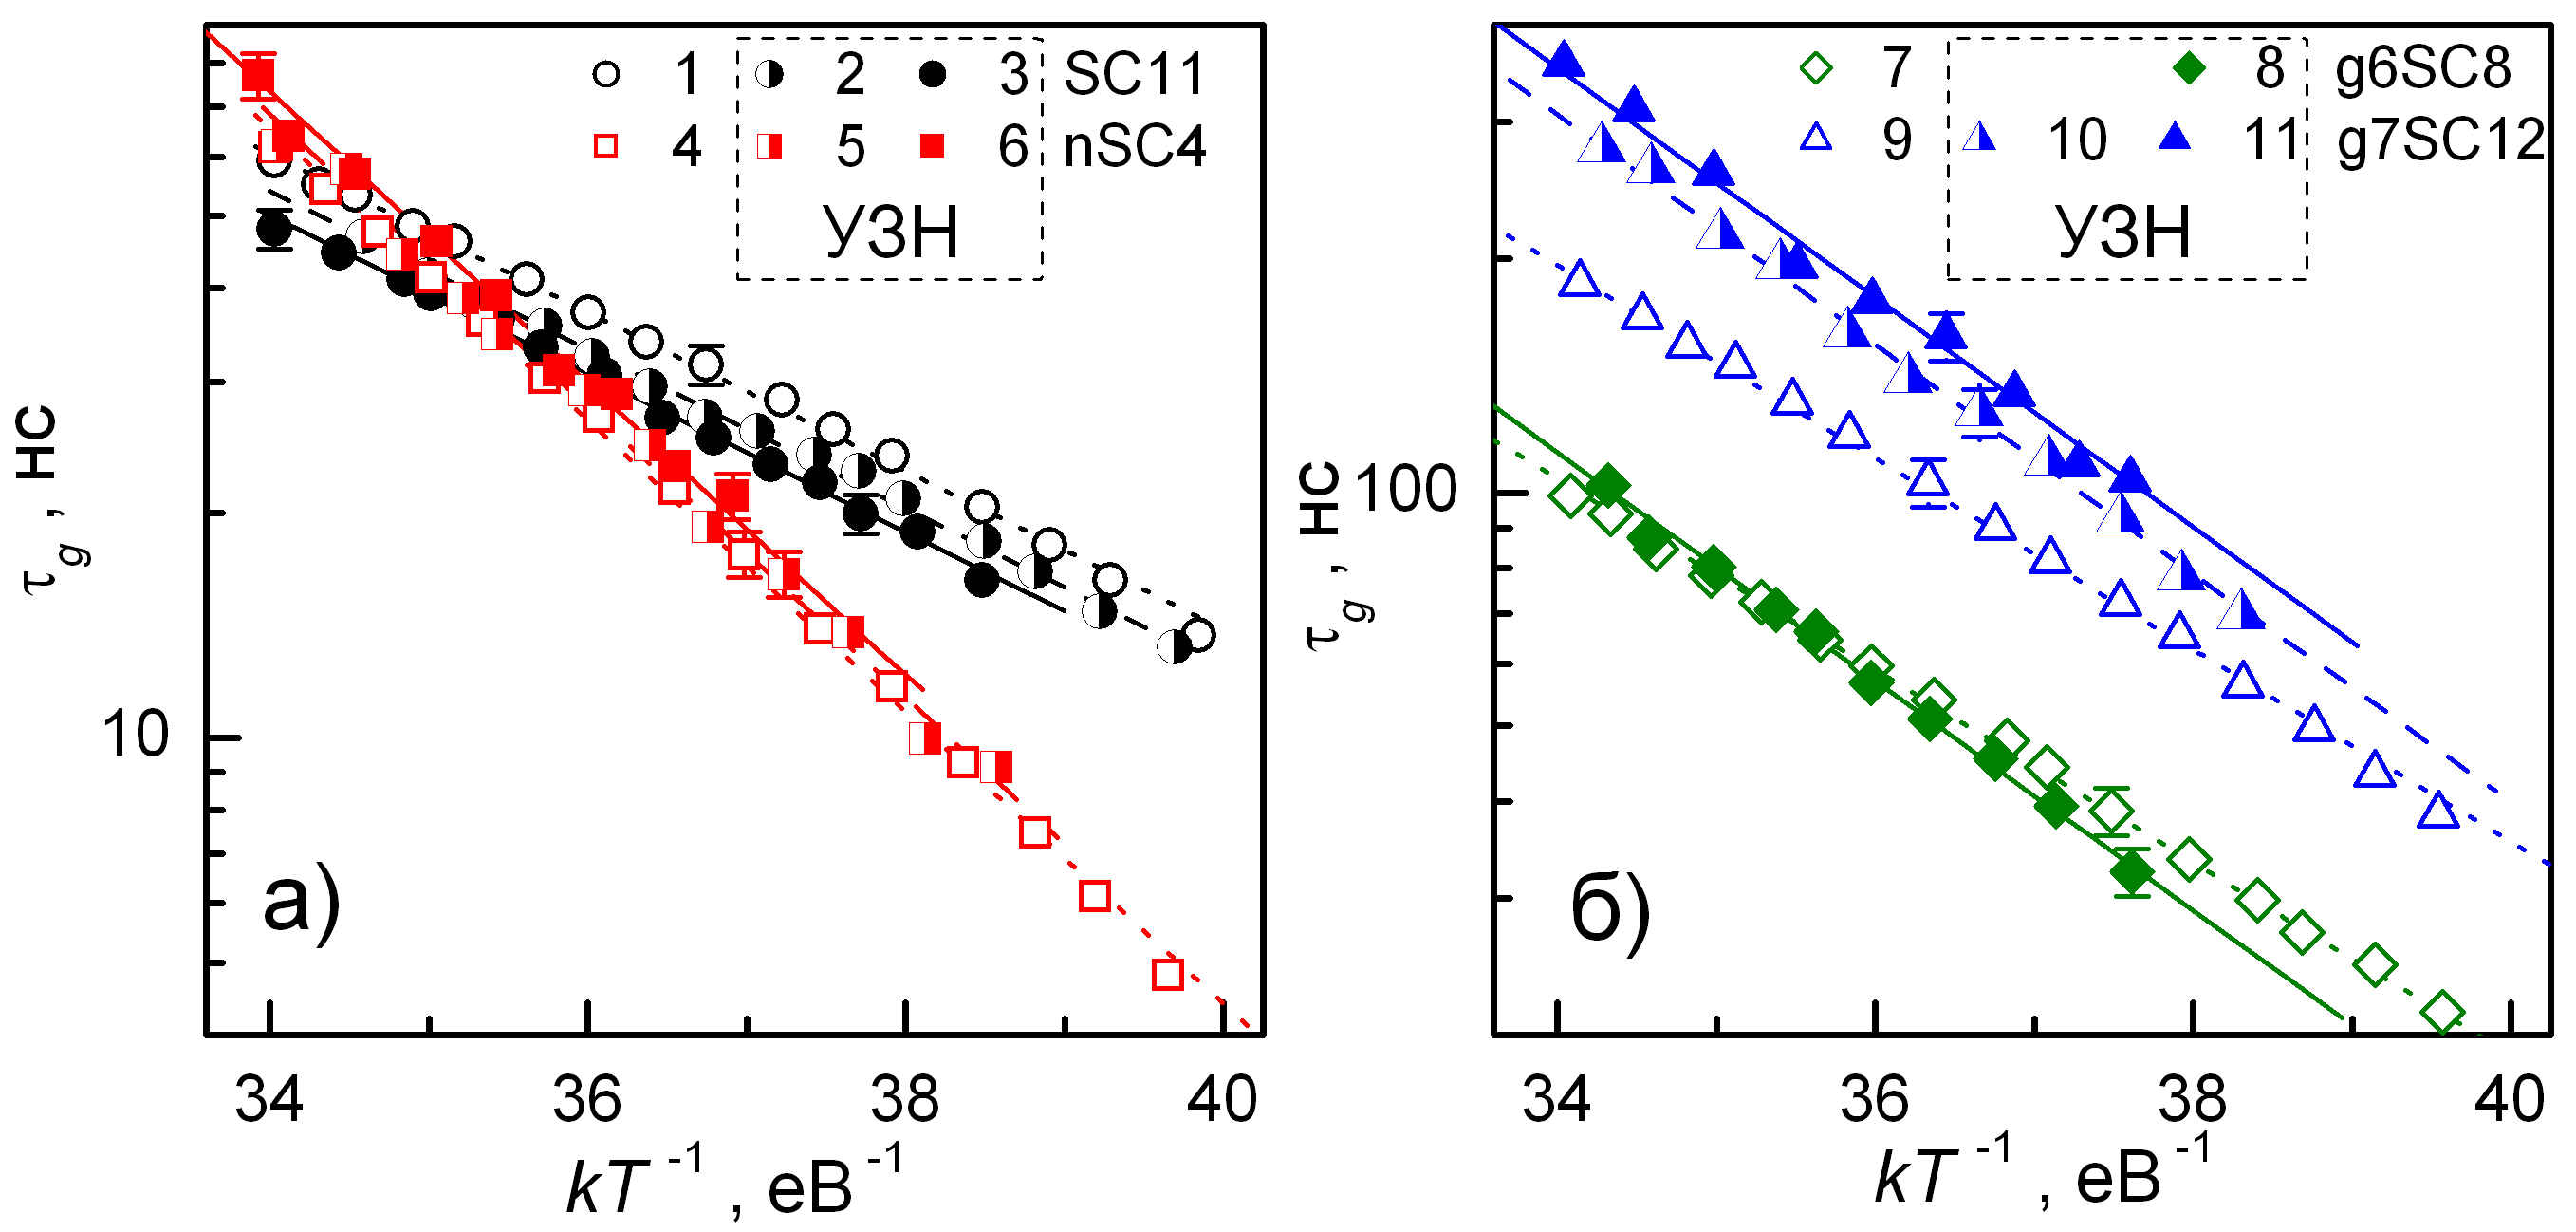
\includegraphics[width=0.9\textwidth]{figTAUgRD}%
\caption{\label{figTAUgRD}
Температурні залежності $\tau_g$.
Позначення кривих збігаються з рис.~\ref{fignRD}
}%
\end{figure}

Проведені дослідження показали, що
а)~характер температурних залежностей  $\tau_{g}$ та $n_\mathrm{id}$ співпадає з вихідними структурами (рис.~\ref{fignRD} та \ref{figTAUgRD}), проте зміна $T_{\mathrm{id}}$ та $E_{\tau g}$ вказує на участь радіаційних дефектів в процесах рекомбінації в системі спарених рівнів;
б)~акустоіндуковані зміни $n_\mathrm{id}$ в радіаційно модифікованих структурах більші за величиною та протилежні за знаком до змін у вихідних сонячних елементах;
в рамках моделі акустоактивного комплексного рекомбінаційного центру це свідчить про те, що до опромінення $\Delta\Omega_d^\mathtt{D}\cdot\Delta\Omega_d^\mathtt{A}>0$, а після $\Delta\Omega_d^\mathtt{D}\cdot\Delta\Omega_d^\mathtt{A}<0$;
в)~за умов УЗН величини $T_{\mathrm{id}}$ та $E_{\tau g}$ у $\gamma$--опромінених структурах оборотно змінюються,
що засвідчує акустоіндуковану перебудову метастабільного дефекту (VO$_i$).
Виявлено, що при УЗН величина $\tau_n^{-1}$ для опромінених структур також лінійно залежить від $u_{\mathtt{US}}^2$.
Використовуючи співвідношення~(\ref{eqEpsSigUSA}), визначено коефіцієнти, які характеризують взаємодію акустичних хвиль з радіаційними дефектами (для C$_i$O$_i$ $K_\mathtt{US}^\mathtt{CO}=0$, тобто цей дефект не є акустоактивним,
для дивакансії $K_\mathtt{US}=(42\pm15)$~см$^2$~Вт$^{-1}$)
та кисневмiсними преципiтатами ($K_\mathtt{US}>5$~см$^2$~Вт$^{-1}$).

\begin{figure}[ht]
\center
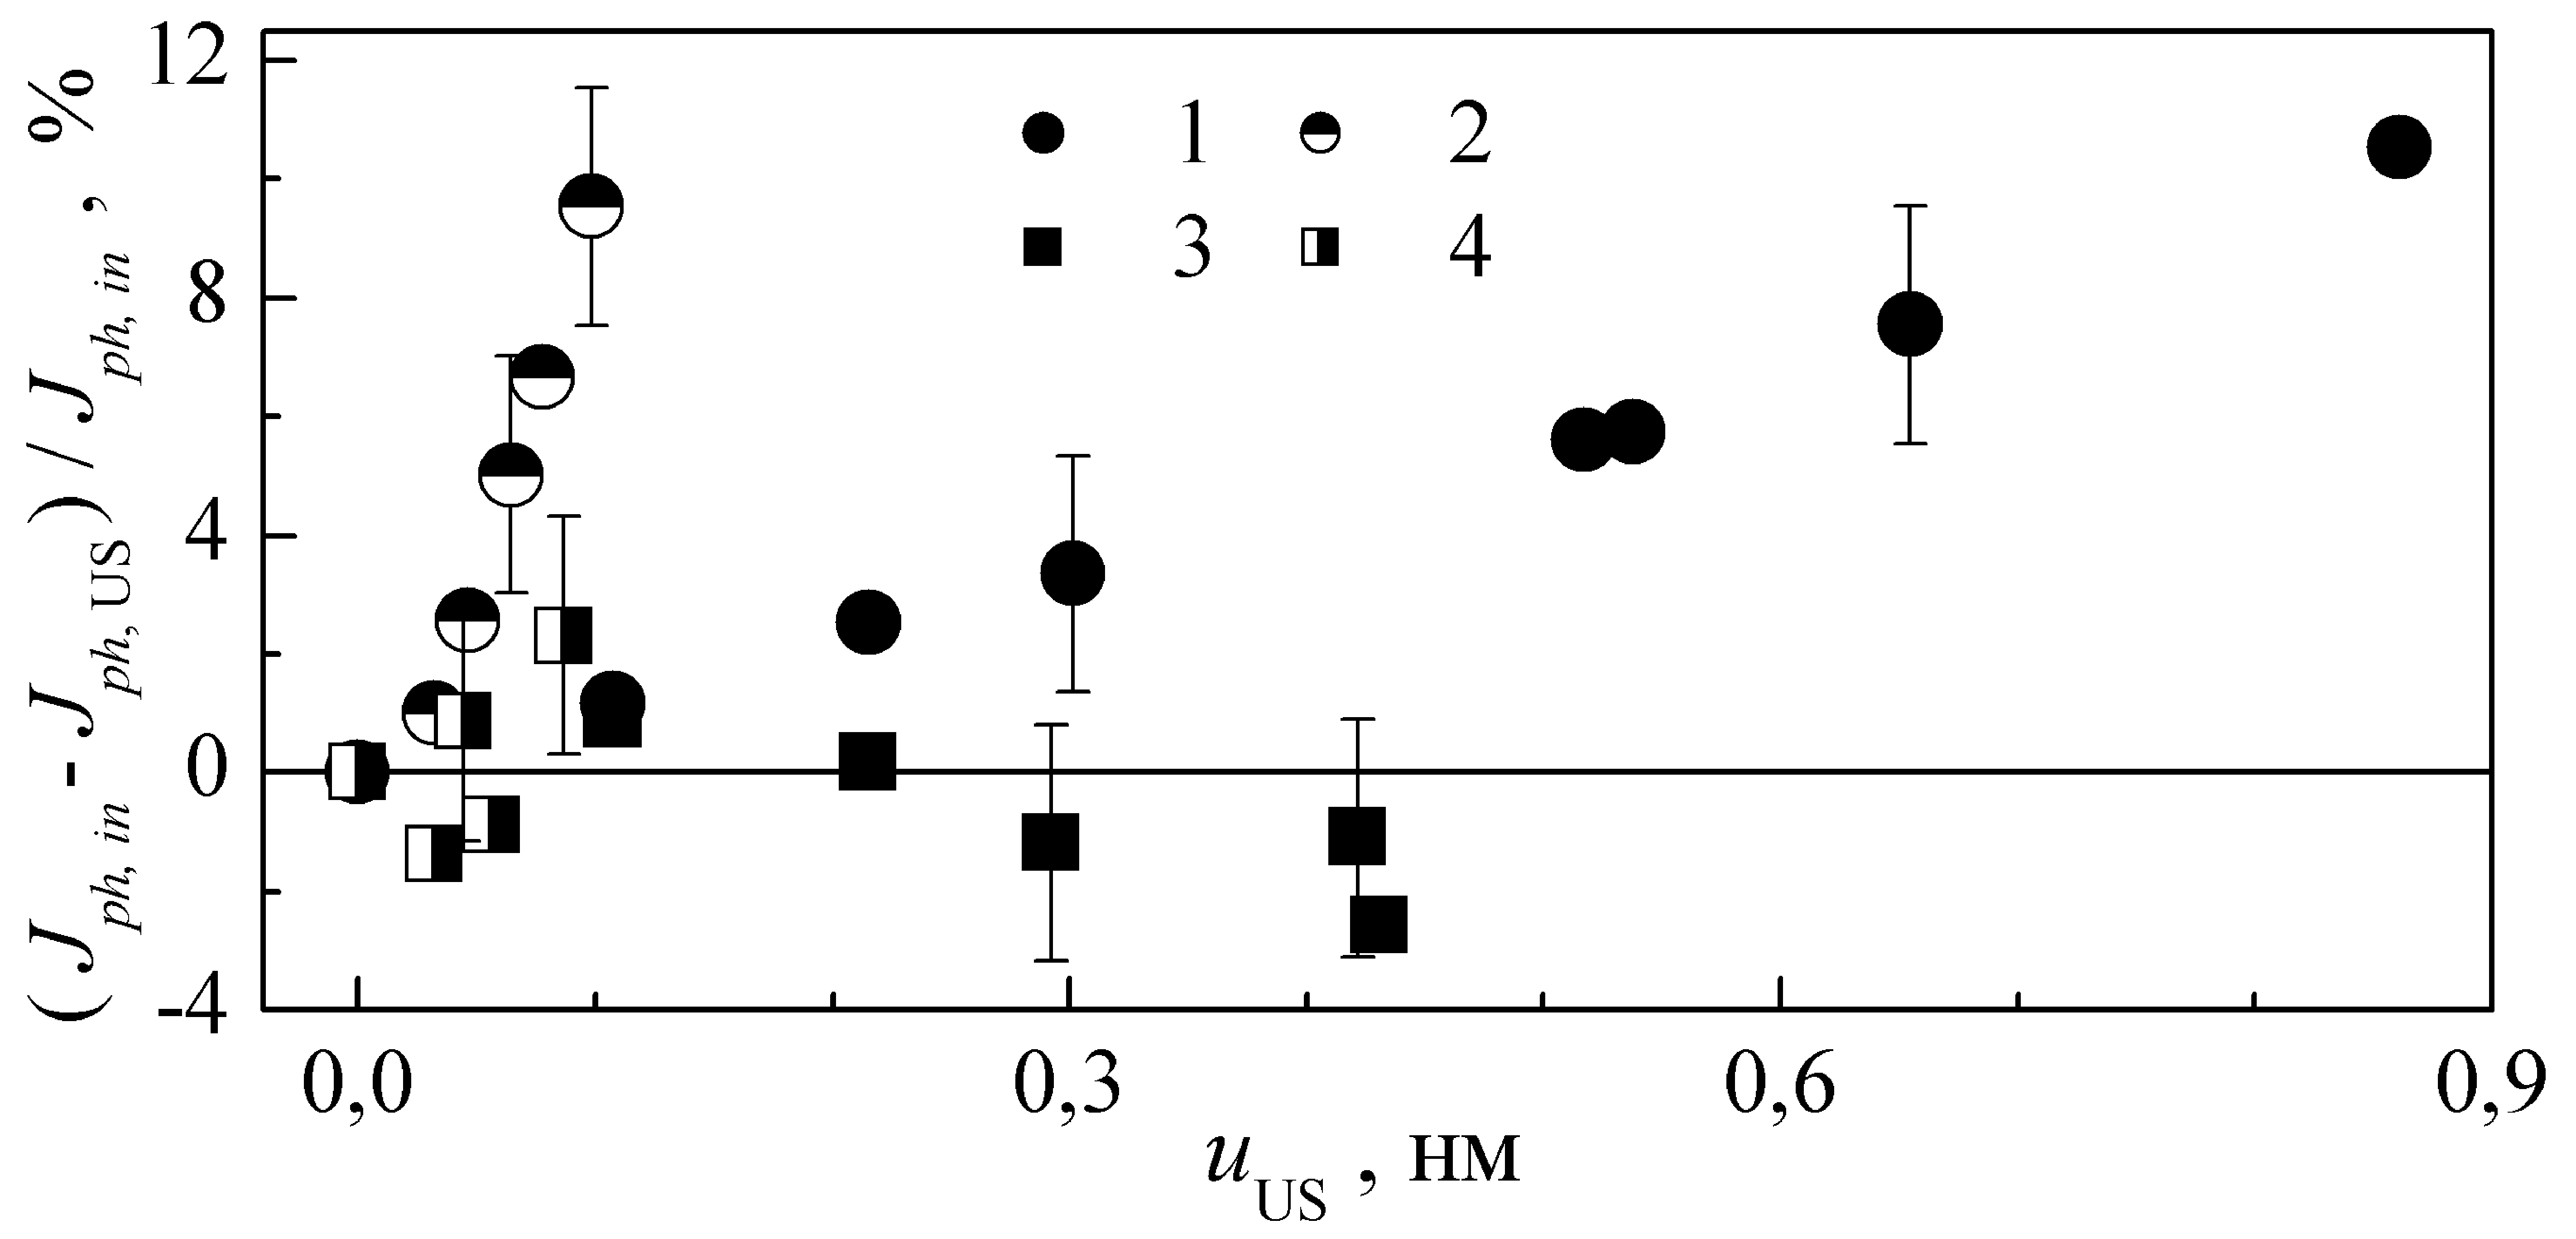
\includegraphics[width=0.6\textwidth]{figeIscRD}
\caption{\label{figeIscRD}
Залежності акустоіндукованих зменшення фотоструму від
амплітуди зміщень атомів в неопроміненому (1, 2)
та нейтронно--опроміненому (3, 4) зразках.
$f_\mathtt{US}$, Гц: 8,0 (1, 3);
26,1 (2, 4)
}%
\end{figure}
Виявлено, що УЗН $\gamma$--опромінених структур, як і вихідних, викликає зменшення величини $J_{ph}$, що цілком
узгоджується з виявленим акустоіндукованим підвищенням активності рекомбінаційних центрів (зменшенням $\tau_n$).
Водночас у нейтронно--опромінених зразках зміни $J_{ph}$ практично не спостерігаються --- рис.~\ref{figeIscRD}.
Дослідження температурних залежностей $J_{ph}$ та довжини дифузії неосновних носіїв заряду $L_n$,
засвідчило наявність у нейтронно--опромінених структурах додаткового механізму (ймовірно --- акустоіндукована зміна заселеності рівнів, пов'язаних з вакансійними кластерами, що викликає зменшення коефіцієнта відбивання) впливу УЗН.

Отримані   результати  підтверджують  практичну перспективність динамічного акустичного керування характеристиками напівровідникових приладів.


У  \underline{\textbf{третьому розділі}} наведено результати порівняльного аналізу та оптимізації методів розрахунку параметрів (струму насичення  $I_s$, висоти бар'єру Шотткі  $\Phi_b$, фактора неідеальності та послідовного опору) структур метал--напівпровідник з вольт--амперних характеристик в наближенні термоелектронної емісії (ТЕ):
\begin{eqnarray}
\label{eqSDIV}
\nonumber I&=&I_s\left\{\exp\left[\frac{q(V-IR_s)}{n_\mathrm{id}kT}\right]-1\right\}=\\
&=&AA^*\,T^2\exp\left(-\frac{q\Phi_b}{kT}\right)\left\{\exp\left[\frac{q(V-IR_s)}{n_\mathrm{id}kT}\right]-1\right\}\,,
\end{eqnarray}
де
$A$ --- площа діода Шотткі,
$A^*$ --- ефективна стала Річардсона.
%Увага була зосереджена на визначенні струму насичення  $I_s$, висоти бар'єру Шотткі  $\Phi_b$), фактора неідеальності та послідовного опору з ВАХ, яка при переважанні термоелектронної емісії (ТЕ), має описуватися виразом
Були розглянуті 10 аналітичних методів (використовують інтегрування ВАХ (метод Kaminski І), побудову різноманітних допоміжних функцій (чи їх масиву) та лінійну (методи Chung, Lee та Kaminski ІІ) чи нелінійну (Gromov) апроксимацію або пошук екстремумів (Cibils);
також для побудови функцій застосовують додаткові параметри (методи Norde та Bohlin) або диференційні коефіцієнти першого (Werner) або вищого порядків (Mikhelashvili))
2 числові методи (метод найменших квадратів зі статичними ваговими коефіцієнтами застосовувався безпосередньо до рівняння~(\ref{eqSDIV}) та до його розв'язку, вираженого через $W$--функцію Ламберта) та
4 еволюційних алгоритми (диференційної еволюції (DE),
оптимізації зграї частинок (PSO),
модифікованої штучної бджолиної сім'ї (MABC) та
оптимізованого викладання та навчання (TLBO)).
Всі методи були застосовані до
а)~ВАХ, синтезованих за допомогою виразу~(\ref{eqSDIV});
б)~ВАХ, синтезованих за допомогою виразу~(\ref{eqSDIV}) з врахуванням можливих випадкових похибок вимірювань;
в)~експериментально виміряних ВАХ кремнієвих діодів Шотткі.

Для методів Norde та Bohlin визначені  оптимальні (для кремнієвих діодів Шотткі при вимірюваннях в діапазоні температур $130\div330$~К) величини додаткових параметрів (1,8 для Norde та 1,6 і 3,5 для Bohlin).
Запропоновано модифікацію методу Mikhelashvili, яка дозволяє застосовувати його в автоматичному режимі до множини ВАХ;
вона полягає у послідовному використанні медіанного фільтру та процедури згладжування функції $\alpha(V)=d(\ln I)/d(\ln V)$ перед визначенням положення її максимуму;
показано доцільність застосування запропонованої процедури при опрацюванні реальних ВАХ для підвищення точності методу.
Запропоновано адаптивну процедуру вибору діапазону ВАХ, який використовується для побудови допоміжних функцій при застосуванні аналітичних методів визначення параметрів та показано, що вона дозволяє підвищити точність визначення параметрів (приблизно на порядок при кімнатних температурах у випадку низького рівня похибок вимірювання) і не викликає критичного збільшення часу розрахунку.

\begin{table}[t]
\caption{\label{tabRT}Час визначення параметрів діодів Шотткі}
\centering
\begin{tabular}{|r|c|r|c|}
\hline
\multicolumn{1}{|c|}{Метод}&Час роботи, с &\multicolumn{1}{c|}{Метод}&Час роботи, с\\ \hhline{|====|}
Norde &$(2,6\div3,7)\cdot10^{-5}$& Werner  &$(4,0\div4,5)\cdot10^{-5}$\\ \hline
Cibils  &$(0,2\div5,3)\cdot10^{-3}$& Kaminskii I &$(4,5\div8,0)\cdot10^{-5}$\\ \hline
Kaminskii II &$(0,3\div2,6)\cdot10^{-3}$& Bohlin &$(4,0\div6,3)\cdot10^{-5}$\\ \hline
Lee &$(0,2\div3,6)\cdot10^{-3}$& Gromov &$2.2\cdot10^{-2}$\\ \hline
Cheung &$(2,0\div3,2)\cdot10^{-5}$&Mikhelashvili &$(2,9\div4,7)\cdot10^{-5}$\\ \hline
Ordinary LS &$1,8\div460$&Lambert LS &$7,6\div540$\\ \hline
DE &$0,36\div0,73$&PSO &$0,14\div0,35$\\ \hline
MABC &$5.7\cdot10^{-2}\div0,20$&TLBO &$5.4\div19,2$ \\
\hline
\end{tabular}
\end{table}

Виявлено, що
а)~відносні похибки визначення $R_s$, $\Phi_b$ та $n_\mathrm{id}$ лінійно залежать як від величин відносних похибок вимірювання напруги, так і сили струму, причому в останньому випадку залежність слабша;
б)~помилки визначення $\Phi_b$ та $n_\mathrm{id}$ значно менші, ніж помилки визначення $R_s$ за тих самих умов вимірювання.
Проведено порівняльний аналіз точності (рис.~\ref{figId} та \ref{figPrAcc}) та швидкодії (табл.~\ref{tabRT}) визначення параметрів різними методами.
Показано, що найбільша точність досягається при використанні еволюцiйних алгоритмів, числових методів, методу Gromov з адаптивною процедурою та методу Lee.
Використання функції Ламберта при застосуванні числових методів дозволяє зменшити помилки визначення параметрів.
Визначено вплив абсолютних величин кожного з параметрів на точність визначення $R_s$, $\Phi_b$ та $n_\mathrm{id}$.
Зокрема показано, що еволюційні алгоритми дозволяють отримати найбільш коректні результати при малих (декілька Ом) значеннях $R_s$ або високих температурах, а найбільш стійкими до величин параметрів є точності числових методів.
\begin{figure}[ht]
\center
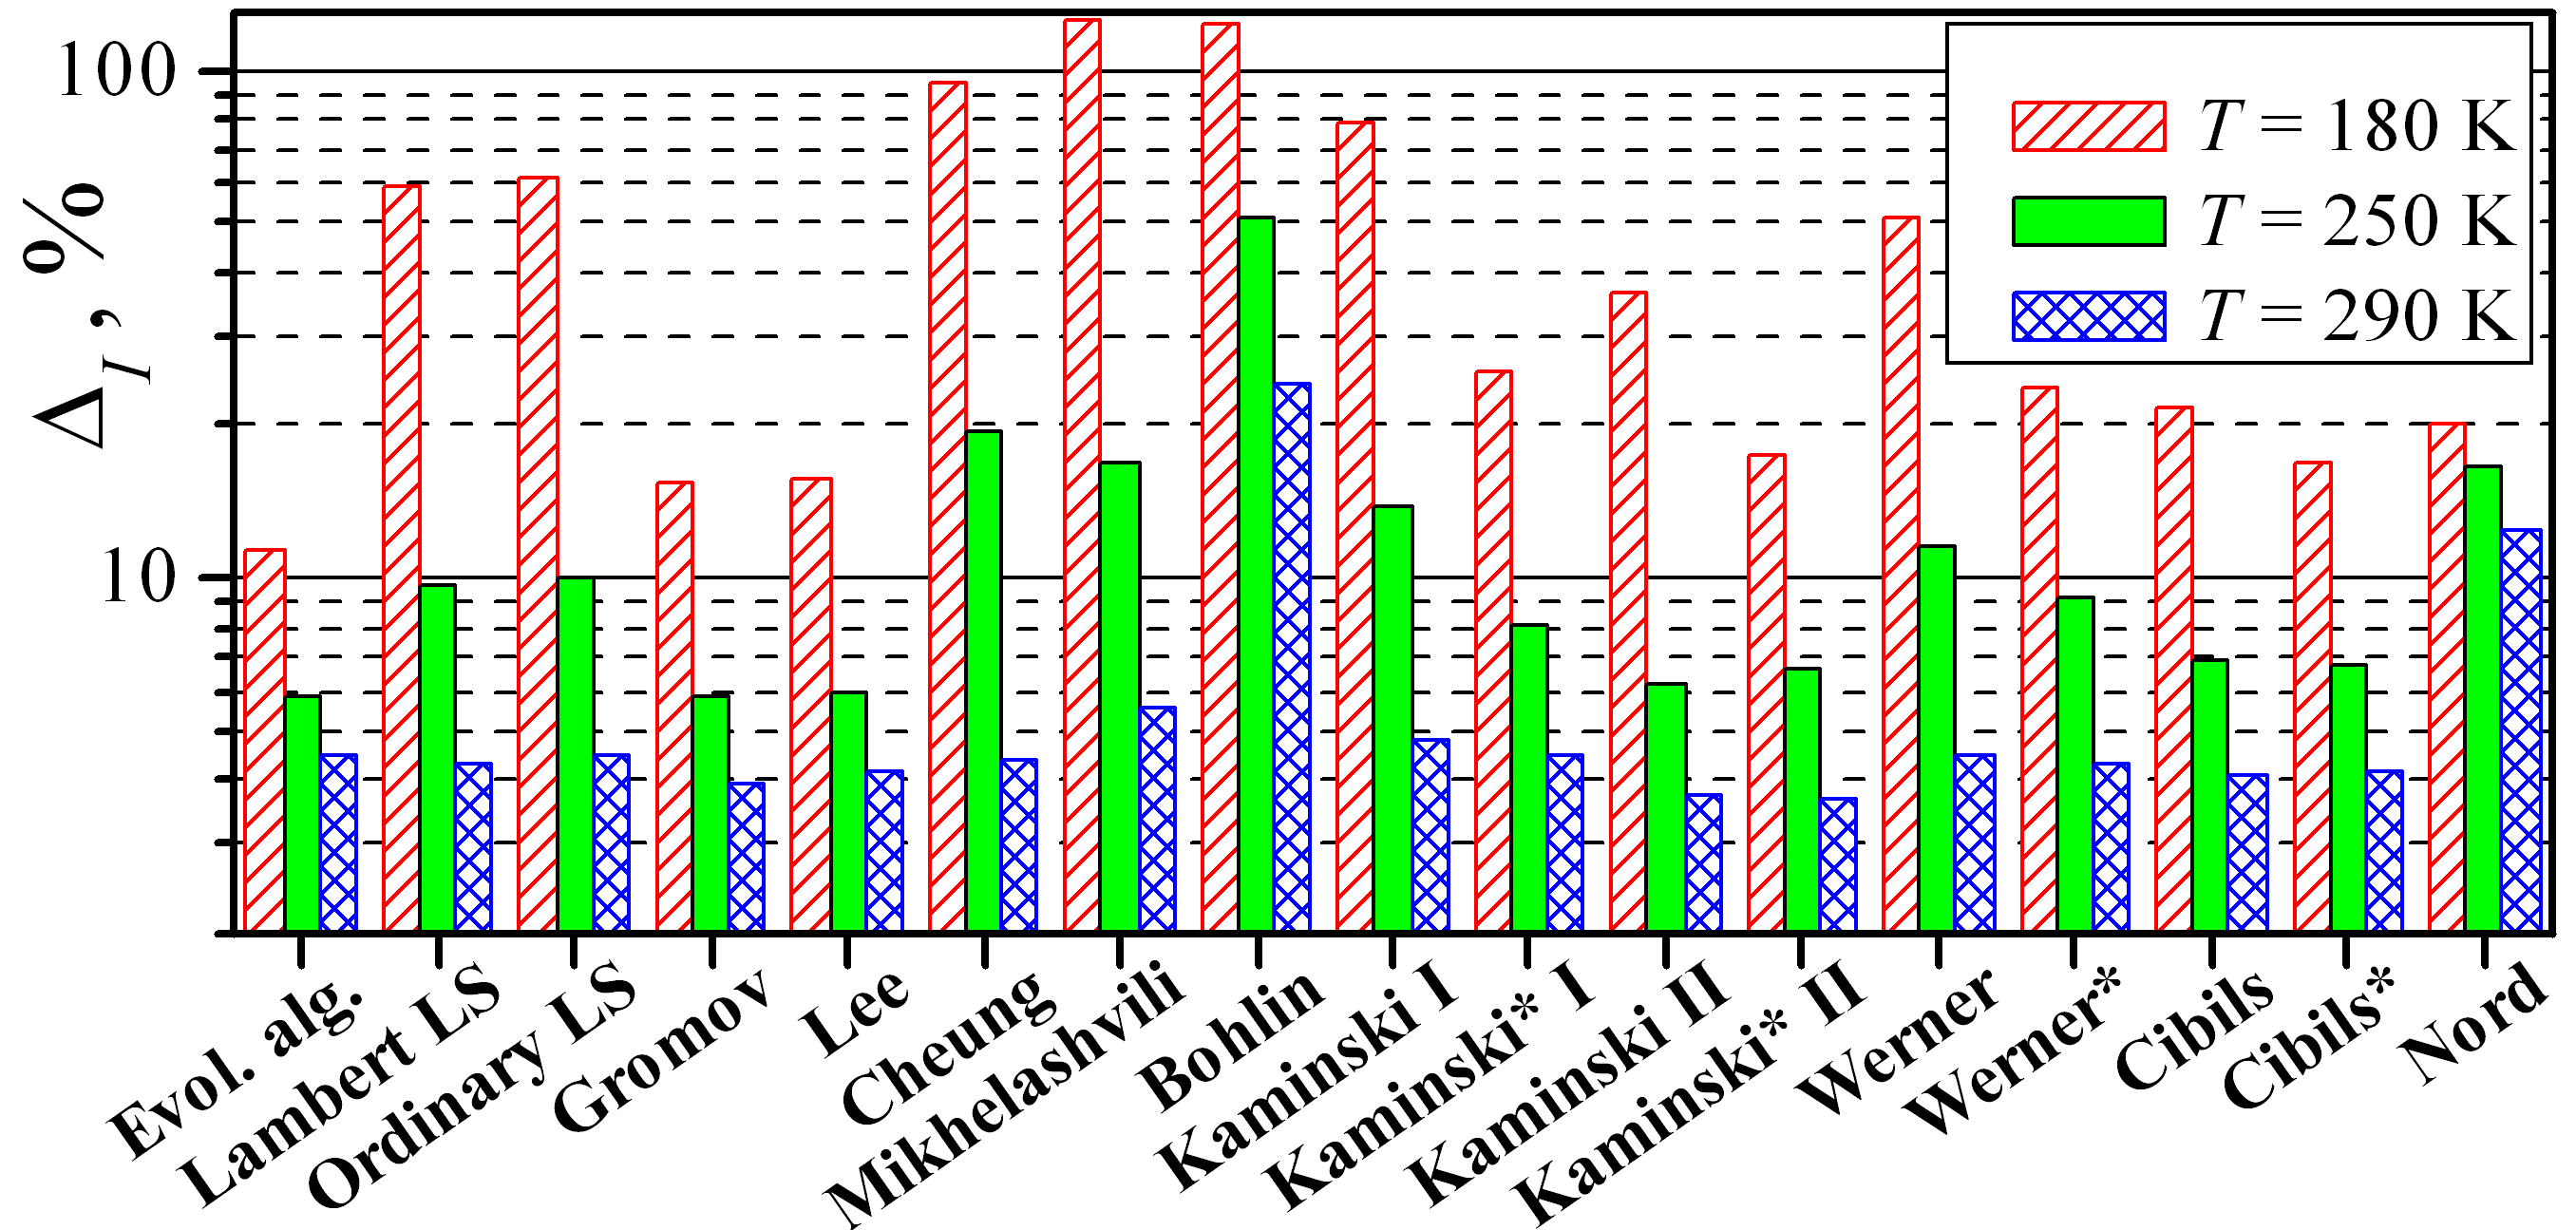
\includegraphics[width=0.8\textwidth]{figPrAcc}%
\caption{\label{figPrAcc}
Середні значення відносного відхилення розрахованих значень сили струму від експериментальних даних
}
\end{figure}

\begin{figure}
\center
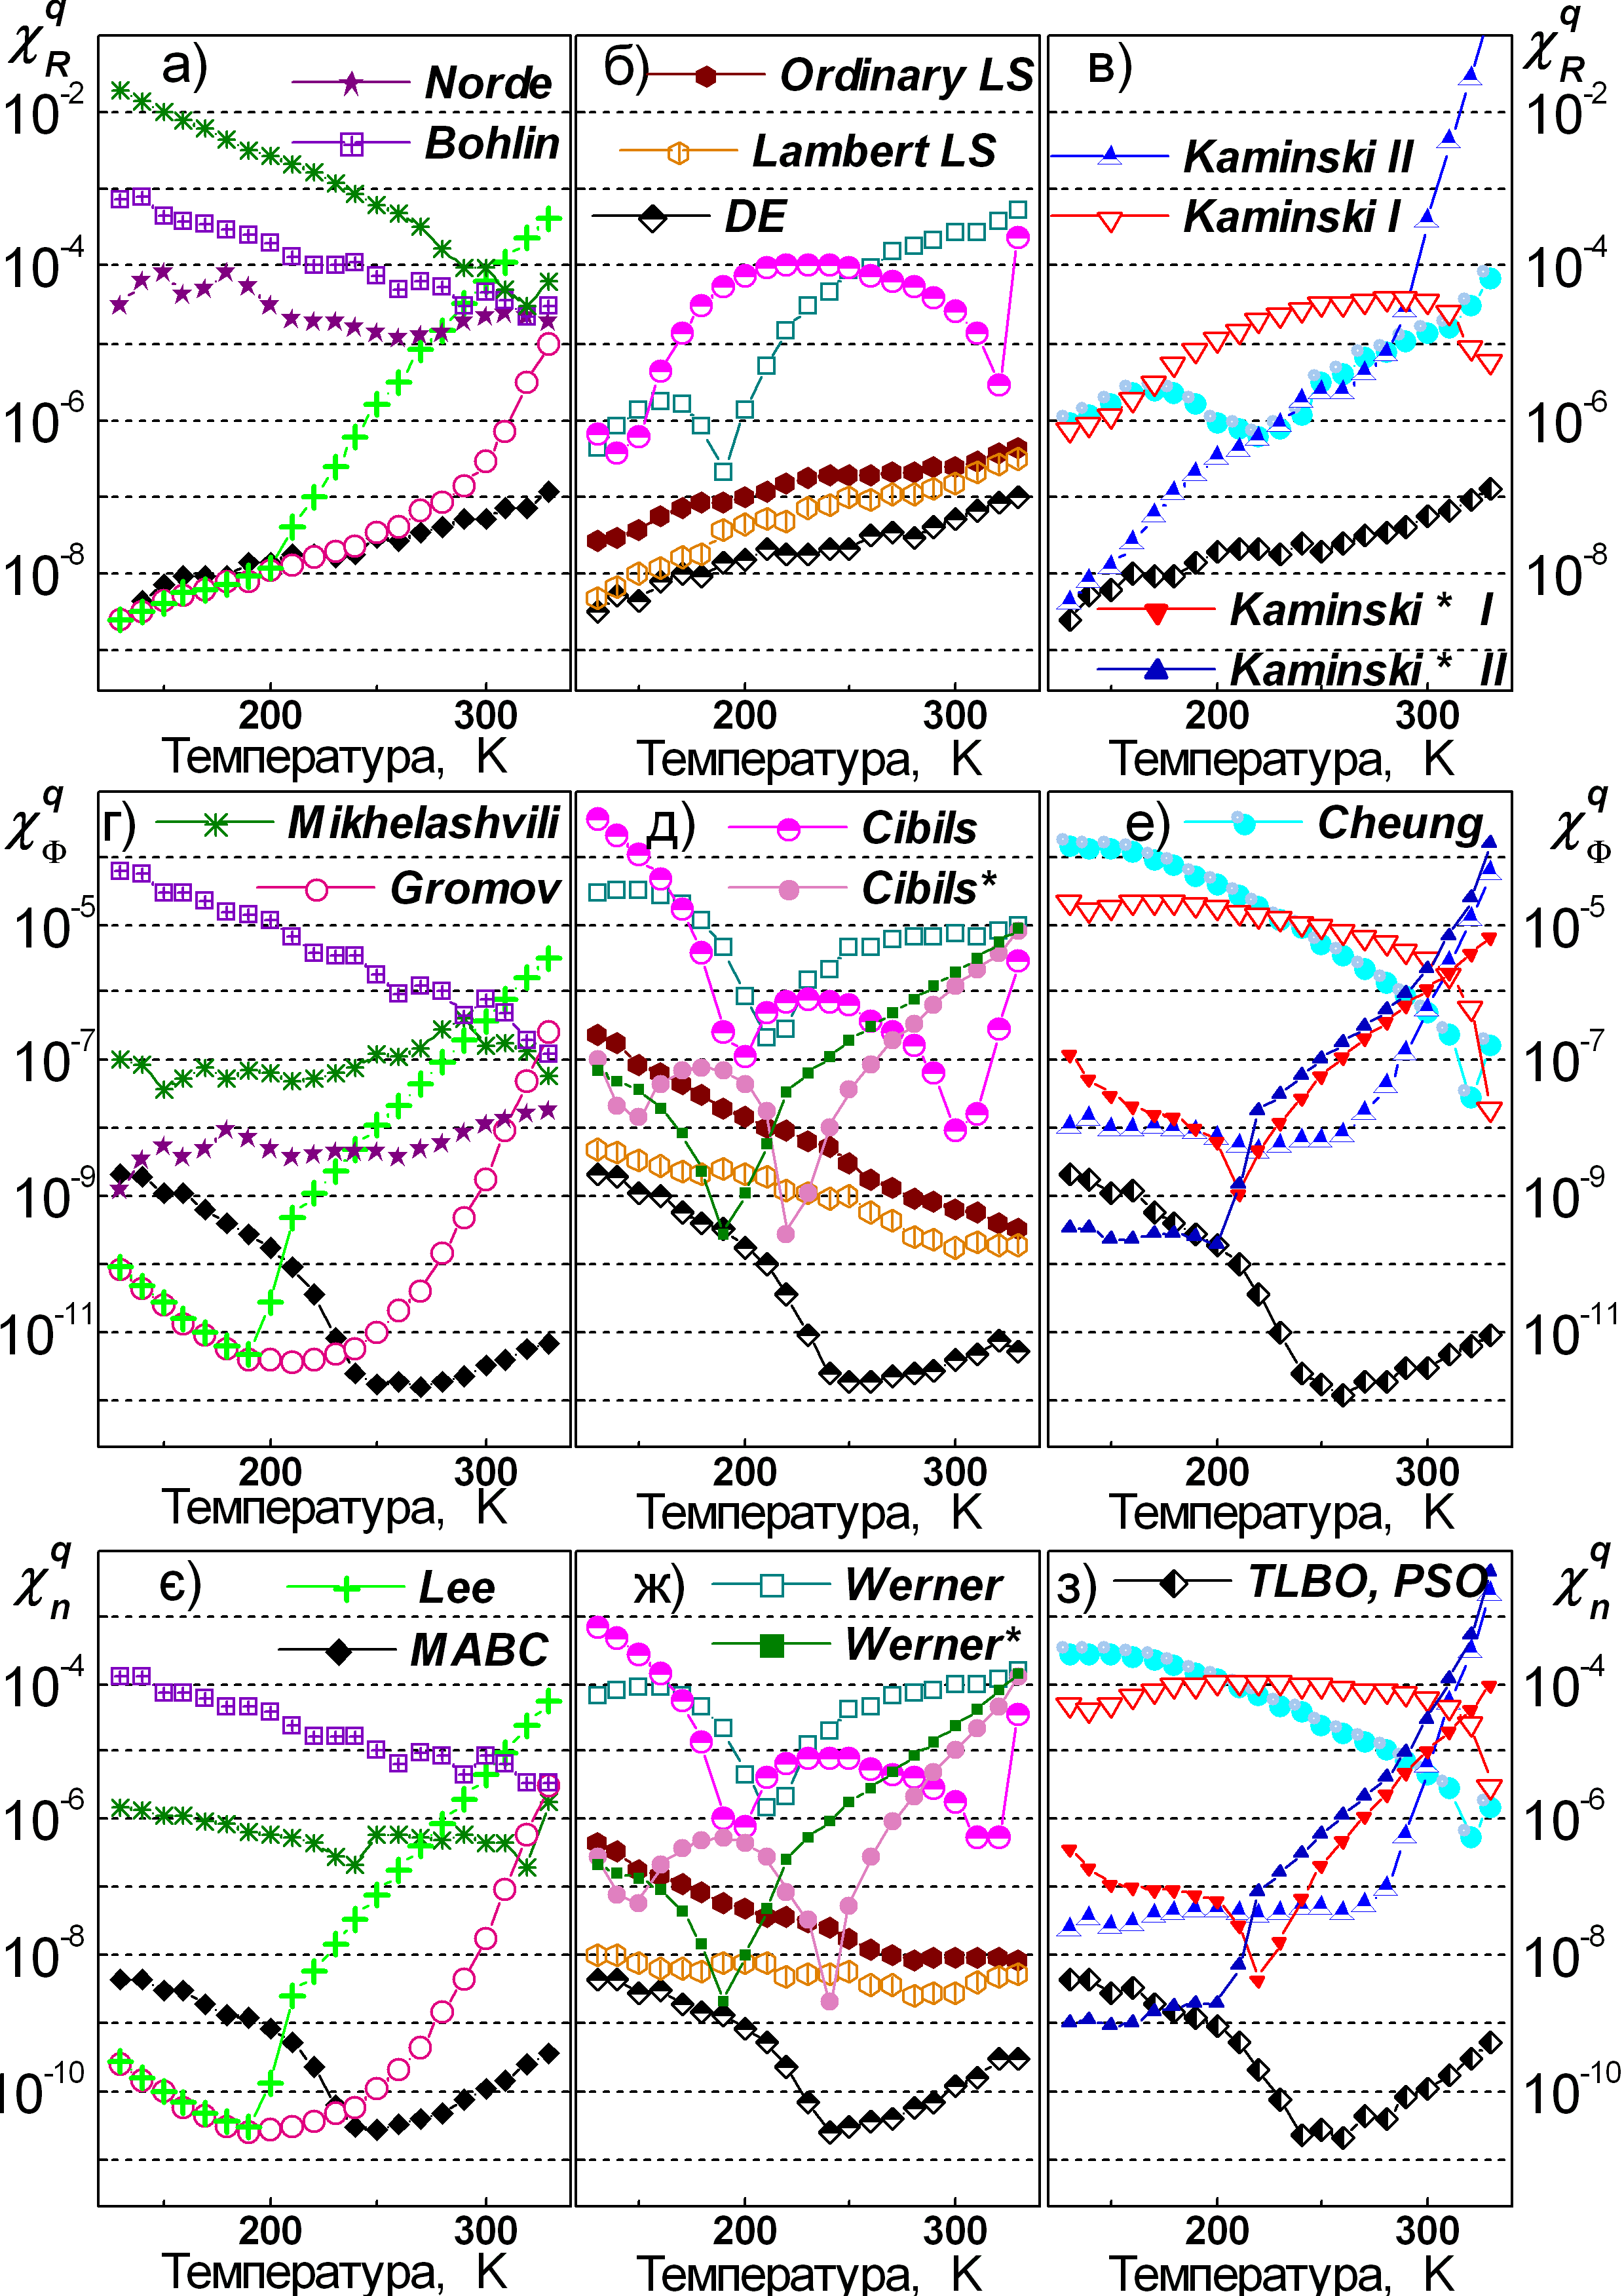
\includegraphics[width=0.75\textwidth]{figId}%
\caption{\label{figId}
Температурні залежності відносних похибок визначення $R_s$ (а --- в), $\Phi_b$ (г --- е) та $n_\mathrm{id}$ (є --- з) при застосуванні методів до синтезованих ВАХ
}
\end{figure}




Важливо підкреслити, що представлені результати огляду, тестування та порівняльного аналізу методів визначення параметрів діодів Шотткі можуть бути корисними під час досліджень та розробок пристроїв з контактом метал--напівпровідник на базі не лише кремнію, але й інших напівпровідників.


У  \underline{\textbf{четвертому розділі}} представлені результати досліджень
впливу $\gamma$--опромінення на структури Al---$n$--$n^+$--Si з контактом Шотткі та
вперше виявлених динамічних акустоіндукованих ефектів в цих структурах при кімнатних температурах.

Встановлено, що поява при низьких ($T<210$~К) температурах додаткової компоненти прямого струму,
а також температурні залежності висоти бар'єру та фактору неідеальності можуть бути пояснені
з точки зору моделі ТЕ через неоднорідний контакт
%\cite{Tung:MSE}
[5$^*$].
%
%Виявлено, що для неопромінених структур спостерігається поява при низьких ($T<210$~К) температурах додаткової компоненти струму,
%збільшення ВБШ при зростанні температури (рис.~\ref{figFbTrad_SDA}) та зменшення фактора неідеальності:
%\begin{equation}\label{eqN_T:TE}
%n_{\mathrm{id}}=1+\frac{T_0}{T},
%\end{equation}
%де $T_0=12$~K.
%Показано, що всі виявлені особливості можна пояснити з точки зору моделі ТЕ через неоднорідний контакт
%%\cite{Tung:MSE}
%[5$^*$].
%Про це свідчать лінійність залежностей $\Phi_{b}$ та $(n_{\mathrm{id}}^{-1}-1)$ від $q/2kT$, $\Phi_{b}$ від $n_{\mathrm{id}}$,
%збіг експериментально визначеного значення $T_0$  та відомого з літератури значення $A^*$ (112~А$\cdot$см$^{-2}\cdot$К$^{-2}$) з відповідними величинами,
%розрахованими в рамках цієї моделі на основі температурної залежності ВБШ.
       Визначені середня висота бар'єру Шотткі $\Phi_b^0$ та її стандартне відхилення $\sigma_{\Phi}$:
       $0,872\pm0,004$~В та $0,099\pm0,001$~В при $(130\div220)$~К та
       $0,663\pm0,003$~В та $0,040\pm0,005$~В при $(230\div330)$~К, відповідно.
Визначено середнє значення висоти бар'єру Шотткі в області зі зниженим бар'єром (так званого патчу) $54\pm4$~мВ.
Показано, що при зворотних зміщеннях струм $I_R$ складається з двох компонент --- рис.~\ref{figIVrg0USL_SDA},а.
Перша з яких, $I_\mathrm{TE}$, пов'язана з ТЕ процесами через неоднорідний контакт,
%:
%$I_\mathrm{TE}\sim T^2\exp(-E_\mathrm{TE}/kT)$,
%$E_\mathrm{TE}\sim V_R^{2/3}$,
%$V_R$ --- зворотна напруга.
%Друга,
тоді як друга,
$I_\mathrm{FN}$, викликана процесами тунелювання за участю
центру з енергетичним положенням $E_c-(120\pm5)$~меВ, пов'язаним, найімовірніше, з міжвузольним атомом вуглецю С$_i$.
%Внесок ТЕ складової зростає при підвищенні $T$ та зменшенні $V_R$.

\begin{figure}
\center
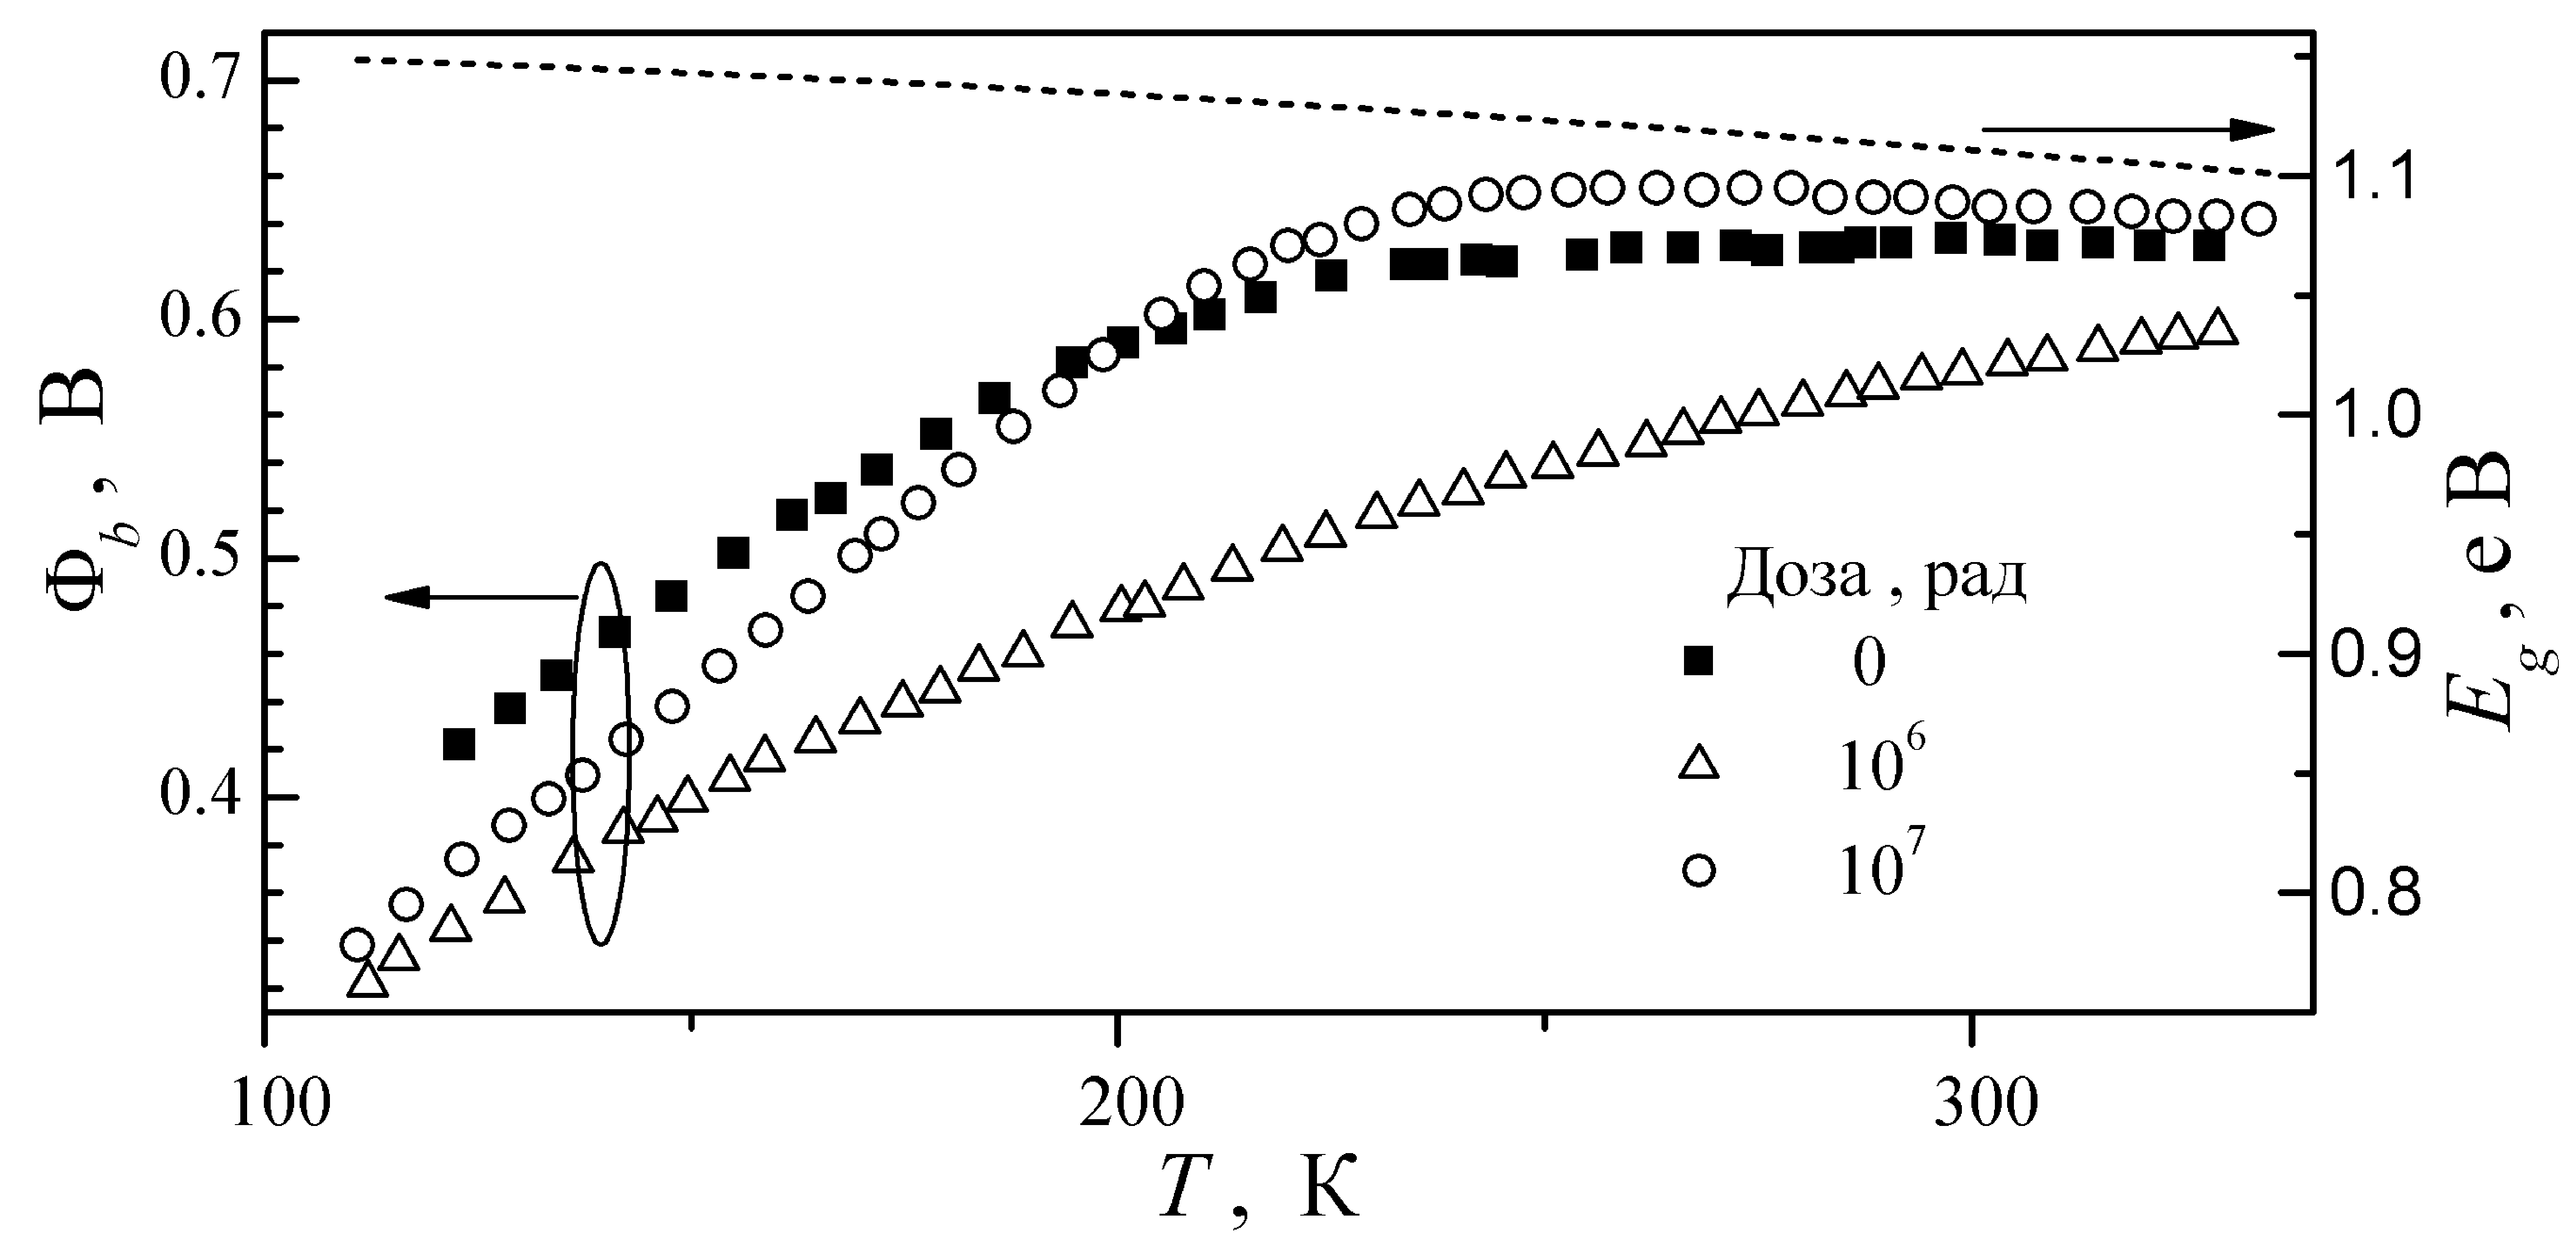
\includegraphics[width=0.7\textwidth]{figFbTrad_SDA}
\caption{\label{figFbTrad_SDA}
Температурні залежності висоти бар'єру структур Al---$n$--$n^+$--Si.
Пунктирна лінія --- залежність ширини забороненої зони кремнію
}%
\end{figure}



\begin{figure}[b]
\center
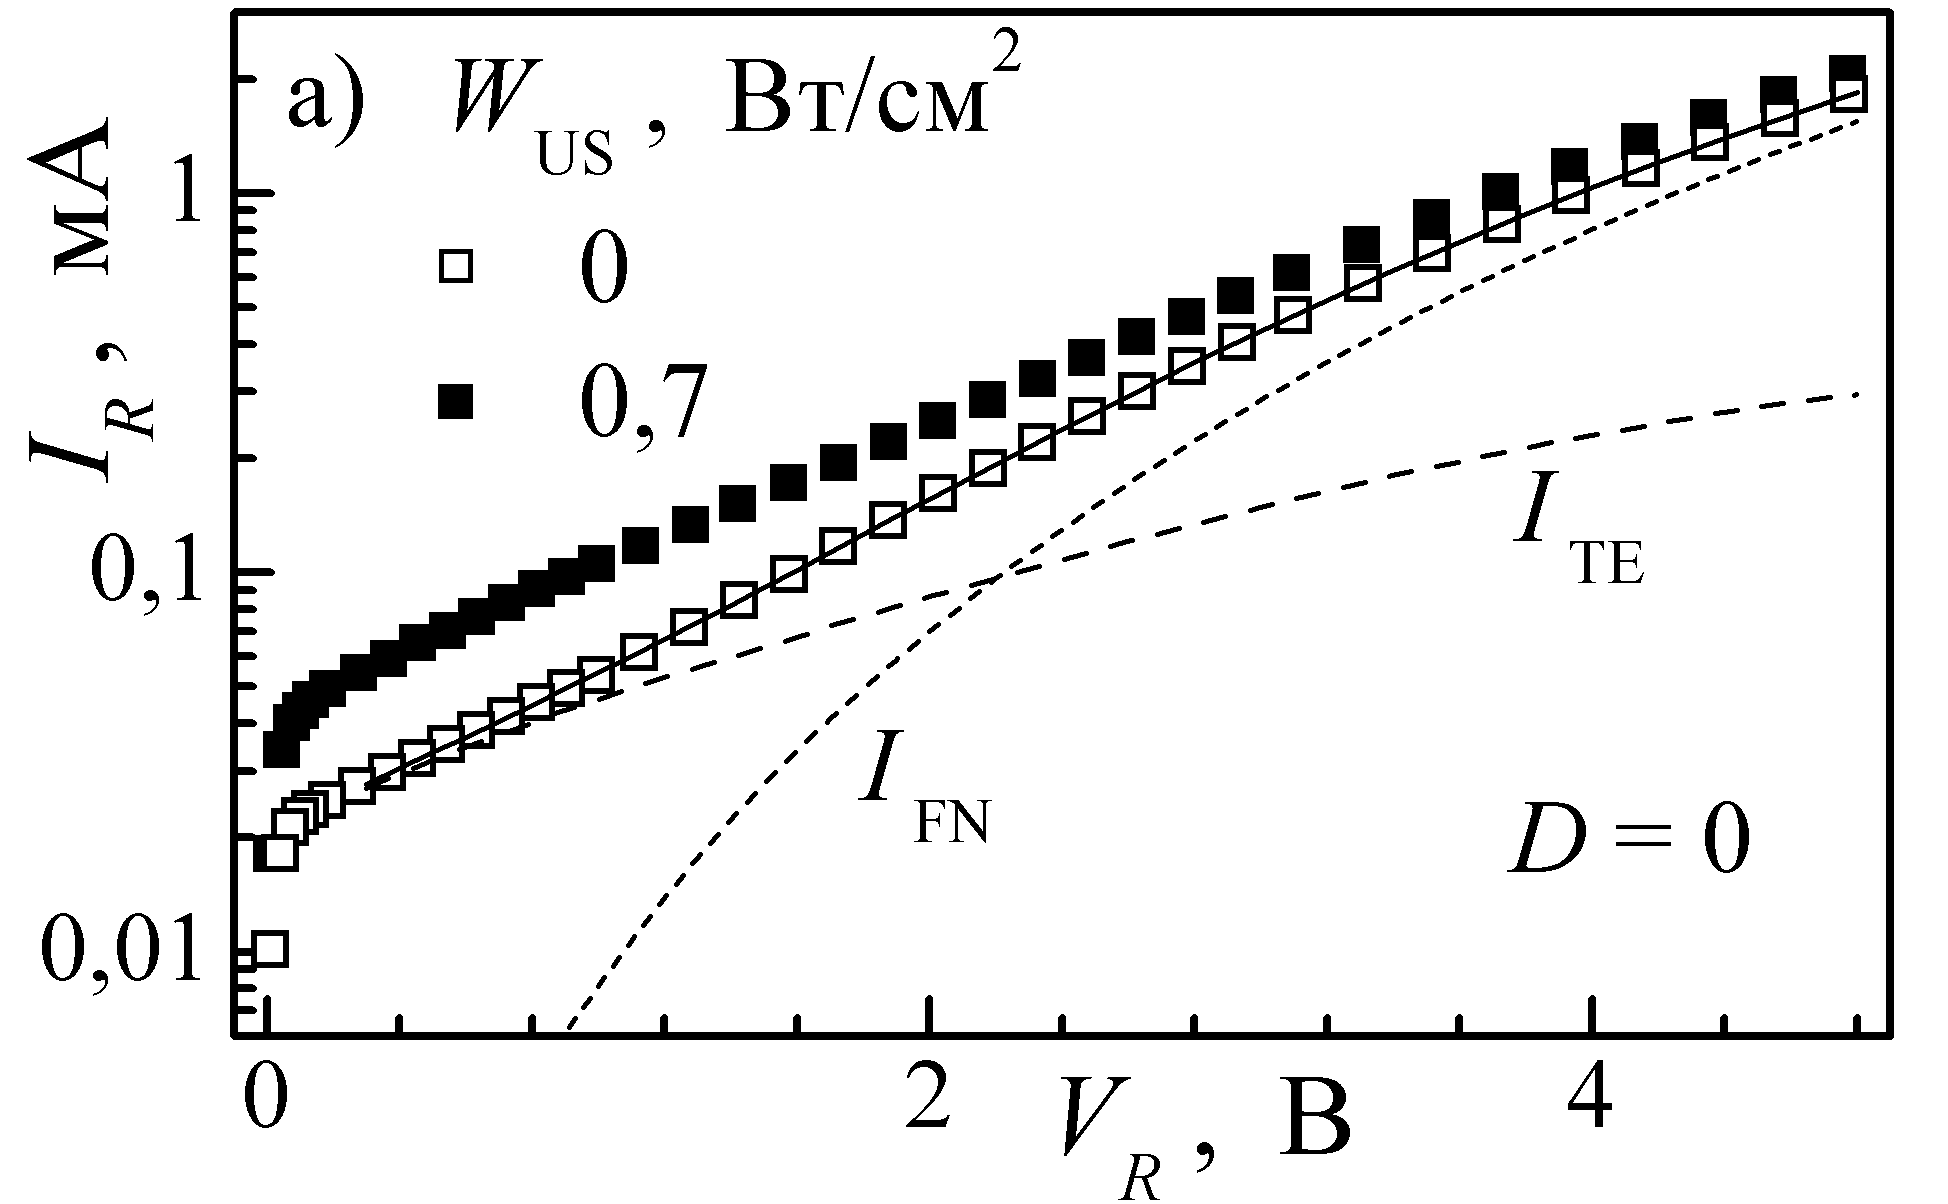
\includegraphics[width=0.33\textwidth]{figIVrg0USL_SDA}\hfill
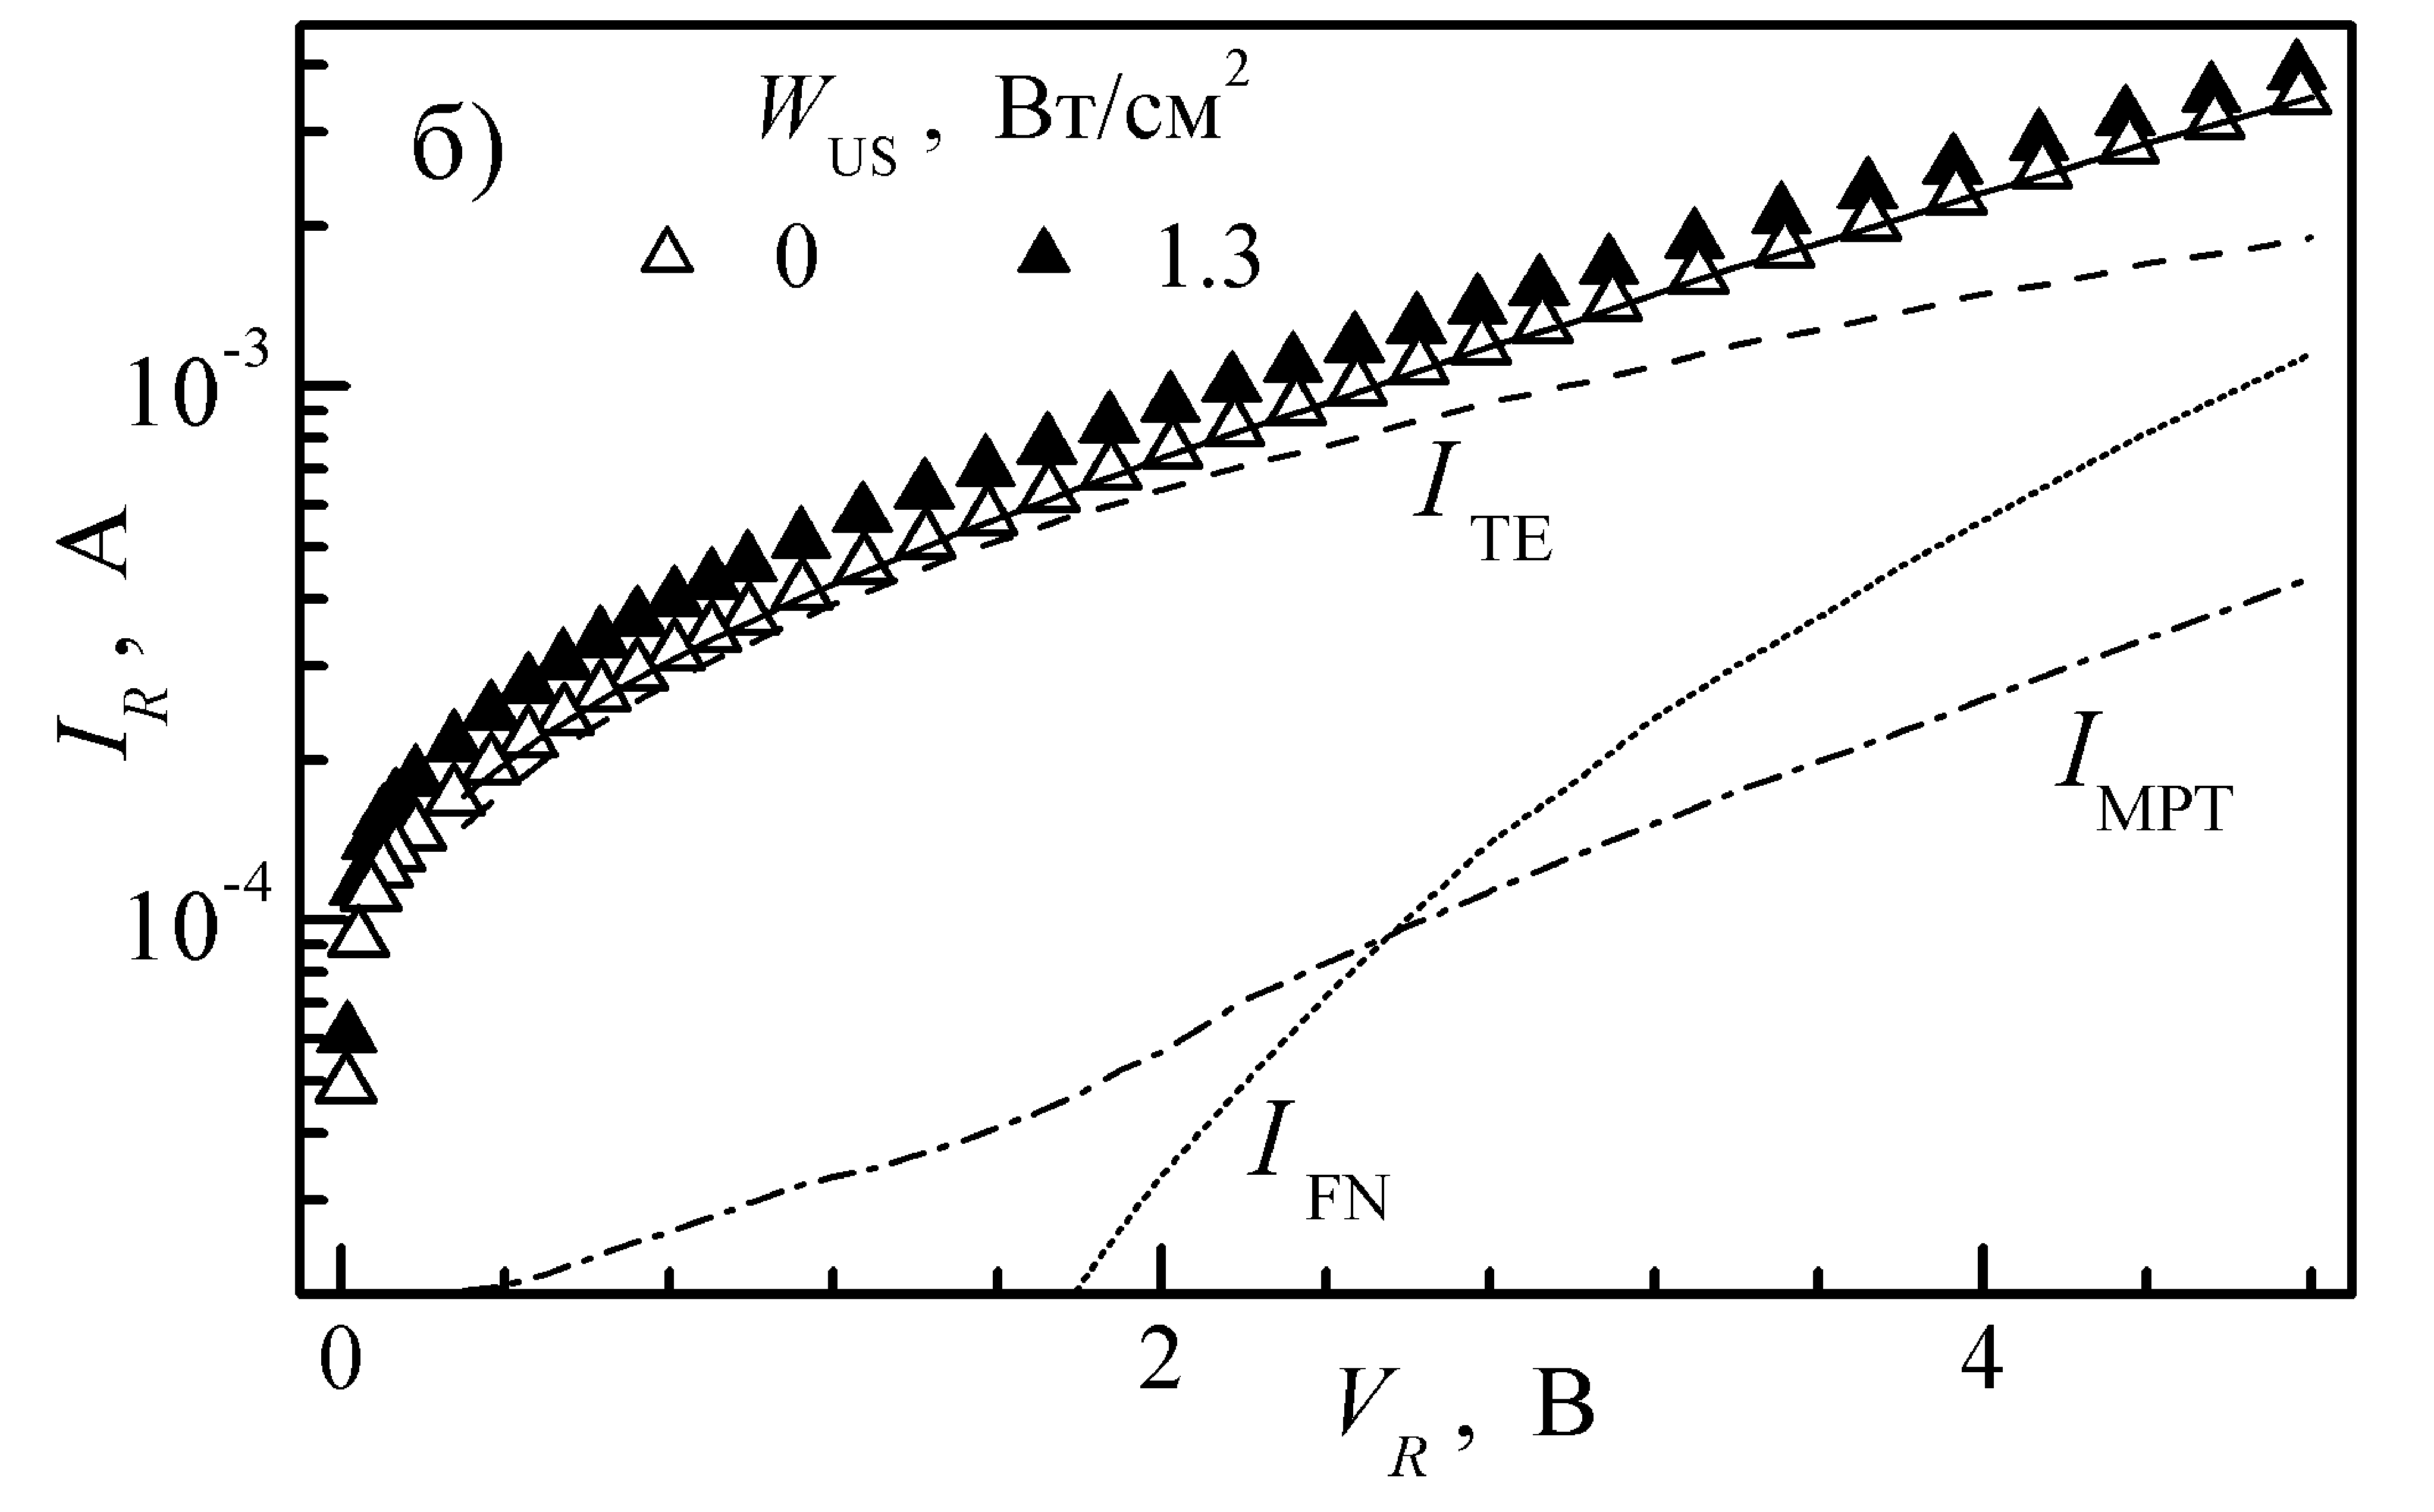
\includegraphics[width=0.33\textwidth]{figIVrg6USL_SDA}\hfill
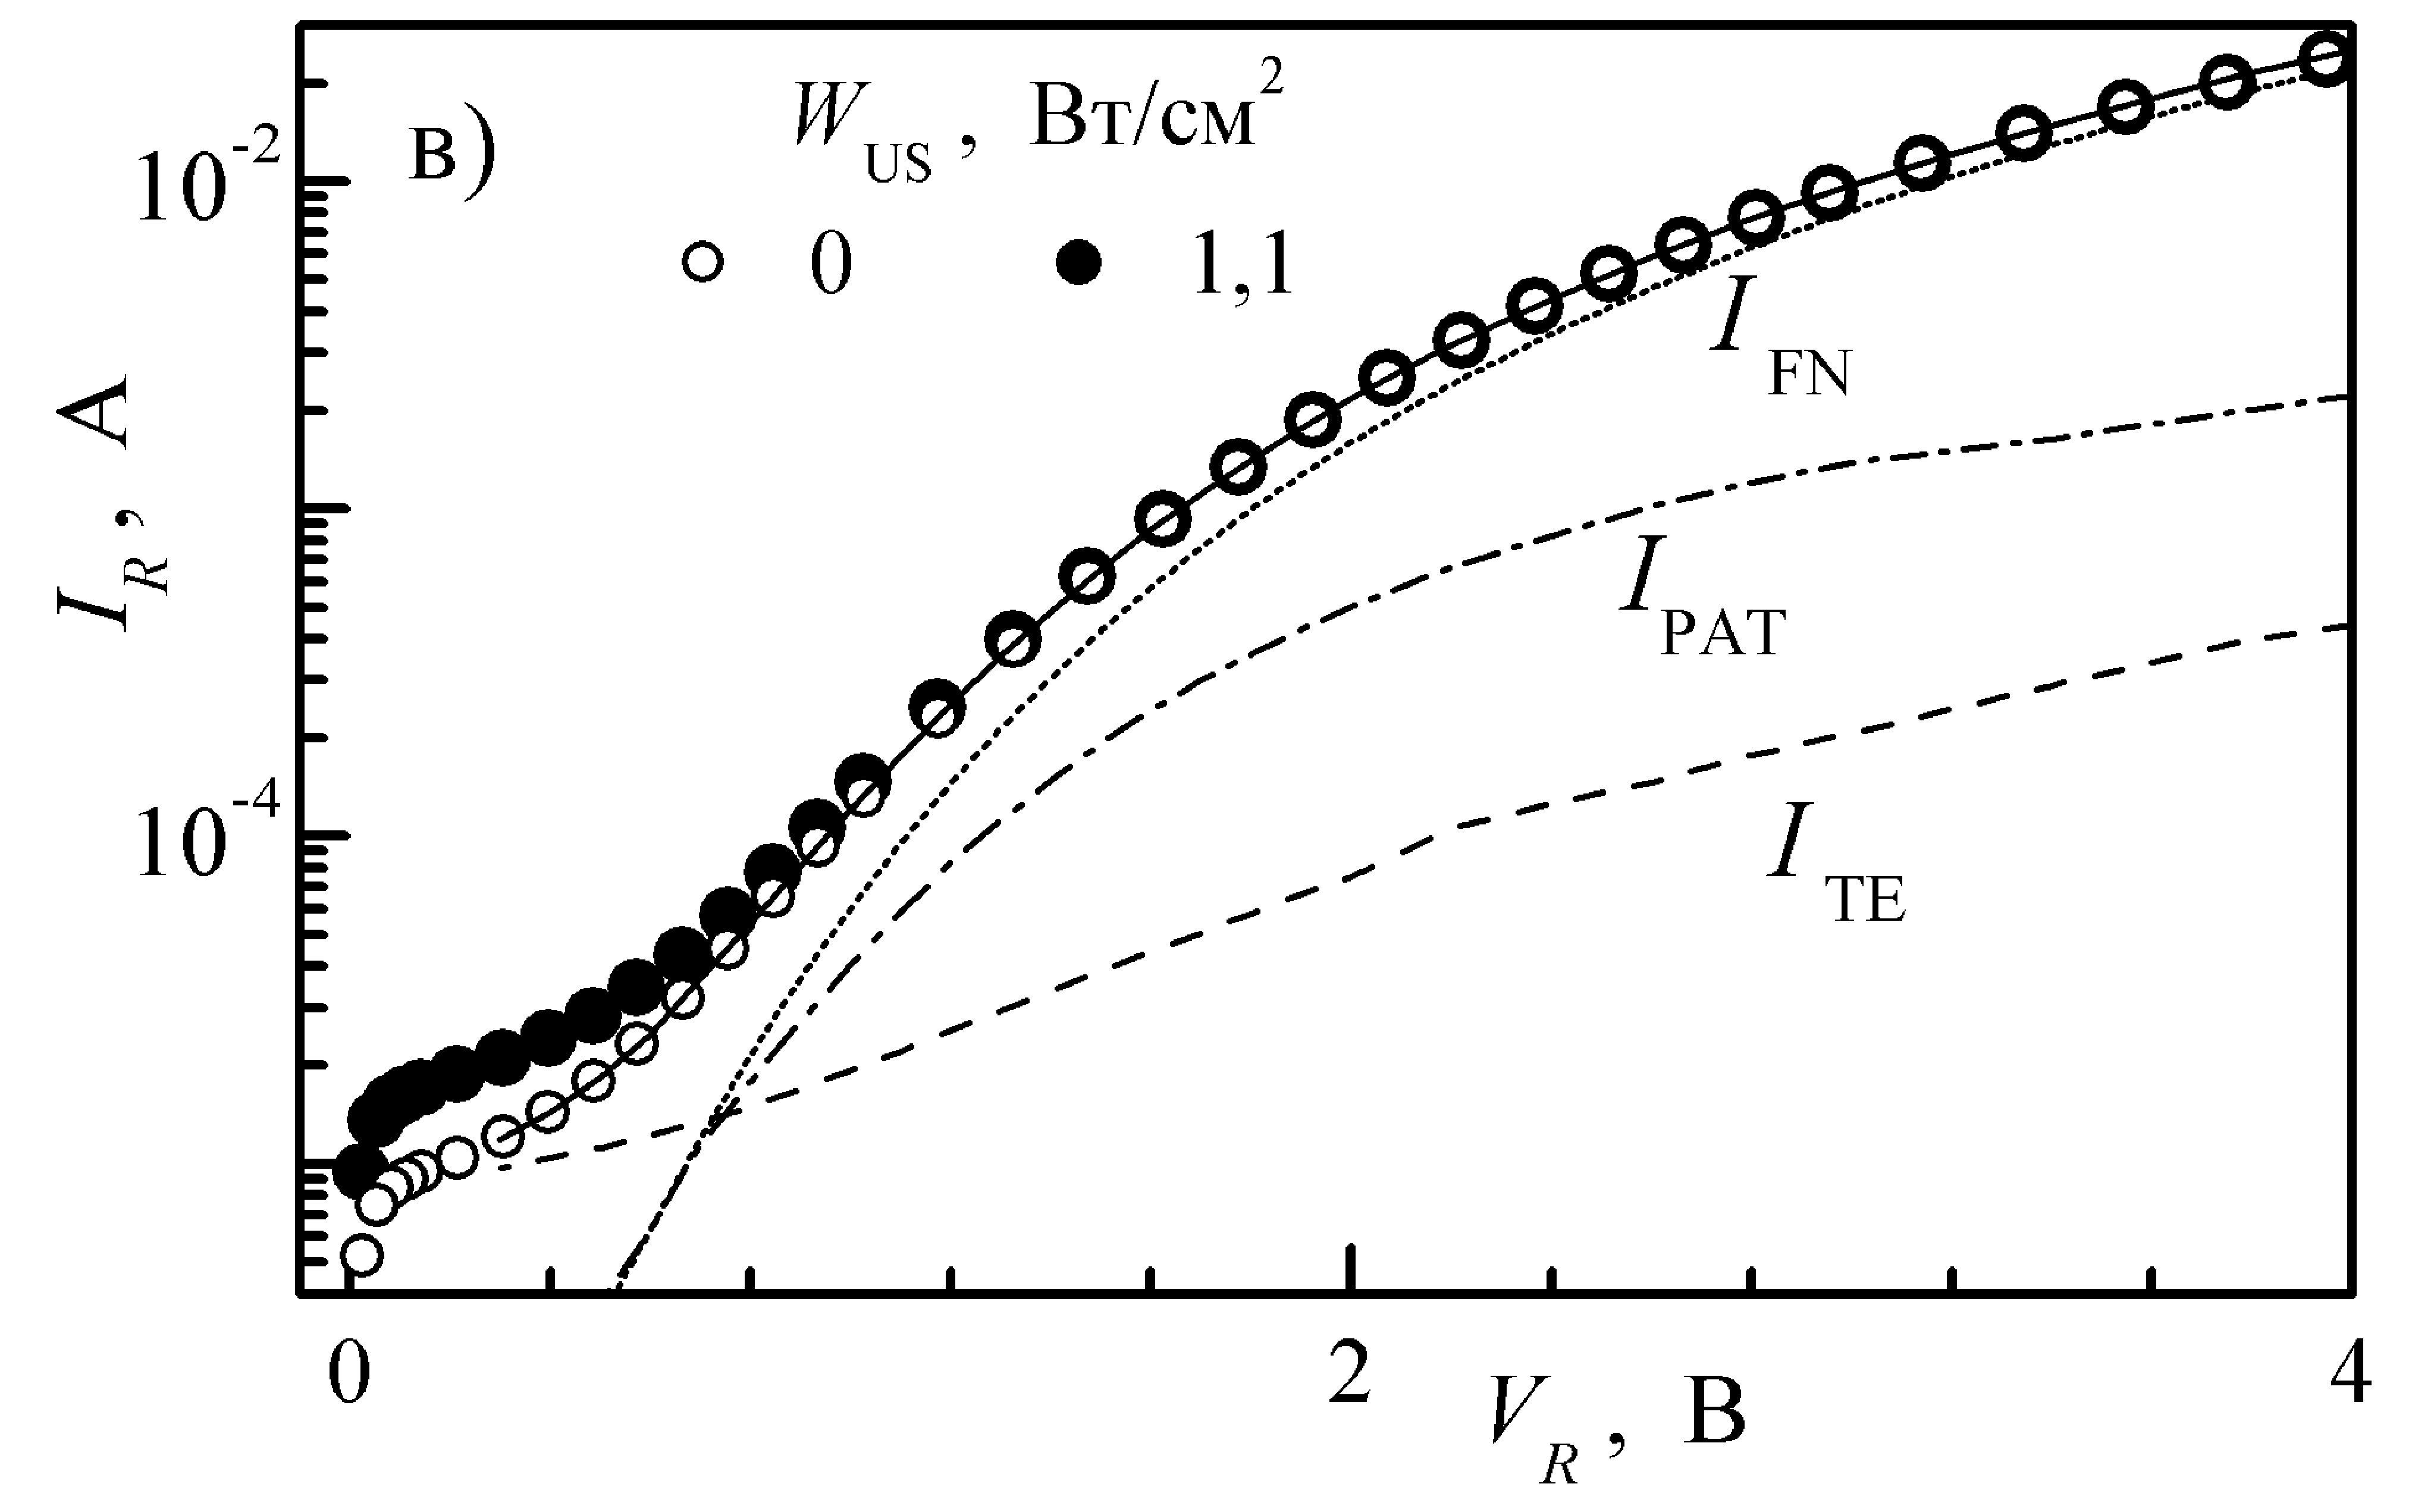
\includegraphics[width=0.33\textwidth]{figIVrg7USL_SDA}
\caption{\label{figIVrg0USL_SDA}
Зворотні  ВАХ  структур Al---$n$--$n^+$--Si з різним ступенем опромінення.
$T=305$~K.
Заповнені та порожні точки відповідають вимірам за умов УЗН та без нього, відповідно.
$f_\mathtt{US}=9,6$~МГц.
Розривні лінії відображають окремі складові зворотного струму для ненавантажених структур,
суцільні --- їх суму
}%
\end{figure}

Проведені дослідження показали, що при
опроміненні $\gamma$--квантами $^{60}$Co з дозами $D\!=\!10^6$~рад та $D\!=\!10^7$~рад відбувається
немонотонні зміни висоти бар'єра Шотткі --- рис.~\ref{figFbTrad_SDA}.
%Зауважимо, що в літературі повідомлялося подібні немонотонні дозові залежності $\Phi_{b}$, причому зустрічаються повідомлення про немонотонності двох типів (<<спад--зростання>> чи <<зростання--спад>>).
При зворотному зміщенні в опромінених структурах з'являється додаткова компонента струму, $I_\mathrm{MPT}$,
%внесок якої зростає з підвищенням дози.
%Температурні та польові залежності дозволили ідентифікувати $I_\mathrm{MPT}$ як струм,
пов'язана з тунельною багатофононною іонізацією глибоких домішкових центрів
%\cite{Ganichev:2000}
[6$^*$].
%Крім того, для структур з $D=10^7$~рад, на відміну від меншої дози, суттєво зріс струм $I_\mathrm{FN}$.

Виявлено, що при $10^6$~рад домінуючим механізмом перенесення заряду при $120\div240$~K як при прямому зміщенні, так і при зворотному стає тунелювання за участю рівнів у забороненій, що пов'язано з утворенням радіаційних дефектів.
При $T>260$~K основним механізмом залишається ТЕ через неоднорідний контакт, проте значення $\Phi_b^0$ та $\sigma_{\Phi}$
зростають до 0,772~В та 0,1~В, відповідно.
Поява при низьких температурах додаткового струму, як і для неопромінених структур, пов'язана з ефективним проходженням носіїв через області зниженого бар'єру, причому висота бар'єру в області патчів зростає (з 54 до 74~мВ).
%причому загальна площа патчів не змінилась, проте зросла
Причиною змін бар'єру Шотткі є накопичення на інтерфейсній границі радіаційних дефектів акцепторного типу.
Крім того, радіаційно--підсилене дислокаційне ковзання викликає  перегрупування патчів з утворенням більших за розміром скупчень.
Це призводить до збільшення впливу патчів, що  маскує зростання висоти бар'єру за їх межами і викликає ефективне зменшення $\Phi_b$, яка визначається безпосередньо з ВАХ (рис.~\ref{figFbTrad_SDA}).
%Причиною появи патчів є лінійні дефекти; збільшення $\sigma_{\Phi}$ пов'язане з  радіаційно--підсиленим дислокаційним ковзанням,
%яке викликає а їх часткове перегрупування з утворенням більших за розміром скупчень
%Збільшення впливу патчів маскує зростання ВБШ за їх межами і викликає ефективне зменшення висоти бар'єру, яка визначається безпосередньо з ВАХ (рис.~\ref{figFbTrad_SDA}).

Показано, що
при збільшенні дози до $10^7$~рад тунельний струм стає переважаючим
при прямому зміщенні при $T=150\div220$~K,
а при зворотному --- у всьому дослідженому температурному інтервалі.
При $T=260\div330$~K прямий струм пов'язаний як з тунелюванням, так і з ТЕ процесами через однорідний бар'єр висотою близько 710~мВ.
Виявлені зміни механізму перенесення заряду пов'язані із суттєвим збільшенням концентрації радіаційних дефектів та ефективним гетеруванням патчами від'ємно заряджених центрів.
Це, в свою чергу, призводить до того, що патчі починають виконувати роль тунельних шунтів і перестають впливати на процеси ТЕ, а також спричинює зменшення $\Phi_b$ в однорідній області.
Таким чином, показано що
характер немонотонності залежності $\Phi_b(D)$ залежить від ступеня неоднорідності:
для переважної частини контакту області має місця <<зростання--спад>>, проте ефект може маскуватися внаслідок впливу патчів.
Зауважимо, що в літературі повідомляється про спостереження обох типів немонотонності (<<спад--зростання>> та <<зростання--спад>>),
проте причини подібного різноманіття характеру радіаційноіндукованих змін висоти бар'єру залишалися невідомими.

У розділі також повідомляється про виявлені оборотні зміни характеристик структур Al---$n$--$n^+$--Si під дією УЗН при $T\!=\!305$~К.
УЗН викликає зменшення $\Phi_b$ (рис.~\ref{figFbUSL_SDA},а), причому
а)~залежність $\Phi_b(W_\mathtt{US})$ в неопромінених структурах має пороговий характер;
б)~після $\gamma$--опромінення ефективність впливу УЗ знижується і змінюється характер амплітудної залежності;
в)~зі збільшення дози зростають величини акустоіндукованих змін.
Показано, що в неопромінених структурах зменшення висоти бар'єру пов'язане зі зміною рівня нейтральності інтерфейсних станів
внаслідок іонізації дефектів на границі розділу, викликане коливаннями дислокаційних відрізків у акустичному полі.
Опромінення викликає
а)~закріплення сегментів лінійних дефектів внаслідок гетерування точкових дефектів;
б)~появу акустоактивних точкових радіаційних дефектів (А--центрів, дивакансій),
що спричинює зміну механізму акусто--дефектної взаємодії.
Незначні акустоіндуковані зміни фактора неідеальності спостерігаються лише у випадку, коли $n_\mathtt{id}>1,1$ (рис.~\ref{figFbUSL_SDA},б),
що пов'язано з впливом УЗ та стан патчів внаслідок взаємодії з радіаційними дефектами, захопленими в областях неоднорідності.

\begin{figure}
\center
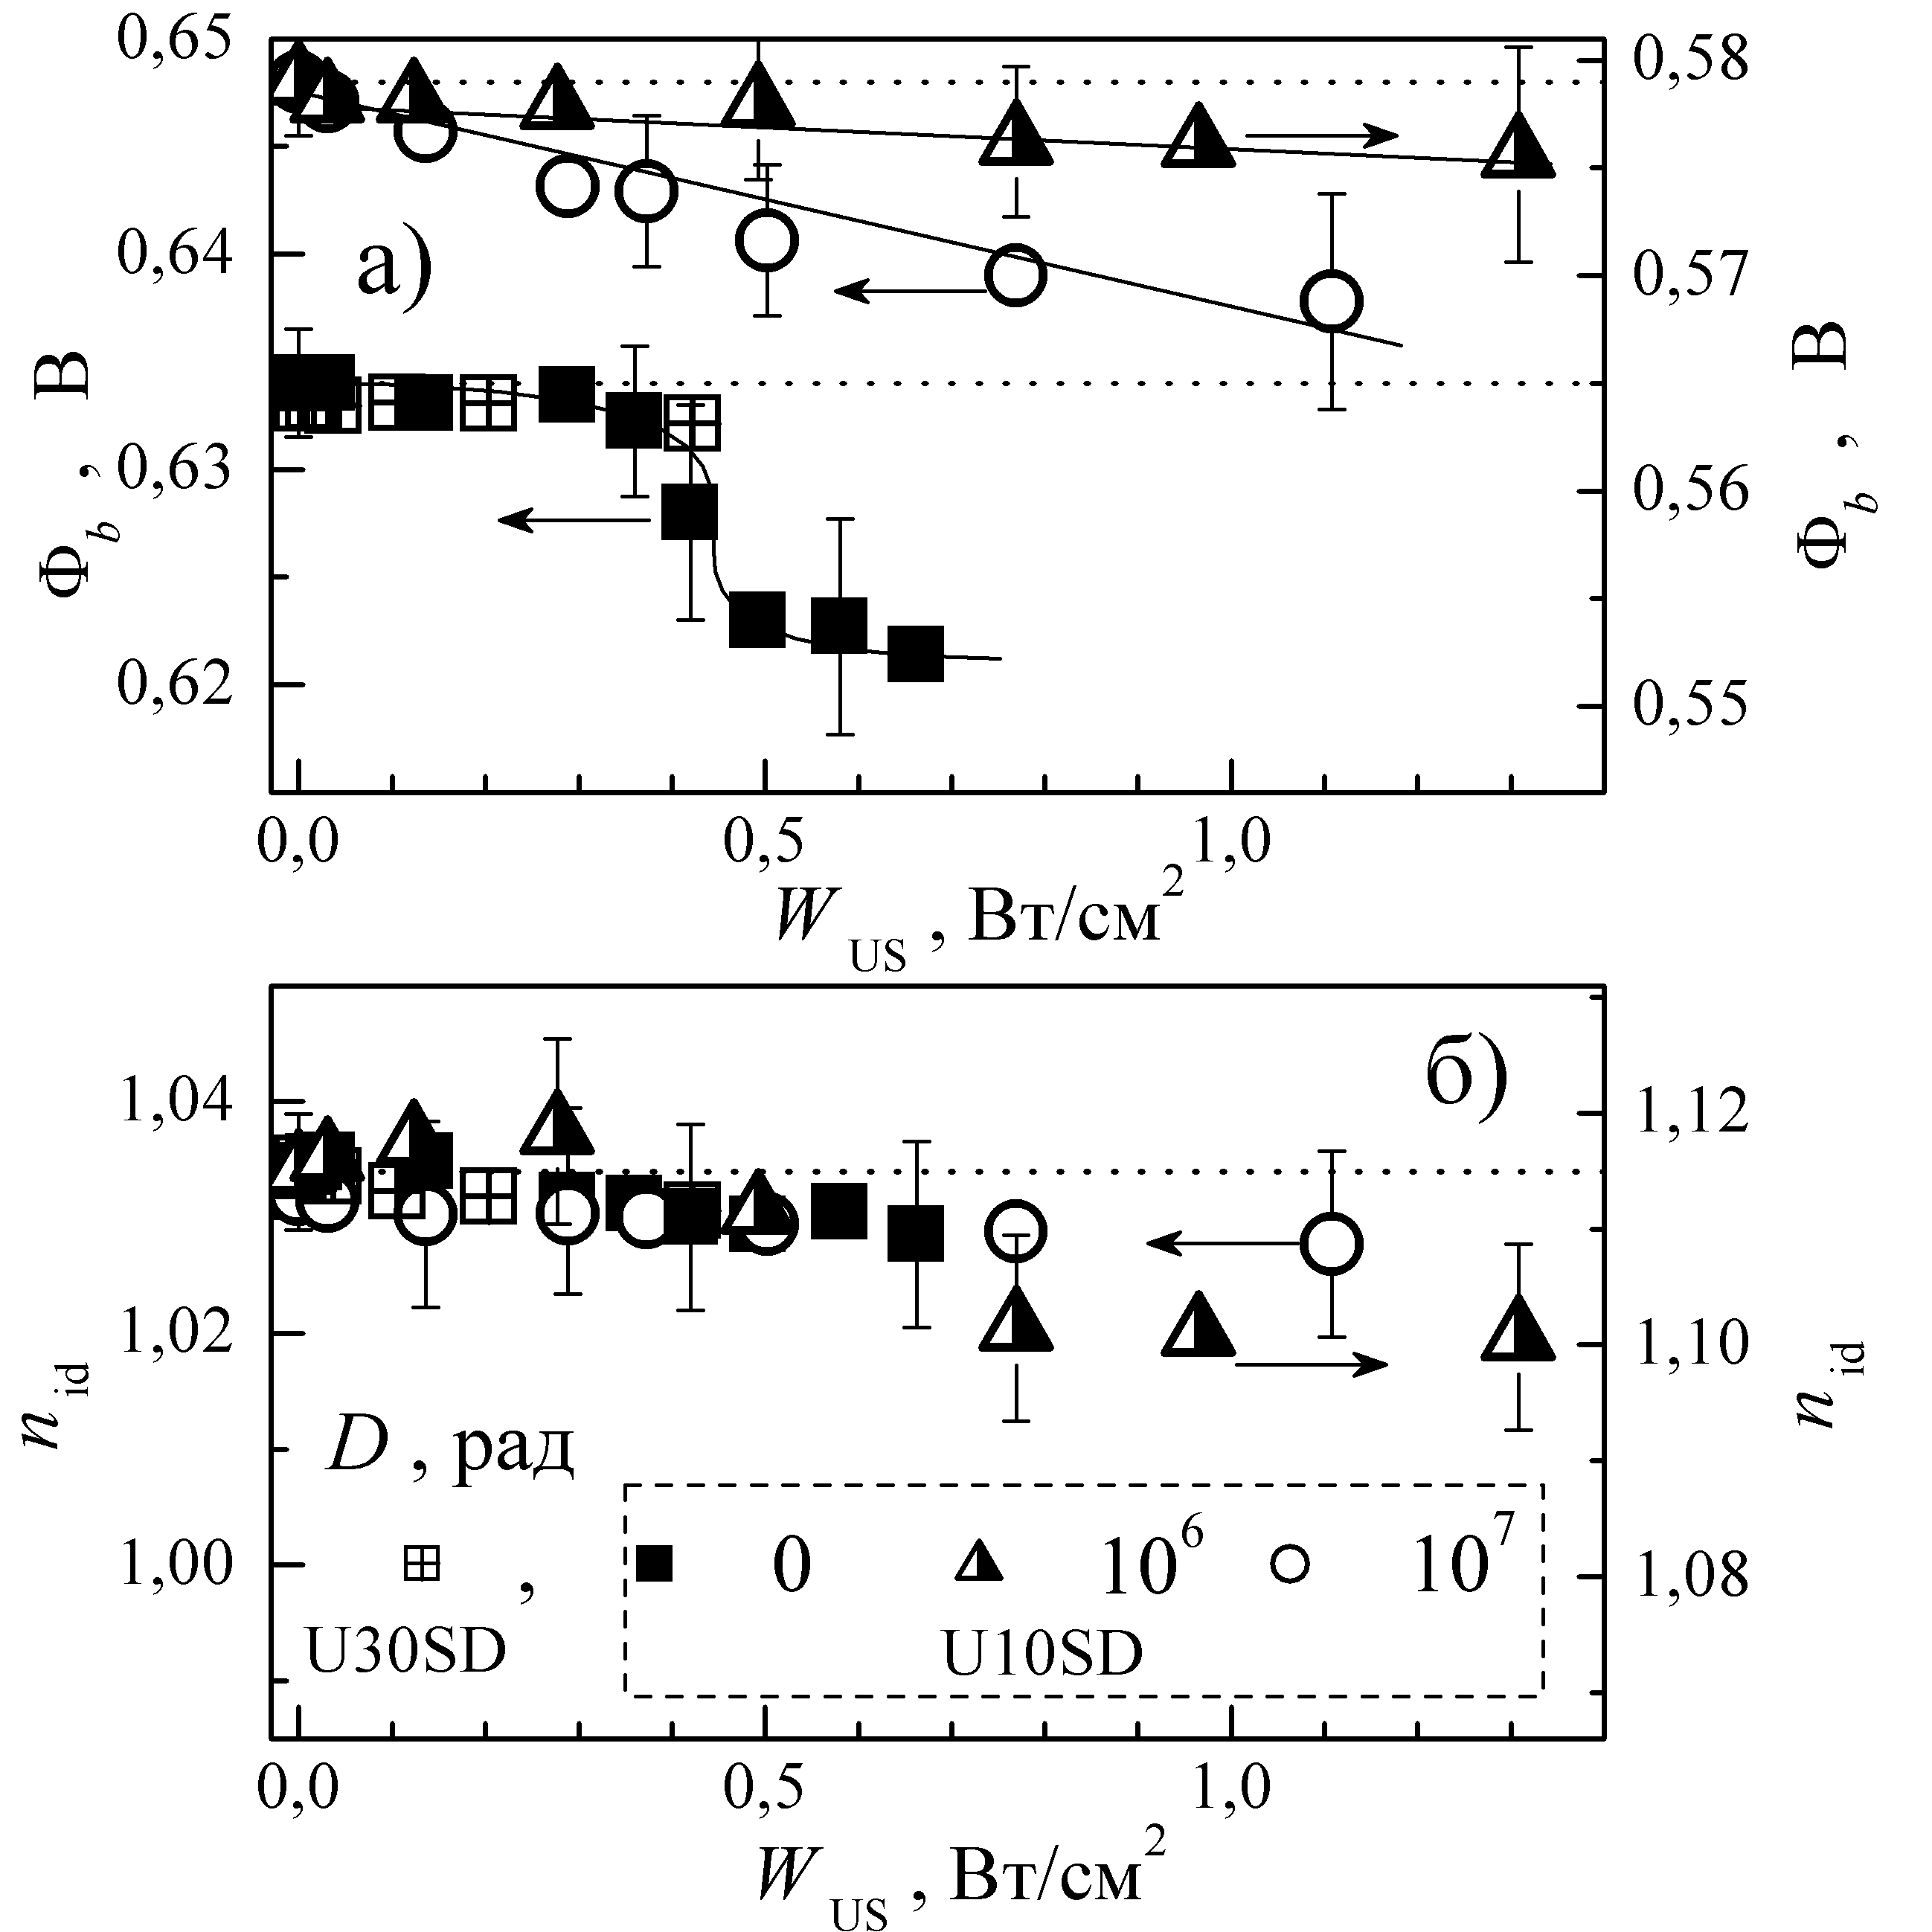
\includegraphics[width=0.6\textwidth]{figFbUSL_SDA}
\caption{\label{figFbUSL_SDA}
Залежності висоти бар'єру Шотткі (а) та фактора неідеальності (б)  від інтенсивності УЗ для
структур Al---$n$--$n^+$--Si з різним ступенем опромінення.
$T=305$~K.
$f_\mathtt{US}=9,6$~МГц.
Горизонтальні пунктирні лінії відповідають значенням параметрів, виміряних без УЗН
}%
\end{figure}

За умов УЗН спостерігається збільшення величини зворотного струму --- рис.~\ref{figIVrg0USL_SDA}.
Ефект послаблюється зі збільшенням зміщення, амплітудна залежність як для неопромінених, так і опромінених структур аналогічна акустоіндукованим змінам висоти бар'єру.
Враховуючи, що акустоіндуковані зміни зворотного струму можуть досягати декількох десятків відсотків,
запропоновано використовувати цей ефект для створення сенсору $\gamma$-–опромінення.
Показано, що акустоіндуковані зміни $I_R$ пов'язані з впливом пружних хвиль лише на ТЕ складову,
тоді як незмінність при УЗН тунельних струму свідчить, що відповідні дефекти (зокрема С$_i$) не є акустоактивними.


У  \underline{\textbf{п'ятому розділі}} представлені результати досліджень
оборотних акустоіндукованих ($f_\mathtt{US}=4,1$, 8,4 та 27,8~МГц) змін параметрів діодів Шотткі Mo---$n$--$n^+$--Si в інтервалі температур $130\div330$~К.
%Зауважимо, що до початку роботи бар'єрні структури на основі малодислокаційних неп'єзоелектричних напівпровідникових кристалів
%залишалися поза увагою науковців з точки зору дослідження низькотемпературних акустоіндукованих ефектів.

\begin{figure}
\center
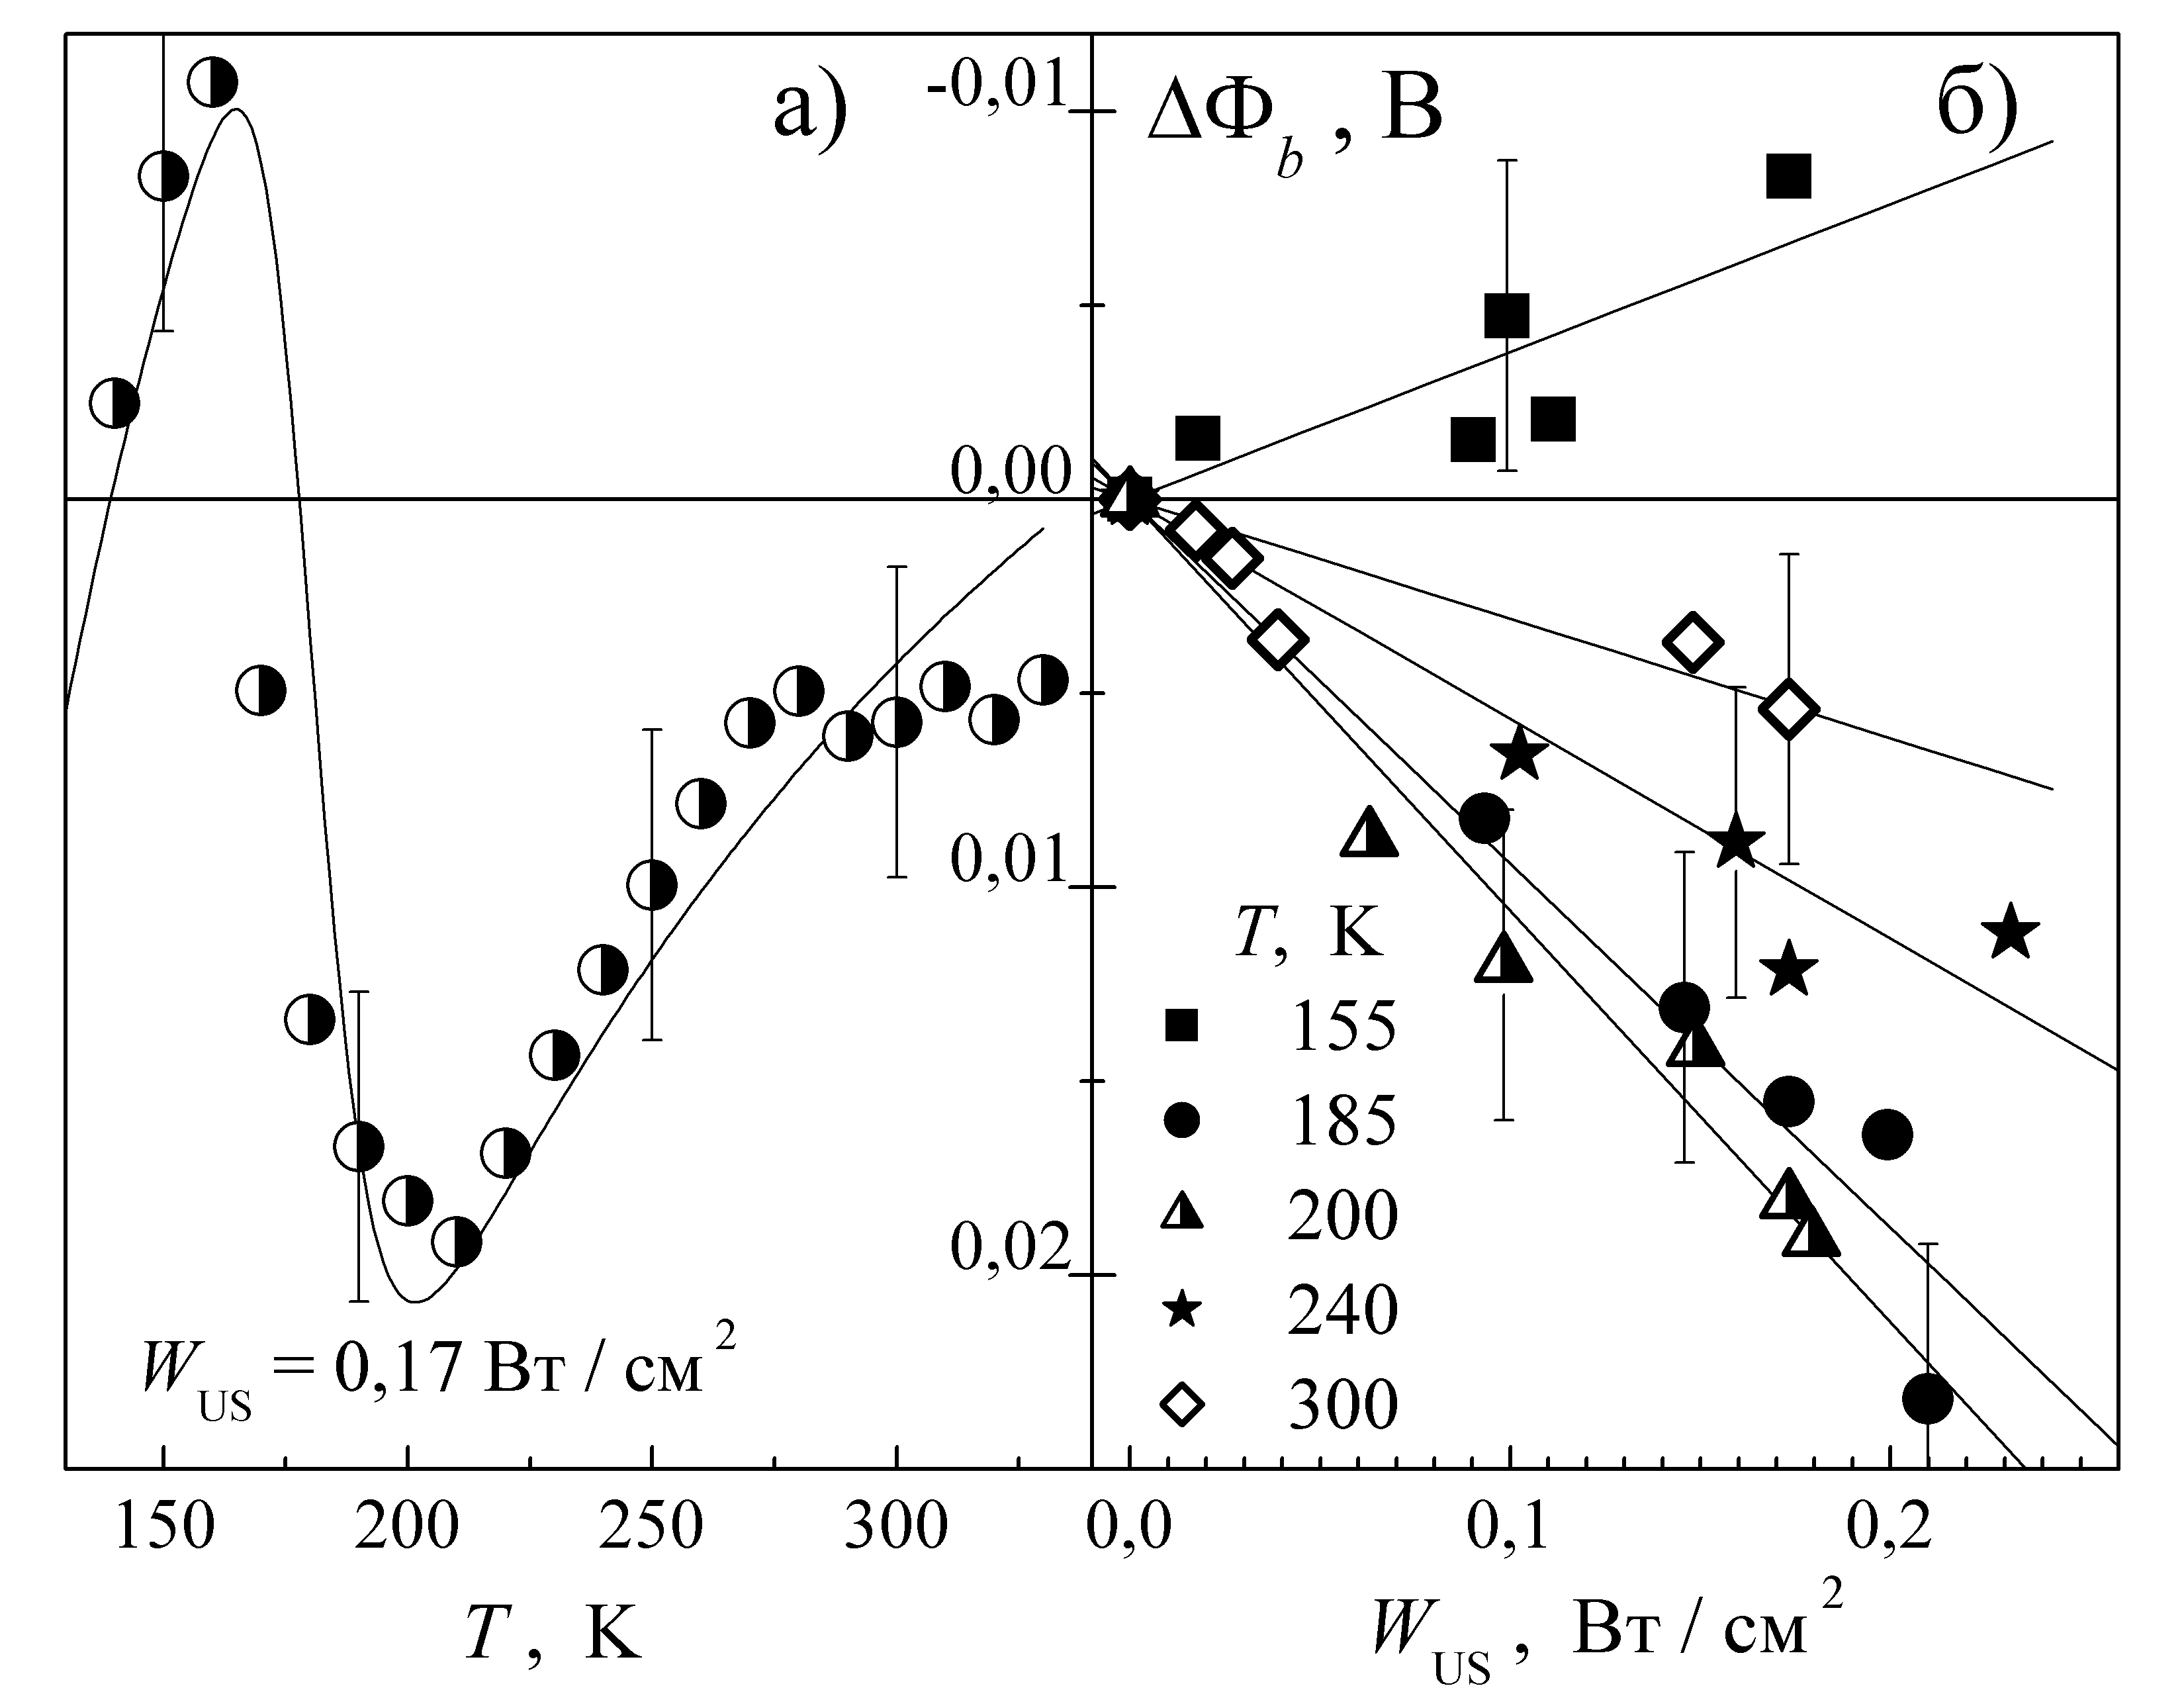
\includegraphics[width=0.6\textwidth]{figDelFbH}
\caption{\label{figDelFbH}
Залежності змін висоти бар'єру високотемпературної компоненти струму від температури (а) та інтенсивності введеного УЗ (б).
$f_\mathtt{US}=4,1$~МГц
}%
\end{figure}

%Апроксимація (метод МАВС) прямих гілок ВАХ проводилася відповідно до виразу
%\begin{equation}
%\label{eqSDB_IV}
%  I=I_{s,H}\left[\exp\left(\frac{qV}{n_\mathrm{id,H}kT}\right)-1\right]+
% I_{s,L}\left\{\exp\left[\frac{q(V-IR_s)}{n_\mathrm{id,L}kT}\right]-1\right\},
%\end{equation}
%тобто струм складається з високотемпературної компоненти (ВТКС, перший доданок), яка при низьких температурах переважала лише при великих зміщеннях та низькотемпературної (НТКС, другий доданок),
%яка спостерігалася лише при $T<220$~К.
Показано, що у досліджених структурах перенесення заряду відбувається відповідно до моделі ТЕ через неоднорідний контакт,
причому для опису температурної залежності висоти бар'єру Шотткі доцільно застосовувати наближення подвійного розподілу Гауса
%\cite{Jiang:DG}
[7$^*$]:
\begin{equation}
\label{eqDG}
  \Phi_{b,H}=-\frac{kT}{q}\ln\left[\varrho_1\exp\left(-\frac{q\Phi_{b,1}^0}{kT}+
  \frac{q^2\sigma^2_{\Phi,1}}{2k^2T^2}\right)
   +
  \varrho_2\exp\left(-\frac{q\Phi_{b,2}^{0}}{kT}+
  \frac{q^2\sigma^2_{\Phi,2}}{2k^2T^2}\right)\right],
\end{equation}
$\varrho_1$, $\varrho_2$  --- вагові коефіцієнти кожного з розподілів.
Виявлено, що ультразвук викликає оборотні збільшення фактора неідеальності та зміни $\Phi_{b}$,
величина і знак яких залежить від температури --- рис.~\ref{figDelFbH}.
Розрахунки, проведені відповідно до моделі
%\cite{Tung:MSE,Jiang:DG}
[3$^*$,7$^*$] показали, що за умов УЗН відбувається зростання
$\Phi_{b,1}^0$ (від 780~мВ до, наприклад при $f_\mathtt{US}=4,1$~МГц, $W_\mathtt{US}=0,17$~Вт/см$^2$,  810~мВ),
$\Phi_{b,2}^0$ (від 1100 до  1200~мВ),
$\sigma_{\Phi,1}$ (від 20 до  50~мВ),
$\sigma_{\Phi,2}$ (від 120 до  130~мВ) та
зростання внеску другого розподілу (в чотири рази).
Також виявлено,
%Аналіз НТКС показав,
що УЗН викликає зміни висоти бар'єру в області патчів, які немонотонним чином залежать від $W_\mathtt{US}$;
зростання ефективної густини патчів (від від 0,2 до 2~мм$^{-2}$) та зменшення (від $2,7\cdot10^{-5}$ до $2,5\cdot10^{-5}$ м$^{2/3}\cdot$В$^{1/3}$)
величини $3(R_p^2\Delta_p/4)^{1/3}$, де $\Delta_p$ та $R_p$ --- зниження висоти бар'єру в області патча та його розмір, відповідно.
Основні виявлені особливості впливу УЗН на стан контакту метал--напівпровідник якісно узагальнено на рис.\ref{figBand}.



\begin{figure}
\center
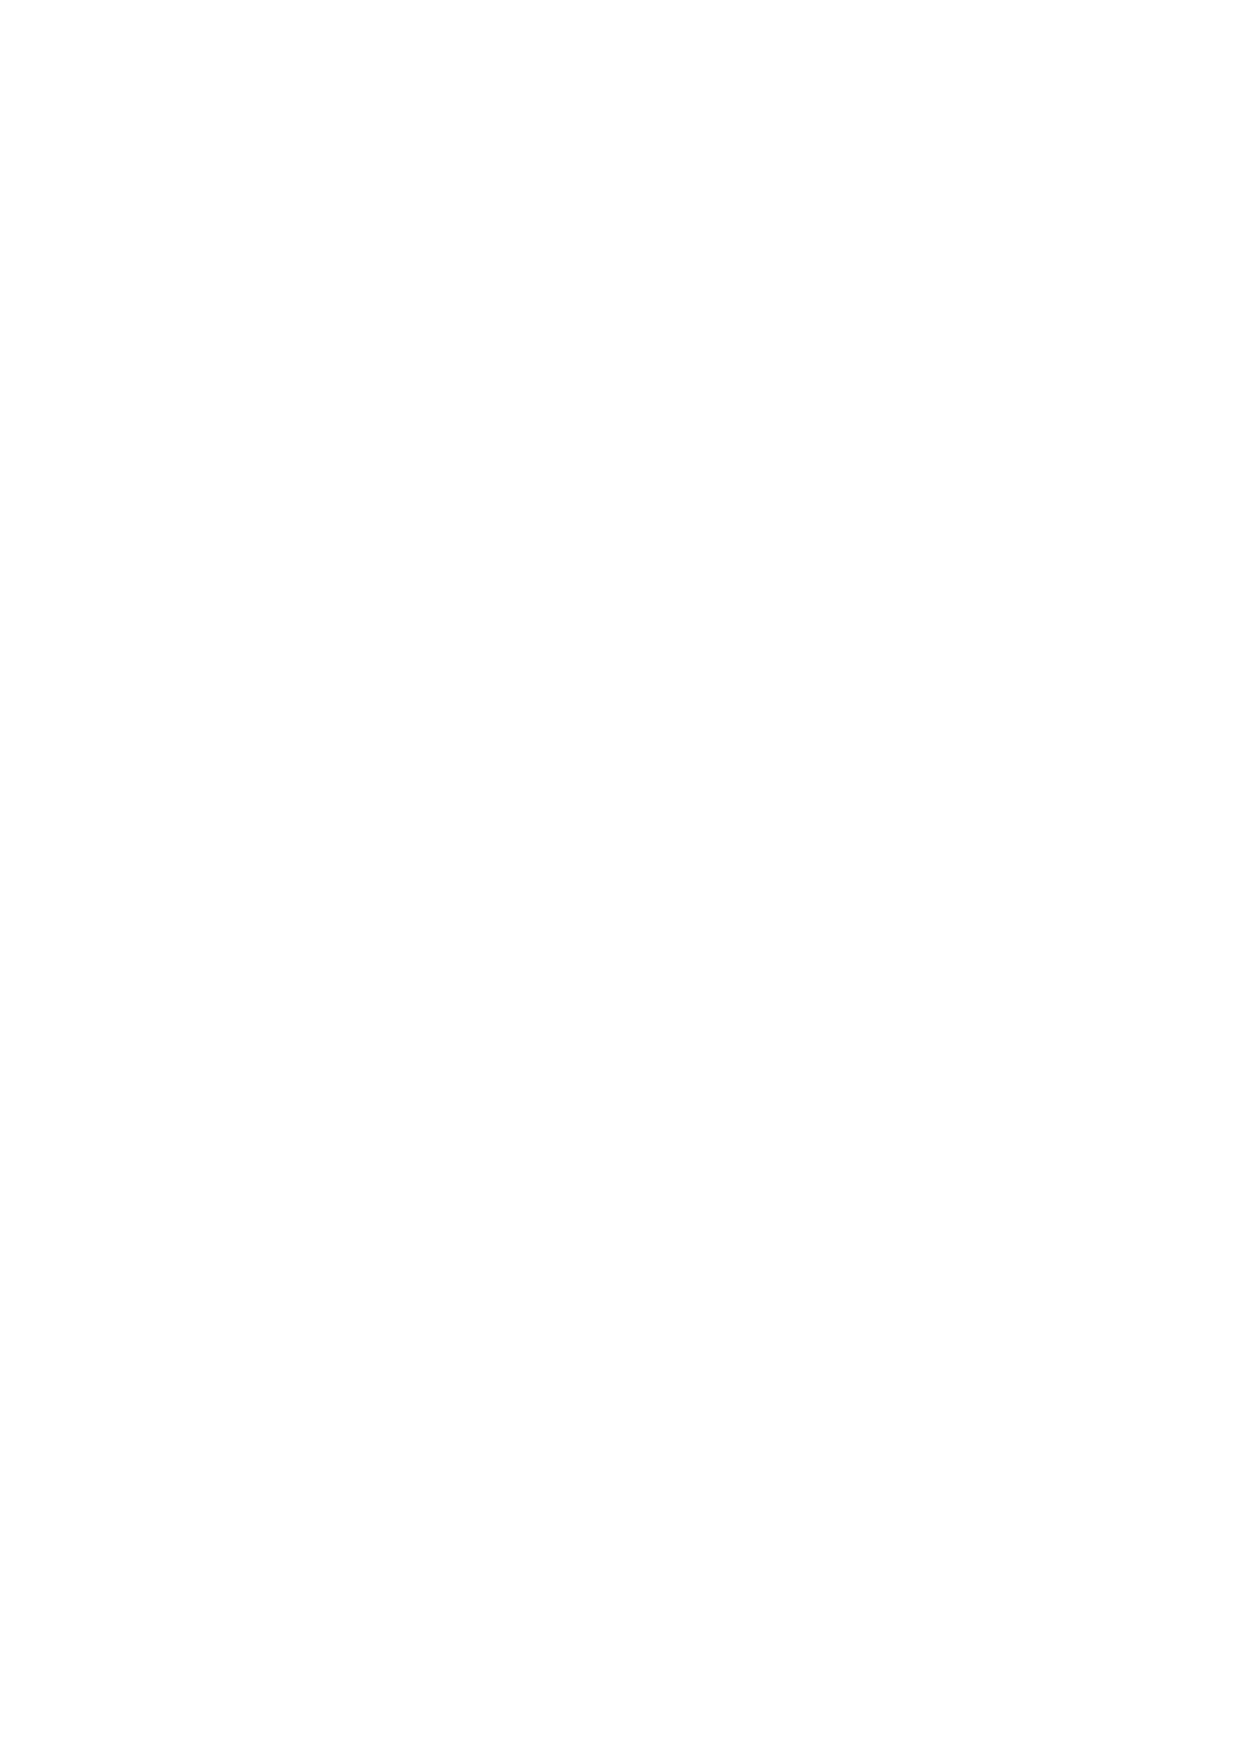
\includegraphics[width=0.55\textwidth]{figBand}
\caption{\label{figBand}
Схематичне зображення
просторового розподілу поверхневого потенціалу
%зони провідності,
що відображає різницю між випадком УЗН (верхня площина та верхня контурна поверхня) та
його відсутністю (нижня площина та нижня контурна поверхня).
Рисунок зроблено у припущенні, що наявні два патчі.
%При розрахунку потенціальних поверхонь була використана формула~(1.5.3) з
%\cite{Tung:MSE}
%[5$^*$]
\vspace{1em}
}%
\end{figure}

\begin{figure}[b]
\center
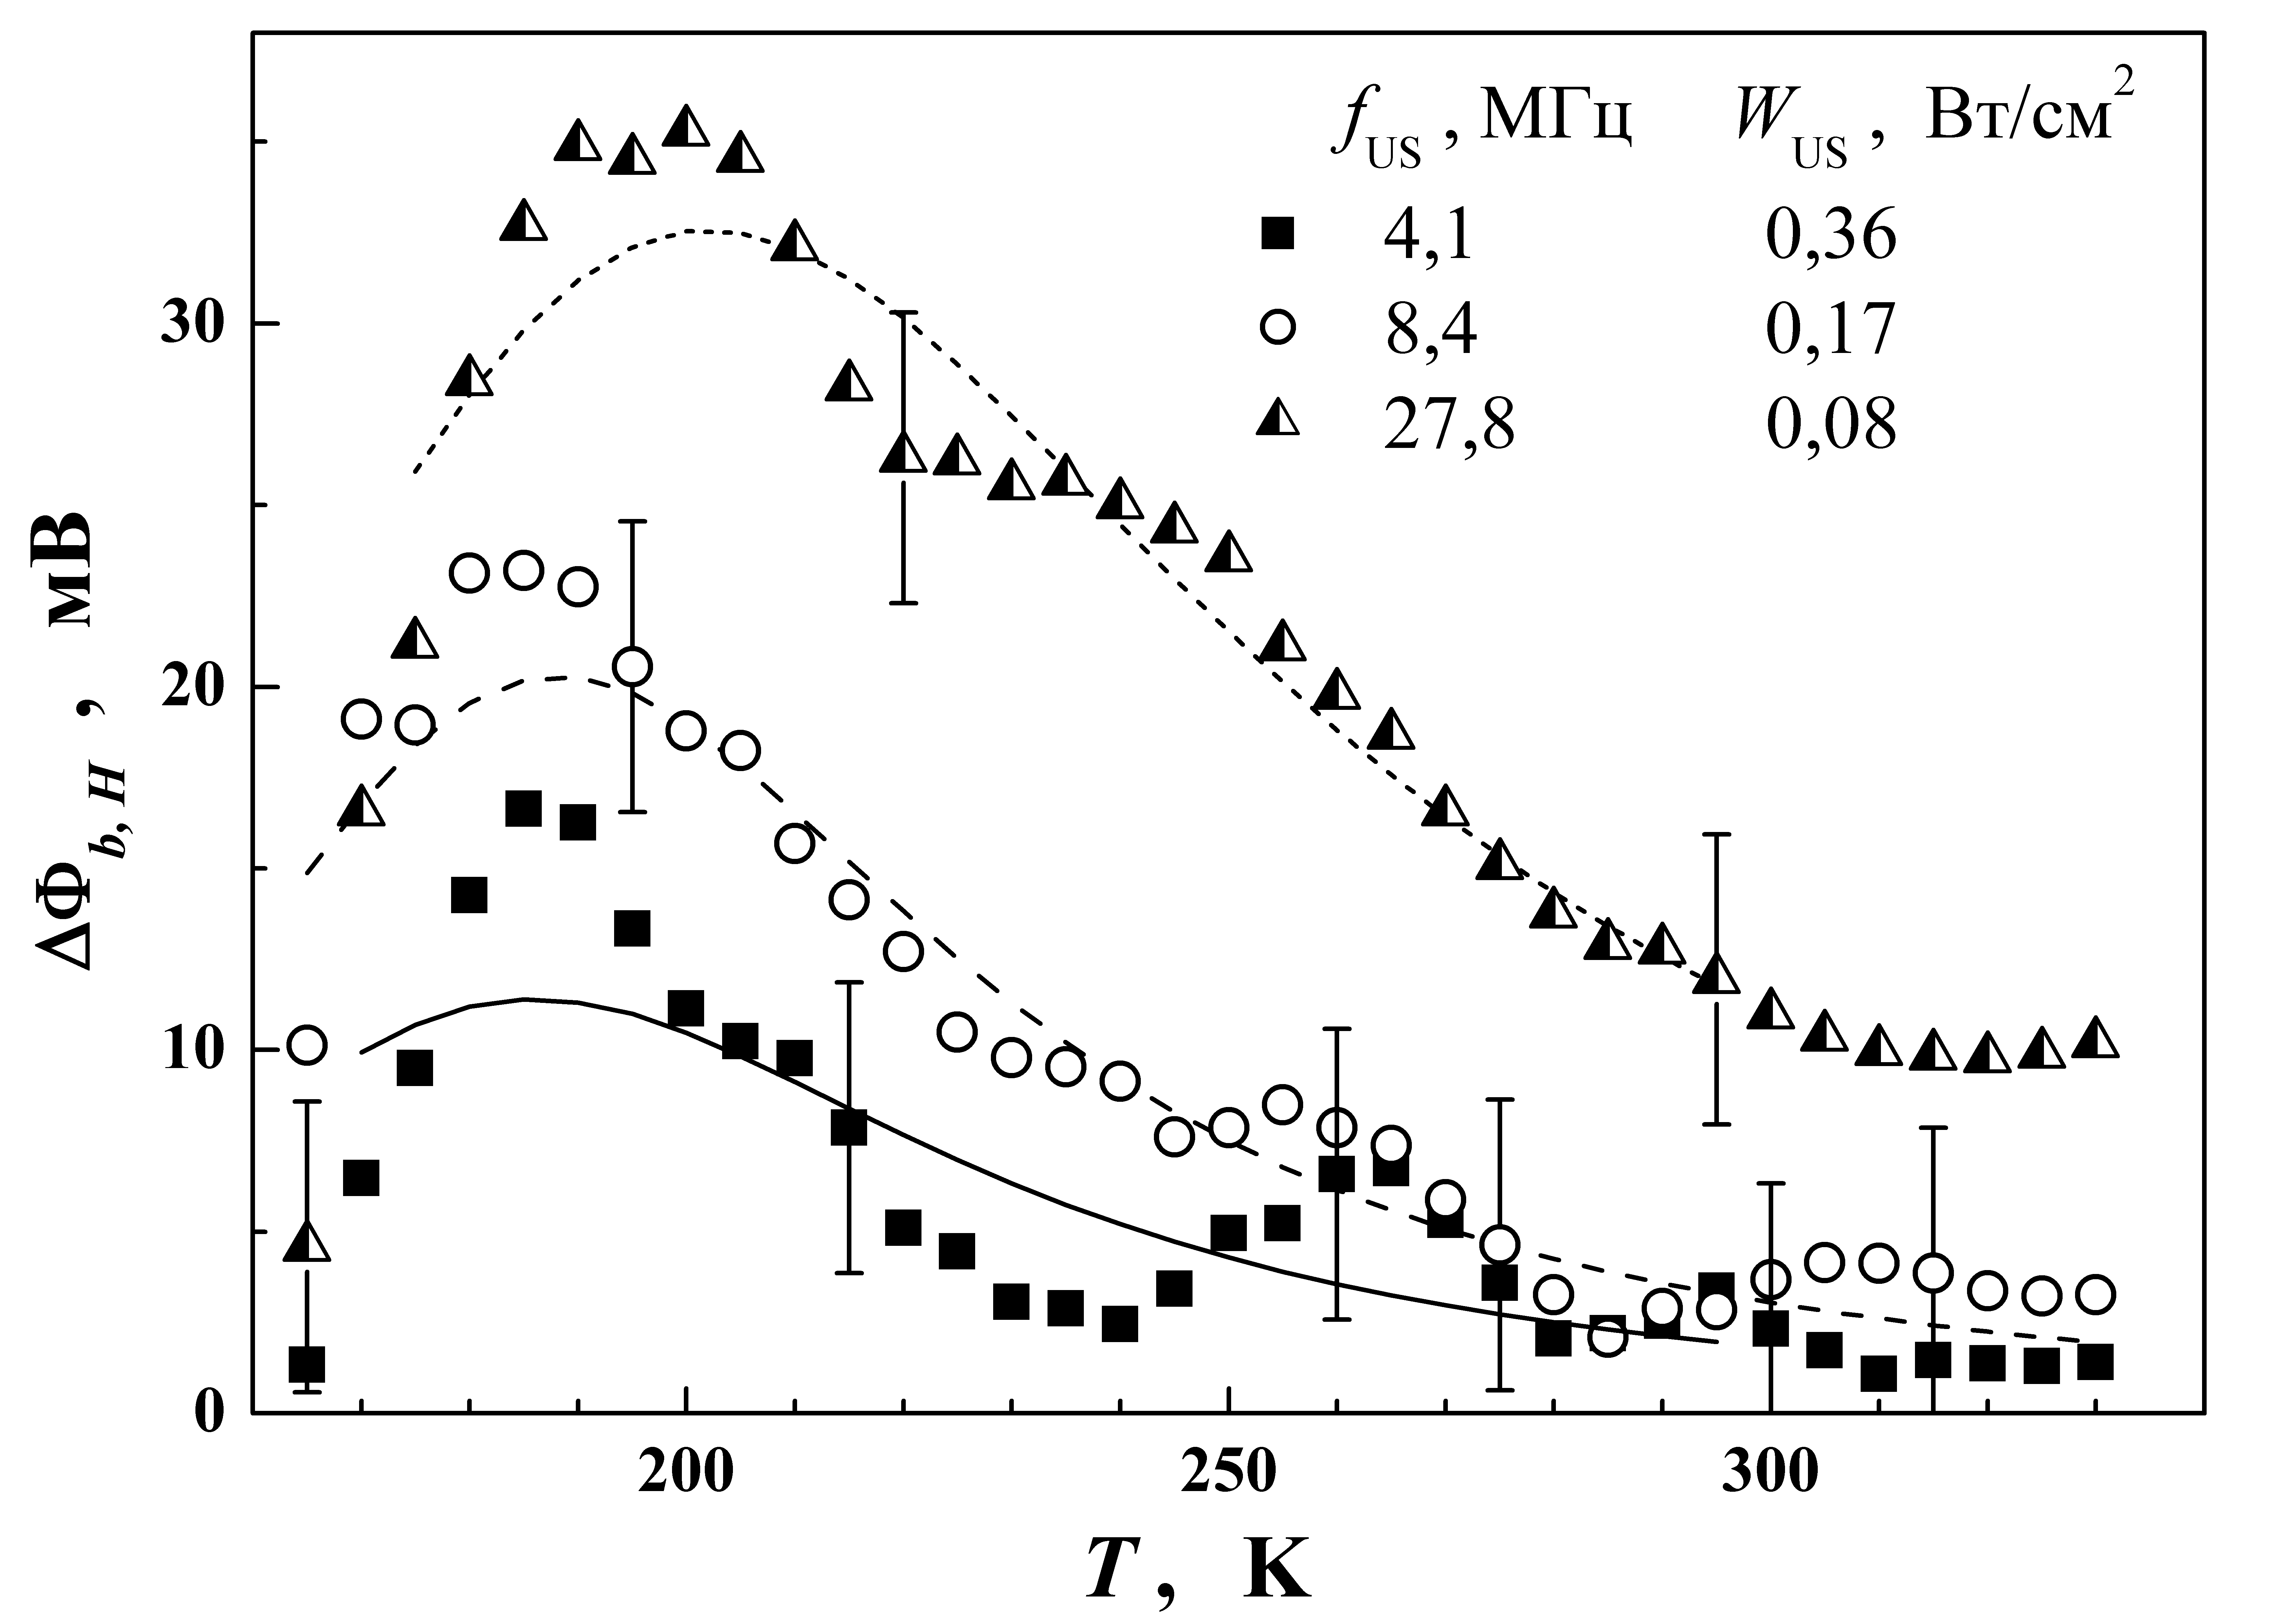
\includegraphics[width=0.6\textwidth]{figDelFbT_SDB}
\caption{\label{figDelFbT_SDB}
Температурні залежності змін висоти бар'єру Шотткі при УЗН на різних частотах.
Точки --- експеримент,
лінії --- апроксимація згідно з формулою~(\ref{eqBr})
}%
\end{figure}
Встановлено, що температурні та частотні залежності акустоіндукованих змін в структурах
 Mo---$n$--$n^+$--Si (рис.\ref{figDelFbT_SDB}) можуть бути пояснені в рамках моделі Брейсфолда
% \cite{Brailsford}
[8$^*$],
яка передбачає акстостимульовану дифузію дислокаційних перегинів.
Зокрема, зміни висоти бар'єру описуються виразом
\begin{equation}
\label{eqBr}
\Delta\Phi_{b,H}\,(f_\mathtt{US},\,T)\sim\frac{f_\mathtt{US}}{T}\frac{(f_\mathtt{US}/{f_k})\exp\left(\frac{W_k}{kT}\right)}
{1+(f_\mathtt{US}/{f_k})^2\exp\left(\frac{2W_k}{kT}\right)}W_\mathtt{US},
\end{equation}
де
$W_k$ --- енергія активації дифузії,
а параметр $f_k$ пов'язаний з середньою довжиною дислокаційного сегмента та абсолютним значенням коефіцієнта дифузії.
%В досліджених структурах ці дефекти пов'язані з патчами,
Визначені в рамках моделі величини становлять $W_k=(90\pm10)$~меВ та $f_k=(3\pm2)\cdot10^9$~Гц.


Виявлено, що при зворотному зміщенні
%Дослідження зворотного струму показали, що
а)~перенесення заряду пов'язане з процесами ТЕ ($I_{TE}$) та тунелюванням, стимулюваним фононами, з електронних станів поблизу границі розділу ($I_{P\!AT}$)
%\cite{Pipinys2006}
[9$^*$]
і може бути описане виразом
\begin{eqnarray}
\label{eqIgen}
 I_R&=&I_{TE}+I_{P\!AT}=P_tI_0\,T^2\exp\left(-\frac{q\Phi_b}{kT}\right)\left[1-\exp\left(-\frac{V_s}{kT}\right)\right]+\\
 &&+\frac{P_tq^2F_mAN_{ss}}{\sqrt{8m^*\epsilon_t}}\left(1-\frac{\gamma}{\gamma_1}\right)^{1/2}\exp
    \left\{-\frac{4\sqrt{2m^*}\,\epsilon_t^{3/2}\left(\gamma_1-\gamma\right)^2}{3qF_m\hbar} \nonumber
    [\gamma_1+\frac{1}{2}\gamma]\right\}\\ \nonumber
%        P_t&=&\exp\left\{-\frac{4\sqrt{2m_i^*q}}{3\hbar V_i}\left[(U_0+V_i)^{\,3/2}-U_0^{\,3/2}\right]\delta\right\}\,,\\ \nonumber
    \gamma_1&=&(1+\gamma^2)^{1/2}, \quad
    %\\ \nonumber
    \gamma=\frac{a_\mathtt{e-ph}\hbar\omega_{ph}^2\sqrt{2m^*}}{qF_m\sqrt{\epsilon_t}}
    \left\{\frac{\exp\left(\frac{\hbar\omega_{ph}}{kT}\right)+1}{\exp\left(\frac{\hbar\omega_{ph}}{kT}\right)-1}\right\},   \nonumber
\end{eqnarray}
де
$P_t$ --- ймовірність тунелювання через діелектричний прошарок,
$N_{ss}$ --- густина заповнених рівнів поблизу інтерфейсу,
$\hbar\omega_{ph}$ --- енергія фонону,
$a_\mathtt{e-ph}$ --- константа електрон--фононної взаємодії,
$\epsilon_t$ --- глибина залягання рівнів,
$F_m$ --- напруженість електричного поля на границі напівпровідник--метал;
б)~висота бар'єру та $\epsilon_t$ зменшуються при зростанні зворотної напруги
($\Phi_{b}=\Phi_{b0}-\alpha_{F} F_m$,
$\epsilon_t=\epsilon_{t0}-\beta_F F_m^{1/2}$), що пов'язано з впливом інтерфейсних станів
%\cite{Tung:MSE}
[5$^*$] та ефектом Пула--Френкеля;
в)~за умов УЗН зареєстроване оборотне зростання $I_R$, викликане акустоіндукованим зменшенням ряду параметрів --- див. табл.~\ref{tabSDBParZv};
г)~причиною появи тунелювання є кластери позитивно заряджених дефектів, а акустоіндукованих змін $I_{P\!AT}$ --- модифікація розміру кластера, викликана
локальним підвищенням температури скупчення дефектів у акустичному полі
%\cite{MirzadeJAP2011}
[2$^*$].

%\begin{figure}
%\center
%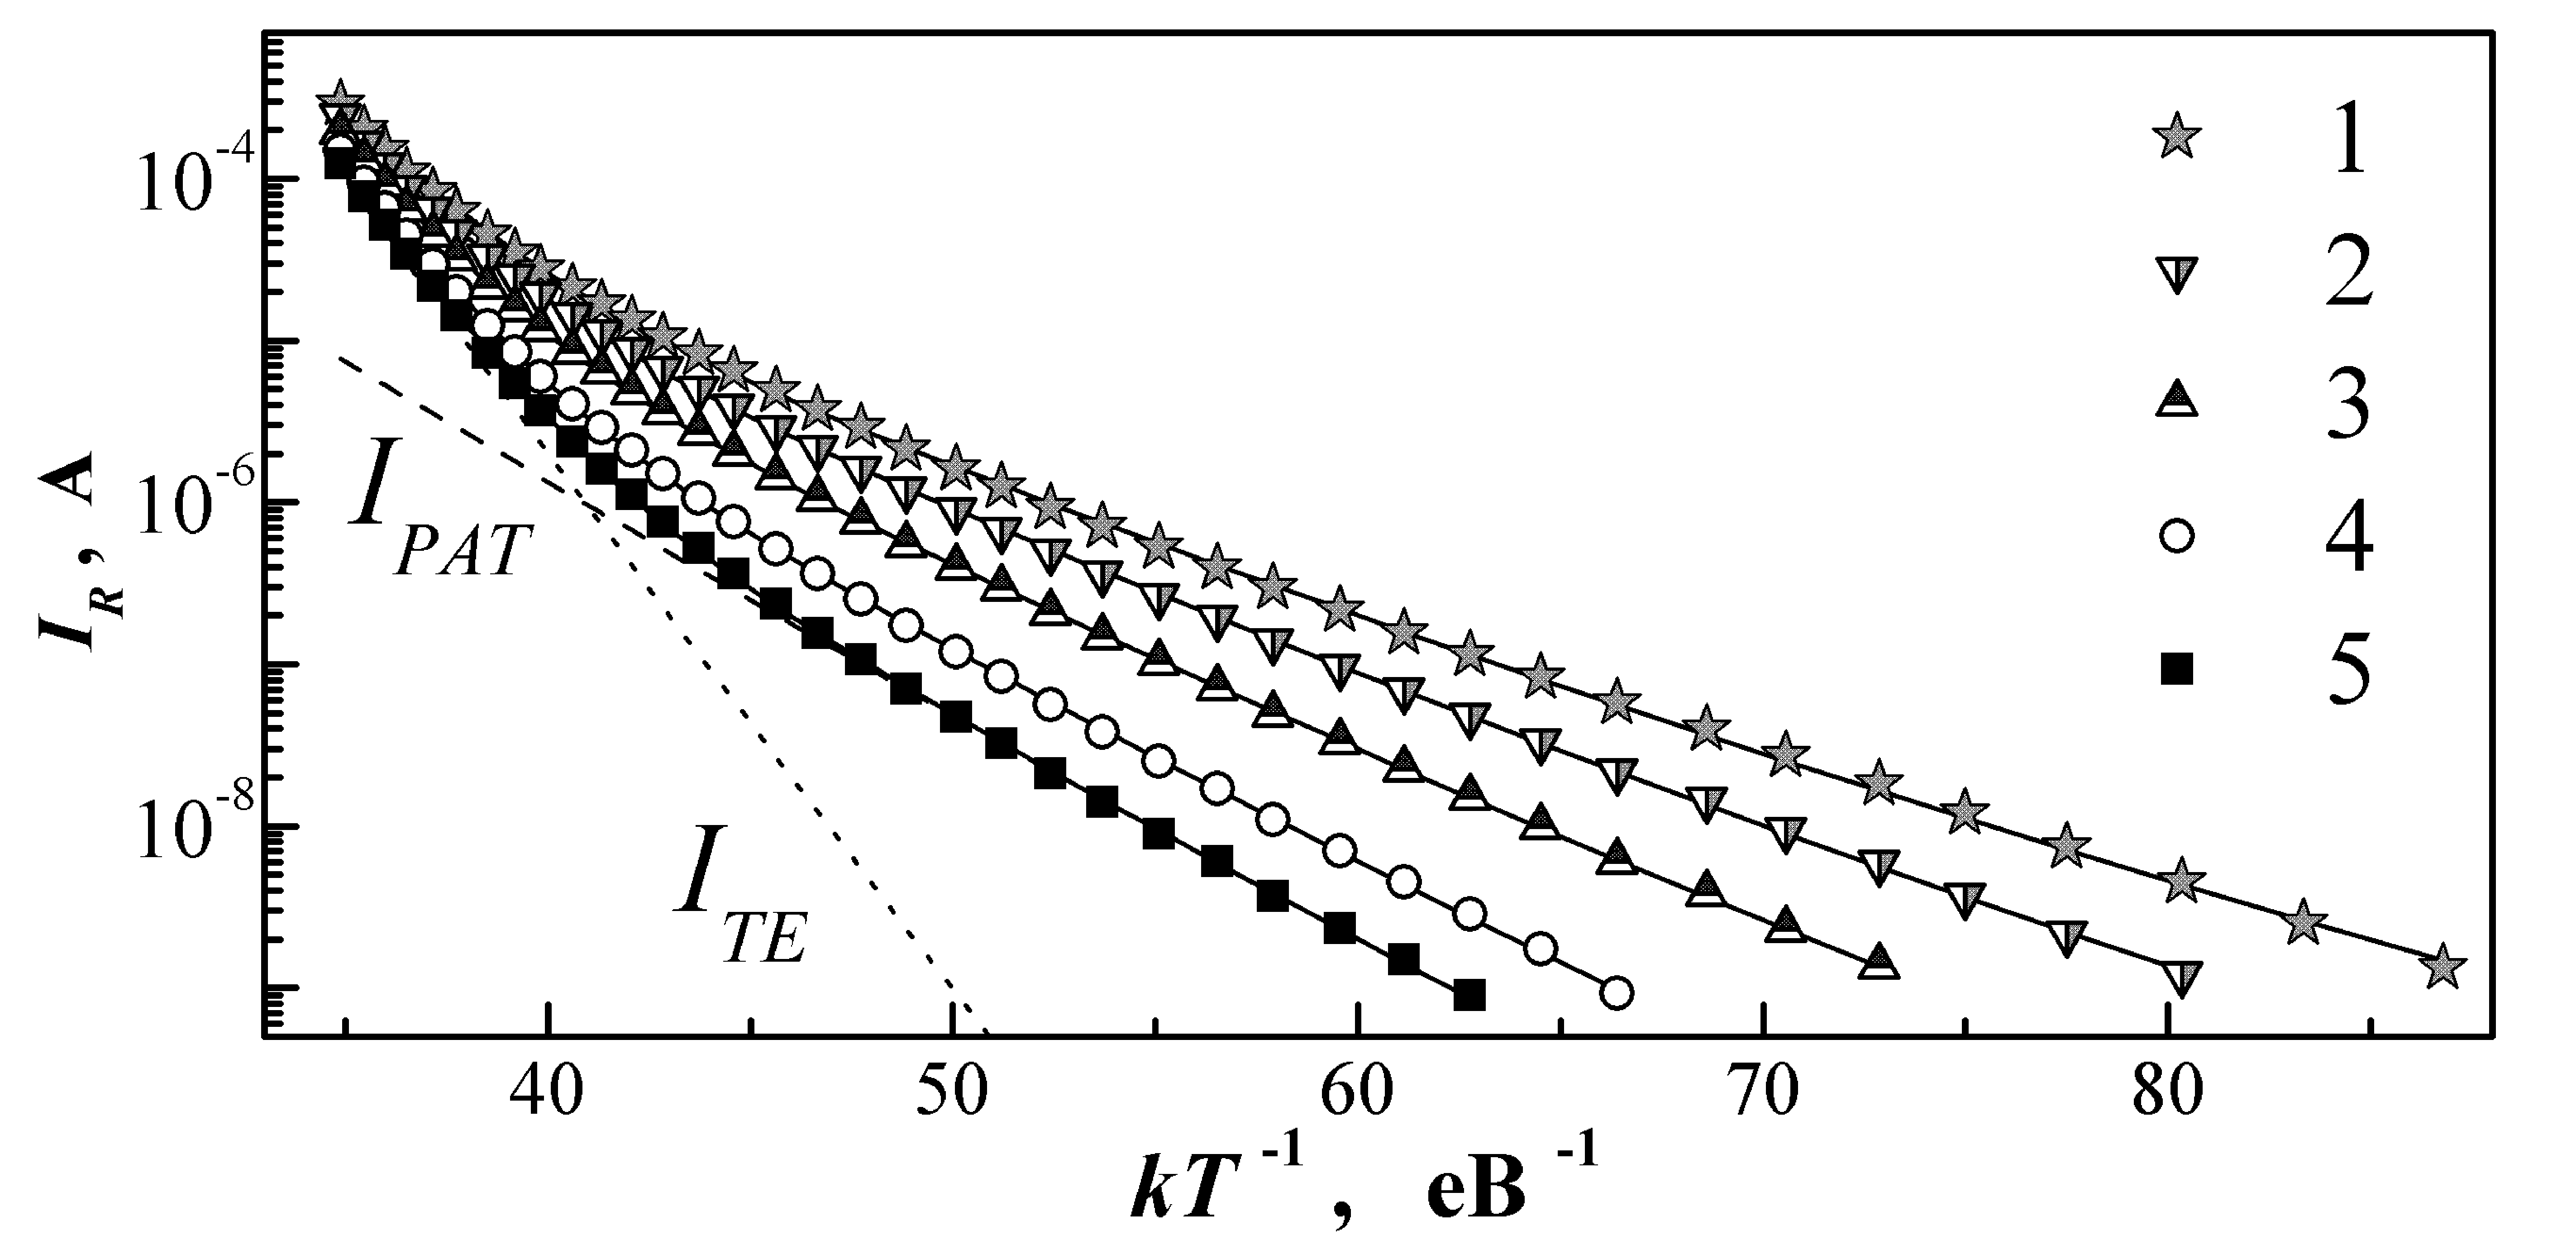
\includegraphics[width=0.7\textwidth]{figKT_SDB}
%\caption{\label{figKT_SDB}
%Залежності зворотного струму структур Mo$/n-n^+$--Si від оберненої температури,
%виміряні при різних напругах зміщення.
%Точки --- експеримент,
%суцільні лінії --- апроксимація відповідно до формули~(\ref{eqIgen}).
%Пунктирна та штрихована лінії відображають ТЕ та РАТ компоненти струму, відповідно
%}%
%\end{figure}


\begin{table}[hb]
\caption{Параметри, визначені для структур Mo---$n$--$n^+$--Si зі зворотних гілок ВАХ за умов УЗН та без нього}
\label{tabSDBParZv}
\centering
\begin{tabular}{|c|c|c|c|c|c|c|}
\hline
$W_\mathtt{US}$, &$f_\mathtt{US}$,&$\Phi_{b0}(0)$,&$\alpha_F$,&$\epsilon_{t0}$,&$\beta_F\cdot10^{5}$,&$N_{ss}$,\\
Вт/см$^2$&МГц&мВ&нм&меВ&еВ$\cdot$м$^{1/2}\cdot$В$^{-1/2}$&$10^{11}$см$^{-2}$\\\hline
0&---&$960\pm10$&$66\pm7$&$610\pm10$&$10,5\pm0,3$&$5,3\pm0,7$\\\hline
0,17&8,4&$870\pm10$&$51\pm5$&$540\pm10$&$\;\:8,1\pm0,5$&$1,2\pm0,2$\\\hline
0,65&4,1&$790\pm10$&$36\pm7$&$520\pm10$&$\;\:7,1\pm0,5$&$0,8\pm0,2$\\\hline
\end{tabular}
\end{table}

У  \underline{\textbf{шостому розділі}} представлені результати досліджень необоротних змін арсенід галієвих структур, викликаних мікрохвильовою та ультразвуковою обробками.

Зокрема, досліджено вплив надвисокочастотного випромінювання (частота 2,45 ГГц, питома потужність  $1,5$~Вт/см$^2$, час обробки --- до 80~c) на параметри глибоких центрів, розташованих у приповерхневій області монокристалів $n$--6$H$--SiC та $n$--GaAs, а також арсенід галієвих епітаксійних структур за допомогою методу акустоелектричної релаксаційної спектроскопії.
Виявлено, що до опромінення в структурах спостерігаються комплекси вакансійного типу:
%
%Шляхом порівняння отриманих величин енергетичного положення рівнів з літературними даними проведено ідентифікацію відповідних дефектів у приповерхневому шарі монокристалів та на границі розділу епітаксійних структур.
%Зокрема до опромінення виявлені комплекси вакансійного типу:
V$_\text{Si}$V$_\text{C}$ (положення рівня $E_c-0,33$~еВ) в $n$--6$H$--SiC
та V$_\text{As}$ ($E_c-0,32$~еВ) і V$_\text{Ga}$Ga$_i$V$_\text{As}$ ($E_c-0,49$~еВ) в $n$--GaAs,
а також V$_\text{Ga}$V$_\text{As}$ ($E_c-0,24$~еВ), V$_\text{As}$As$_i$ ($E_c-(0,43-0,46)$~еВ) і
 V$_\text{Ga}$Ga$_\text{As}$ ($E_c-0,40$~еВ) на границі розділу епітаксійних структур $n$--$n^+$--GaAs.
Внаслідок мікрохвильового опромінення біля поверхні збільшується концентрація міжвузольних атомів та відбуваються перетворення в дефектній
підсистемі внаслідок їх взаємодії з вихідними дефектами:
\begin{eqnarray*}
  \text{SiC}&:&\text{V}_\text{Si}\;\text{V}_\text{C}+\text{V}_\text{Si}\;\text{V}_\text{C}+\text{C}_{\,i}+ \text{C}_{\,i} \rightarrow \text{V}_\text{Si}+ \text{V}_\text{Si}\rightarrow \text{V}_\text{Si}\;\text{V}_\text{Si}\,;\\
  &&\text{V}_\text{Si}\;\text{V}_\text{Si}+\text{Si}_{\,i}+ \text{Si}_{\,i} \rightarrow 0\,;\\
  \text{GaAs}&:&\text{V}_\text{As}+ \text{As}_{\,i} \rightarrow\text{V}_\text{Si}\;\text{As}_{\,i} \rightarrow 0\,;\\
   &&  \text{V}_\text{Ga}\;\text{Ga}_{\,i}\;\text{V}_\text{As}\rightarrow \text{Ga}_\text{Ga}\;\text{V}_\text{As}
  \rightarrow \text{Ga}_\text{As}\;\text{V}_\text{Ga} \,;\\
  &&\text{V}_\text{Ga}\;\text{V}_\text{As}+\text{Ga}_{\,i}+\text{As}_{\,i} \rightarrow \text{V}_\text{As}\;\text{As}_{\,i}\,;\\
  &&  \text{V}_\text{Ga}\;\text{Ga}_\text{As}+\text{As}_{\,i} \rightarrow
  \text{Ga}_\text{Ga}\;\text{V}_\text{As}+\text{As}_{\,i} \rightarrow
  \text{V}_\text{As}\;\text{As}_{\,i}\,.
\end{eqnarray*}
Крім того, мікрохвильова обробка викликає модифікацію (у декілька разів) поперечного перерізу захоплення електронів,
яка пов'язані зі зміною напруженості електричного поля в околі дефектів.
Отримані результати щодо зміни параметрів дефектів корелюють з вимірами радіуса кривизни структур та деформації у приповерхневому шарі.
Показано, що наявність механічних напруг сприяє радіаційно стимульованим перетворенням точкових дефектів.


Також досліджено вплив ультразвукової обробки
($f_\mathtt{US}=(4,1\div30)$~МГц, $W_\mathtt{US}=(0,3\div3)$~Вт/м$^2$, час обробки $t_\mathtt{UST}=(5\div15)$~год) на параметри структур
Au--TiB$_x$--$n$--$n^+$--GaAs, виготовлених
за технологією з інтегральним тепловідведенням.
Виявлено, що при $W_\mathtt{US}<2,5$~Вт/м$^2$ УЗО викликає зменшення розкиду висоти бар'єру, фактора неідеальності та величини зворотного струму (рис.~\ref{figIrG_GA})
діодів Шотткі, виготовлених в єдиному технологічному процесі.
Ефект пов'язаний акустостимульованою дифузією точкових дефектів, яка призводить до згладжування локальних неоднорідностей границі розділу.
Виявлено, що зі збільшенням частоти ультразвука інтенсифікуються процеси перебудови дефектів, що відображається у зміні характеристичного  параметра тунельної компоненти зворотного
струму.
При перевищенні $W_\mathtt{US}$ порогу ($\sim2,5$~Вт/см$^2$) спостерігається зменшення $\Phi_b$ та зростання $n_\mathrm{id}$ і зворотного струму, що пов'язано з генерацією дефектів акустичною хвилею.

\begin{figure}
\center
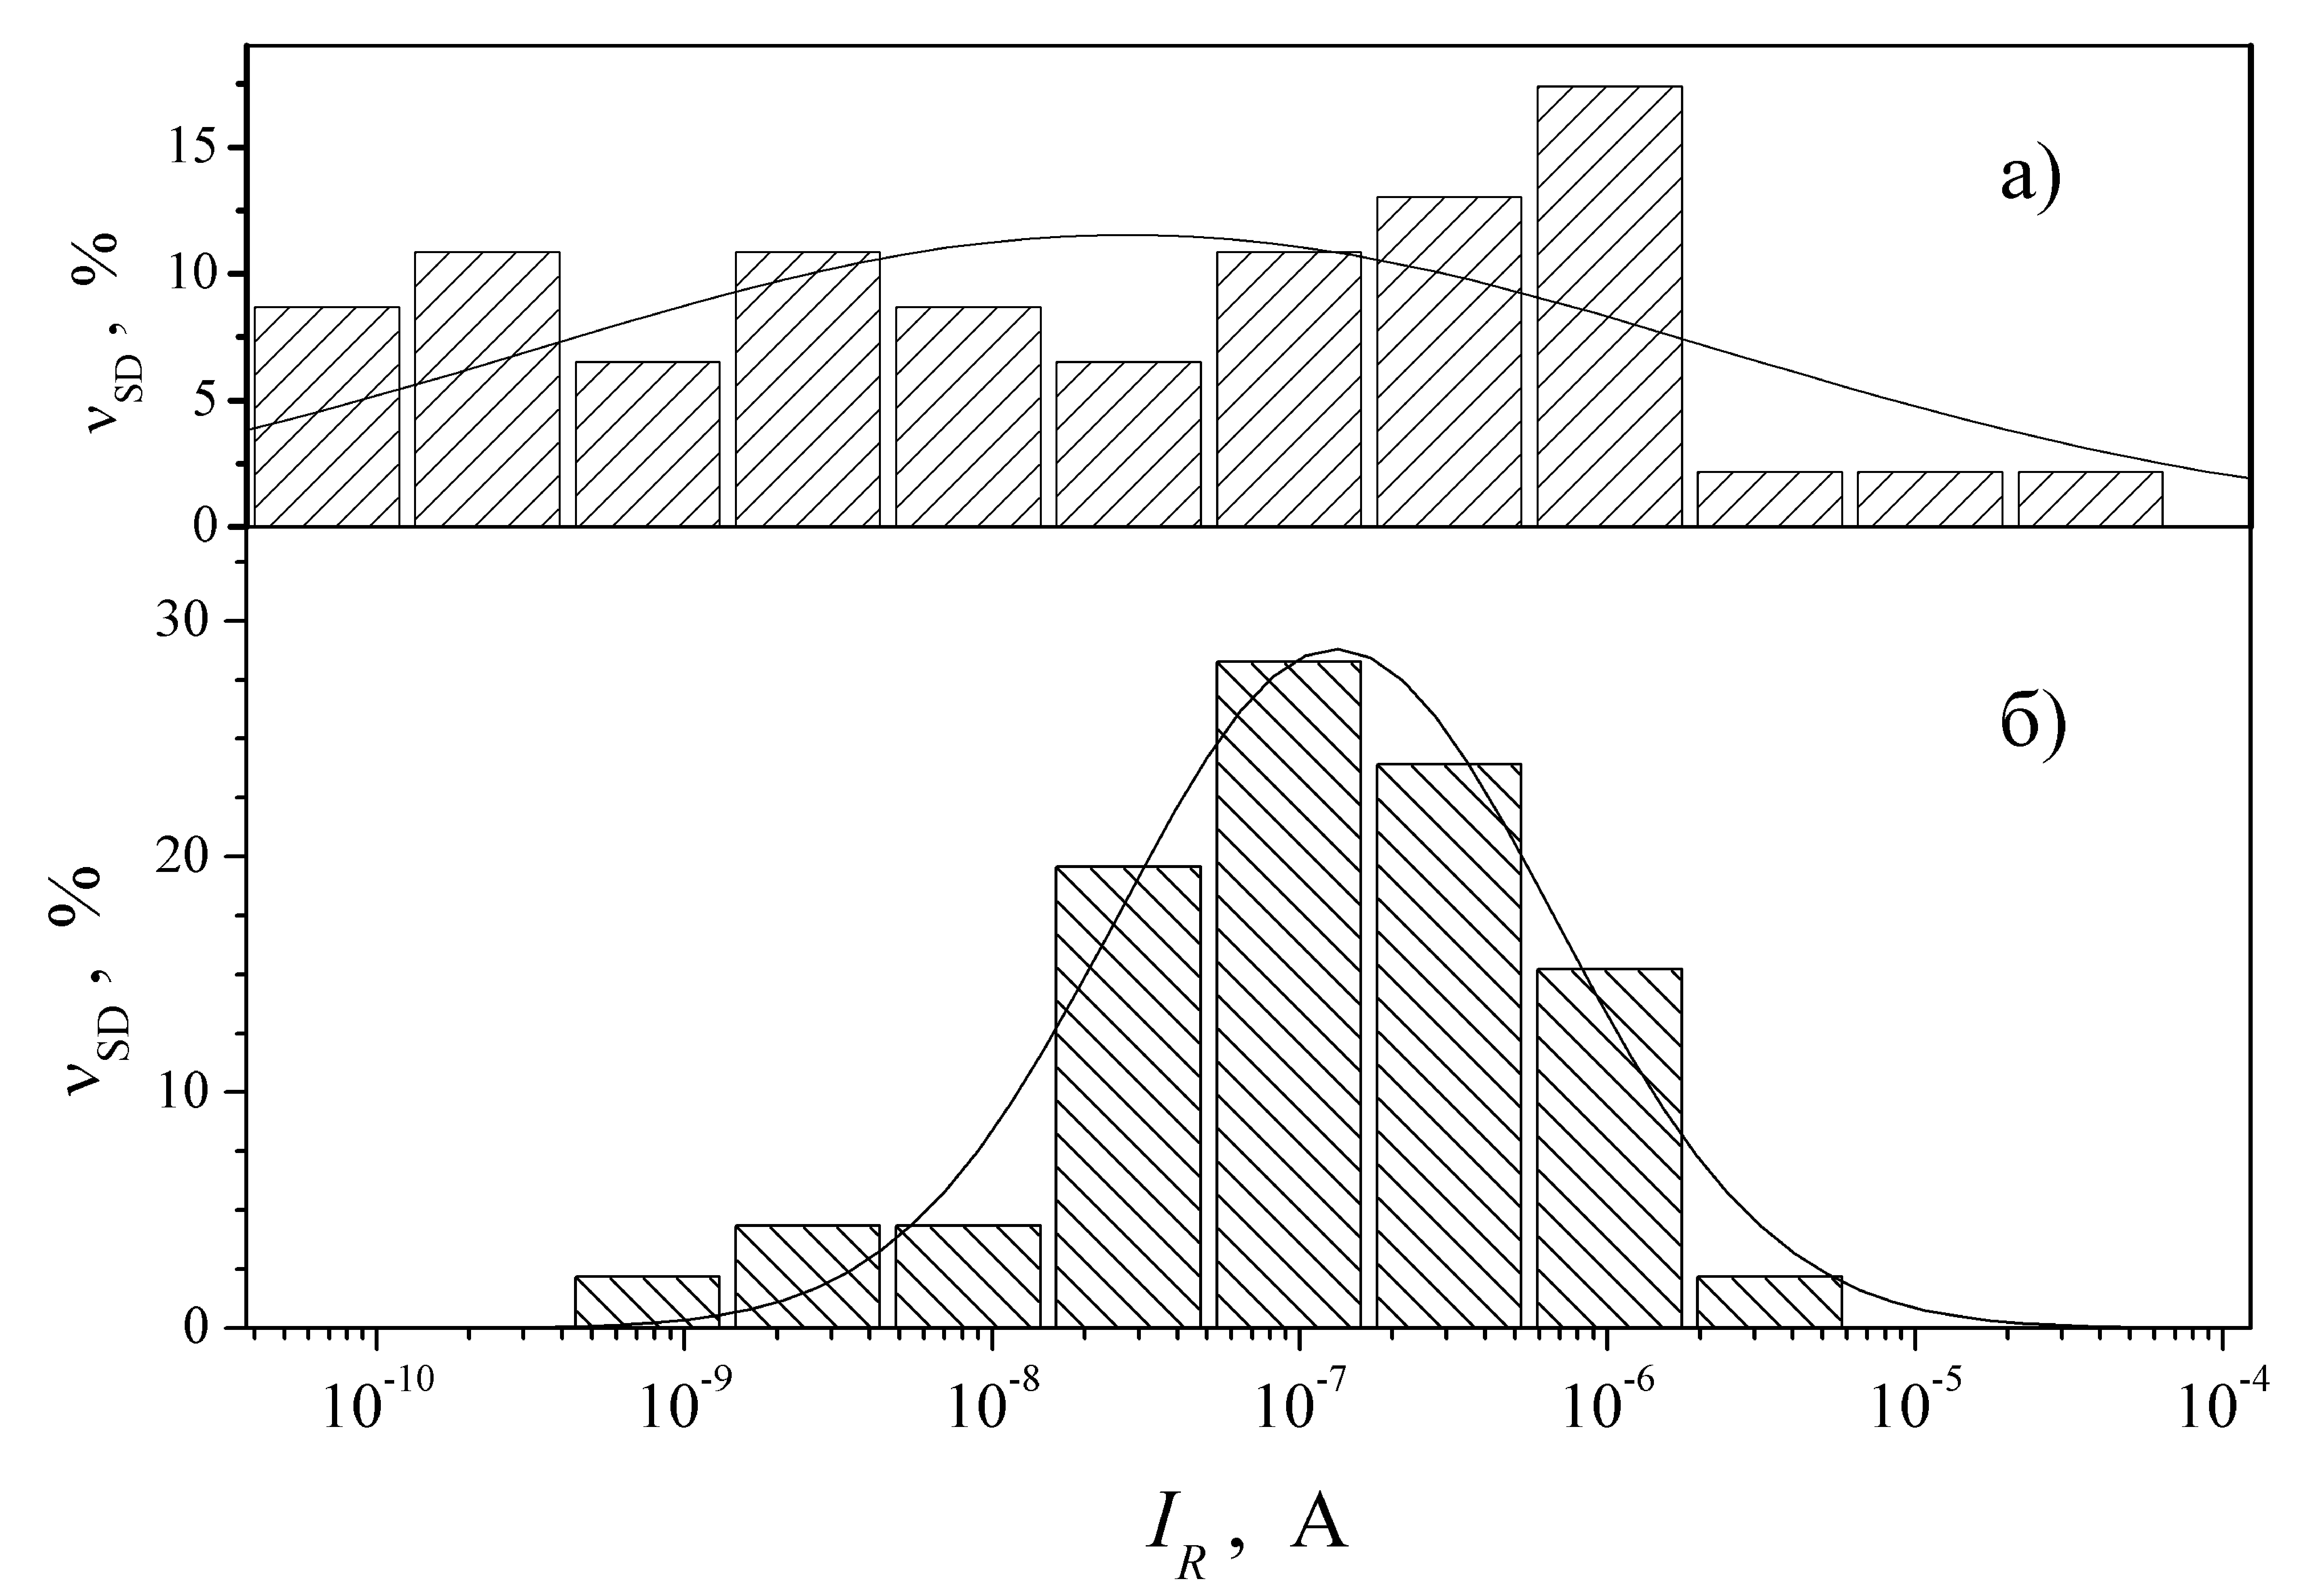
\includegraphics[width=0.7\textwidth]{figIrG_GA}%
\caption{\label{figIrG_GA}
Порівняльні розподіли величини зворотного струму (при $V_R=2$~В)
для структур Au--TiB$_x$--$n$--$n^+$--GaAs до ультразвукової обробки (а) та після неї(б).
$W_\mathtt{US}=1,8$~Вт/см$^2$, $f_\mathtt{US}=4,1$~МГц, $t_\mathtt{UST}=10$~год.
По вертикалі відкладена частка діодів, для яких струм перебуває у відповідному діапазоні.
Загальна кількість діодів --- 40.
Лінії --- апроксимація відповідно до розподілу Гауса.
Середнє значення, А:
$(2,8\pm0,2)\cdot10^{-8}$ (а),
$(1,31\pm0,01)\cdot10^{-7}$ (б).
Дисперсія:
$9\pm2$ (а),
$3,3\pm0,2$ (б)
\vspace{1em}
}
\end{figure}

\begin{figure}[t]
\center
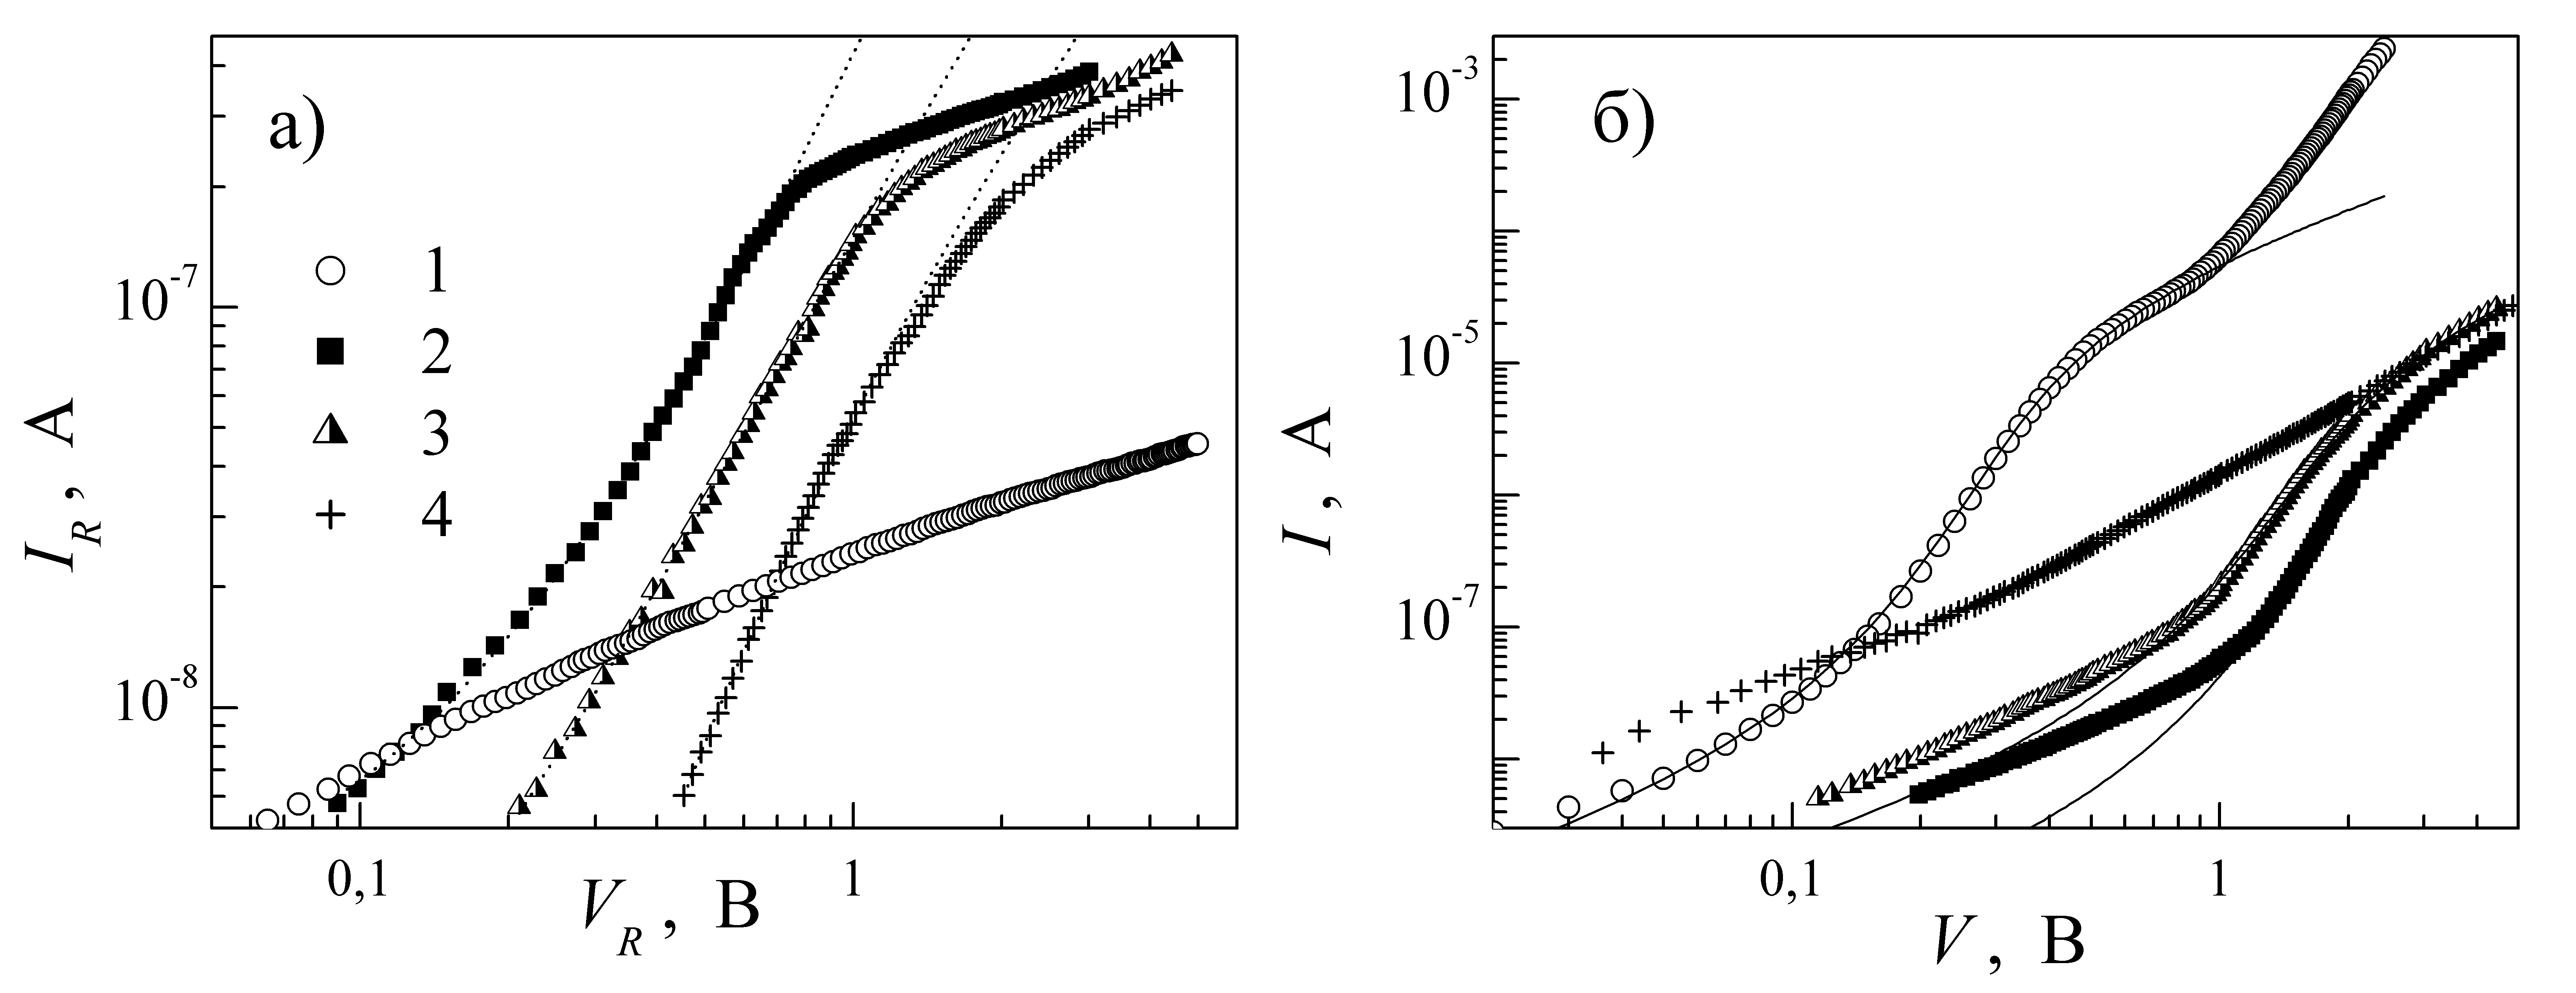
\includegraphics[width=0.85\textwidth]{figIV_MIS}%
\caption{\label{figIV_MIS}
Зворотні (а) та прямі (б) ВАХ структур Au--SiO$_2$--Si до (криві 1)
та після (2--4) опромінення $\gamma$--квантами.
$t_\mathtt{UST}$ , хв: 0 (2), 30 (3), 60 (4).
$T=300$~K.
Точки --- експеримент,
лінії --- апроксимація за формулами~(\ref{eqSDIV}) (суцільні) та (\ref{eqIVTAT}) (пунктир)
\vspace{1em}
}%
\end{figure}

У шостому розділі також повідомляється про результати досліджень, спрямованих на з'ясування можливості відновлення характеристик структур Au--SiO$_2$--Si,
деградованих внаслідок $\gamma$--опромінення ($D=5\cdot10^7$~рад).
Виявлено, що опромінення суттєво змінює процеси перенесення заряду --- рис.~\ref{figIV_MIS}.
Показано, що при малих прямих зміщеннях переважаючим стає струм, обмежений просторовим зарядом, для якого
\begin{equation}\label{eqVIsclc}
  I=I_0\,V^{\,m_\mathrm{F}},
\end{equation}
причому $I_0$ залежить від концентрації пасток $N_t$ ($I_0\sim 1/N_t^{m_\mathrm{F}-1}$),
а $m_\mathrm{F}$ відображає енергетичний розподіл їх рівнів
%\cite{Jafar}
[10$^*$].
Поява даної компоненти струму пов'язана з утворенням ненасичених зв'язків на границі Si--SiO$_2$ ($P_b$--центрів).
Накопичення $P_b$--центрами від'ємного заряду на інтерфейсі викликає зменшення ТЕ складової струму.
Опромінення також є причиною появи $E'$--центрів (вакансій кисню), що
викликає появу при зворотному зміщенні струму втрат, пов'язаного з тунелюванням по пасткам, для якого
\begin{equation}\label{eqIVTAT}
  I=I_{0,\mathrm{TAT}}\,(U_d+V_R)\exp\left(-R_\mathrm{TAT}/F_m\right),
\end{equation}
де параметр $I_{0,\mathrm{TAT}}$ пропорційний концентрації пасток.
Виявлено, що
ультразвукова обробка
($f_\mathtt{US}=4$~МГц, $W_\mathtt{US}=2$~Вт/м$^2$, $t_\mathtt{UST}=(0,5\div1)$~год) викликає зменшення концентрації
$E'$--центрів ($I_{0,\mathrm{TAT}}$ зменшується в $\sim25$~разів) та  $P_b$--центрів ($I_0$ зростає в $\sim30$~разів),
а також звуження енергетичного спектра останніх ($m_\mathrm{F}$ змінюється з 1,3 до 1,8).
Акустоіндуковані ефекти пов'язані з акустостимульованою дифузію  атомів кисню та водню, причому ефективність пасивації останніми ненасичених зв'язків залежить
від рівня механічних напруг в околі дефекту.



%\newpage
%При использовании пакета \verb!biblatex! список публикаций автора по теме
%диссертации формируется в разделе <<\publications>>\ файла
%\verb!../common/characteristic.tex!  при помощи команды \verb!\nocite!
%
%\ifdefmacro{\microtypesetup}{\microtypesetup{protrusion=false}}{} % не рекомендуется применять пакет микротипографики к автоматически генерируемому списку литературы
%\ifnumequal{\value{bibliosel}}{0}{% Встроенная реализация с загрузкой файла через движок bibtex8
%  \renewcommand{\bibname}{\large \authorbibtitle}
%  \nocite{*}
%  \insertbiblioauthor           % Подключаем Bib-базы
%  %\insertbiblioother   % !!! bibtex не умеет работать с несколькими библиографиями !!!
%}{% Реализация пакетом biblatex через движок biber
%  \ifnumgreater{\value{usefootcite}}{0}{
%%  \nocite{*} % Невидимая цитата всех работ, позволит вывести все работы автора
%  \insertbiblioauthorcited      % Вывод процитированных в автореферате работ автора
%  }{
%  \insertbiblioauthor           % Вывод всех работ автора
%%  \insertbiblioauthorgrouped    % Вывод всех работ автора, сгруппированных по источникам
%%  \insertbiblioauthorimportant  % Вывод наиболее значимых работ автора (определяется в файле characteristic во второй section)
%  \insertbiblioother            % Вывод списка литературы, на которую ссылались в тексте автореферата
%  }
%}
%\ifdefmacro{\microtypesetup}{\microtypesetup{protrusion=true}}{}

